\chapter{Applications on Sirius Storage Ring}

This final chapter is dedicated to the application to Sirius storage ring of the theory and the code presented and discussed in the previous chapters. 

During the Sirius commissioning in 2020, the implemented LOCO code had already been proven to be useful to correct Sirius linear optics and coupling, improving the machine performance. The optics and coupling corrections obtained with LOCO method also contributed for smooth operation recoveries after five~\glspl{id} installations. Only the~\gls{id} installed in a high-beta section required localized gradients compensation of $\SI{0.5}{\%}$ for the defocusing quadrupoles (QDA). The~\glspl{id} installed in low-beta sections did not perturb the storage ring in a level that could be measured. 

A few tests were performed with measured~\glspl{orm} using the electron beam in the storage ring and they are reported in Section~\ref{sec:tests_measured}. The stored current used during the measurements was around $\SI{10}{\milli\ampere}$, which is a value that provides a good accuracy for~\gls{bpm} readings and the beam stability is guaranteed as well.

The studies reported in this chapter were performed in a philosophy of scientific case. The main objective is, starting from a storage ring without any optics and coupling corrections, iteratively perform LOCO procedure and apply the calculated corrections until convergence is reached. The results from this process are presented and discussed in Section~\ref{sec:orm_fit}. From this point, independent optics and coupling measurements were performed to characterize the storage ring before and after the corrections to determine how much the study improved Sirius parameters and performance towards the expected values. Section~\ref{sec:independent_meas} is dedicated to this part.

The~\gls{orm} measurement procedure was controlled by~\gls{sofb}, the same software that drives the orbit correction. Both horizontal and vertical kicks variations used for the measurements were $\Delta \theta_x=\Delta \theta_y=\SI{15}{\micro\radian}$ and the variation in~\gls{rf} frequency was $\Delta f_{\mathrm{rf}} = \SI{80}{\hertz}$. These variations are intermediate in the sense that they provide a compromise between sufficient orbit distortion for accurate~\gls{bpm} measurements and also keep variations small enough to avoid non-linear effects. Nominally, the peak orbit distortions at~\glspl{bpm} for these corrector variations are $\Delta x = \SI{196}{\micro\meter}$ and $\Delta y = \SI{134}{\micro\meter}$. The peak horizontal distortion for the variation in~\gls{rf} frequency is $\Delta x = \SI{38}{\micro\meter}$. The~\gls{orm} typical measurement time for Sirius storage ring is $25$ minutes.

Sirius storage ring status when these studies were performed was: four undulators were installed, one in a high-beta section and three in low-beta sections; the~\gls{bba} procedured was applied to obtain~\glspl{bpm} offsets relative to quadrupoles centers and these offsets were used as the target orbit for orbit correction. The~\gls{std} of residual orbit obtained in both planes was around $\SI{30}{\micro\meter}$. During commissioning, operating the machine with nominal betatron tunes ($\nu_x = 49.096$ and $\nu_y = 14.152$) produced a very low injection efficiency (less than $10\%$). After scanning the tunes, the values that provided a better injection efficiency were $\nu_x = 49.075$ and $\nu_y = 14.134$. Therefore, tunes close to these values were used throughout the commissioning and this study as well. Nevertheless, without optics and coupling correction the injection efficiency was only $20\%$ on average, with large pulse-by-pulse variations.
\section{Tests with Measured Data}\label{sec:tests_measured}
A few tests were performed with data measured in the actual storage ring to check the method reliability in practice as well. Moreover, some tests allowed to confirm the code setup, related to the minimization method and constraints on quadrupoles variations. The tests also provided information about random errors of fit parameters.

The beam orbit was measured with~\glspl{bpm} during $\SI{10}{\second}$ with a measurement rate of $\SI{25}{\hertz}$. The average variation obtained for each plane was $\sigma_{\mathrm{BPM}, x} = \SI{0.162(6)}{\micro\meter}$ and $\sigma_{\mathrm{BPM}, y} = \SI{0.233(7)}{\micro\meter}$. These values represent the noise level of positions measurements provided by~\glspl{bpm} in Sirius storage ring. This means that even if the machine matched the model perfectly, this level of discrepancy in the~\gls{orm} residue is expected.

\subsection{Relevance of Constraints}\label{subsec:loco_config}
From tests with simulated model and jacobian matrix analysis discussed in Subsection~\ref{subsec:jacobian_analysis}, the chosen LOCO configuration was: 1) include the parameters presented in Table~\ref{tab:fit_params} in the fitting, 2) use~\gls{lm} method as the minimization algorithm setting initially $\lambda = 10^{-3}$, 3) use the $\Delta K$ constraints with weight $c_{\Delta K} = 10^{3}$, 4) remove only the last singular value for pseudo-inversion of LOCO jacobian matrix. 

In order to check if this setup is appropriated for LOCO analysis in the actual Sirius storage ring a simple test was performed. Without any optics or coupling corrections applied in the storage ring, an~\gls{orm} was measured and it was used to apply LOCO fitting with two setups: without any modification (using~\gls{gn} method and no constraint on $\Delta K$) and with the chosen configuration. The initial $\chi$ for the measured~\gls{orm} was $\SI{24.6}{\micro\meter}$ and for both LOCO fittings, $\chi$ converged to values close to $\SI{0.9}{\micro\meter}$. However there is a great difference between the two calibrated models regarding the quadrupole deviations from the nominal values. As discussed in Chapter~\ref{chap:loco}, without constraints on $\Delta K$, the LOCO process tries to minimize $\chi$ without any concern on the quadrupoles deviations magnitudes, which may lead to large excursions in these parameters due to the quasi-degeneracies in LOCO jacobian. With constraints on $\Delta K$, the convergence path for $\chi$ is changed in order to minimize the step size of quadrupole deviations. This difference in the fitting behavior can be revealed with a plot of $\chi$ versus the~\gls{std} of quadrupole changes over iterations, as presented in Figure~\ref{fig:chi_vs_dkl}. The comparison of final fit variations for the 270 quadrupoles in Sirius storage ring in this test is plotted in Figure~\ref{fig:dkl_compare}. 
\begin{figure}
\centering
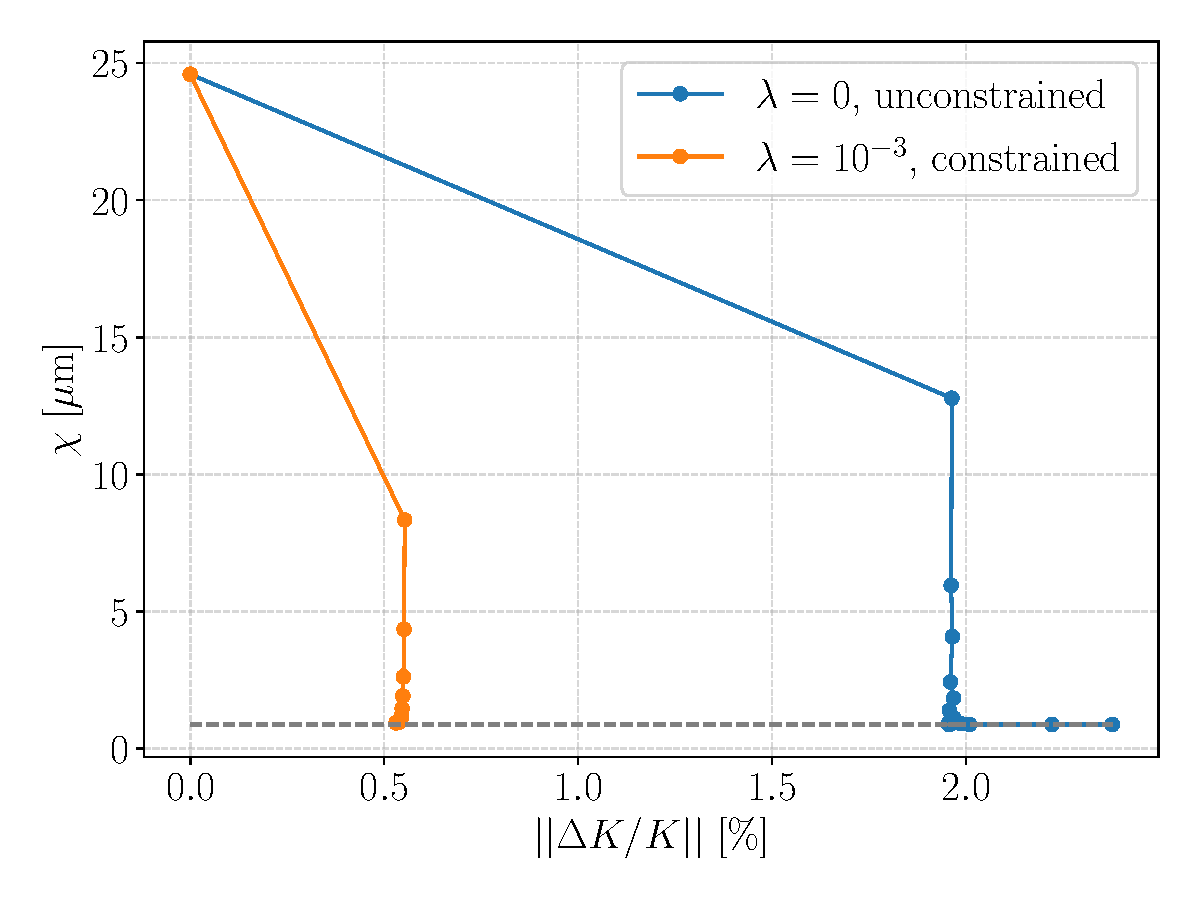
\includegraphics[width=0.75\textwidth]{figures/chi_versus_dk_cumsum.pdf}
\caption{$\chi$ versus $||\Delta K/K||$ throughout 10 LOCO iterations. The gray dashed horizontal line corresponds to $\chi = \SI{0.91}{\micro\meter}$, the value used as reference for convergence.}
\label{fig:chi_vs_dkl}
\end{figure}
\begin{figure}
\centering
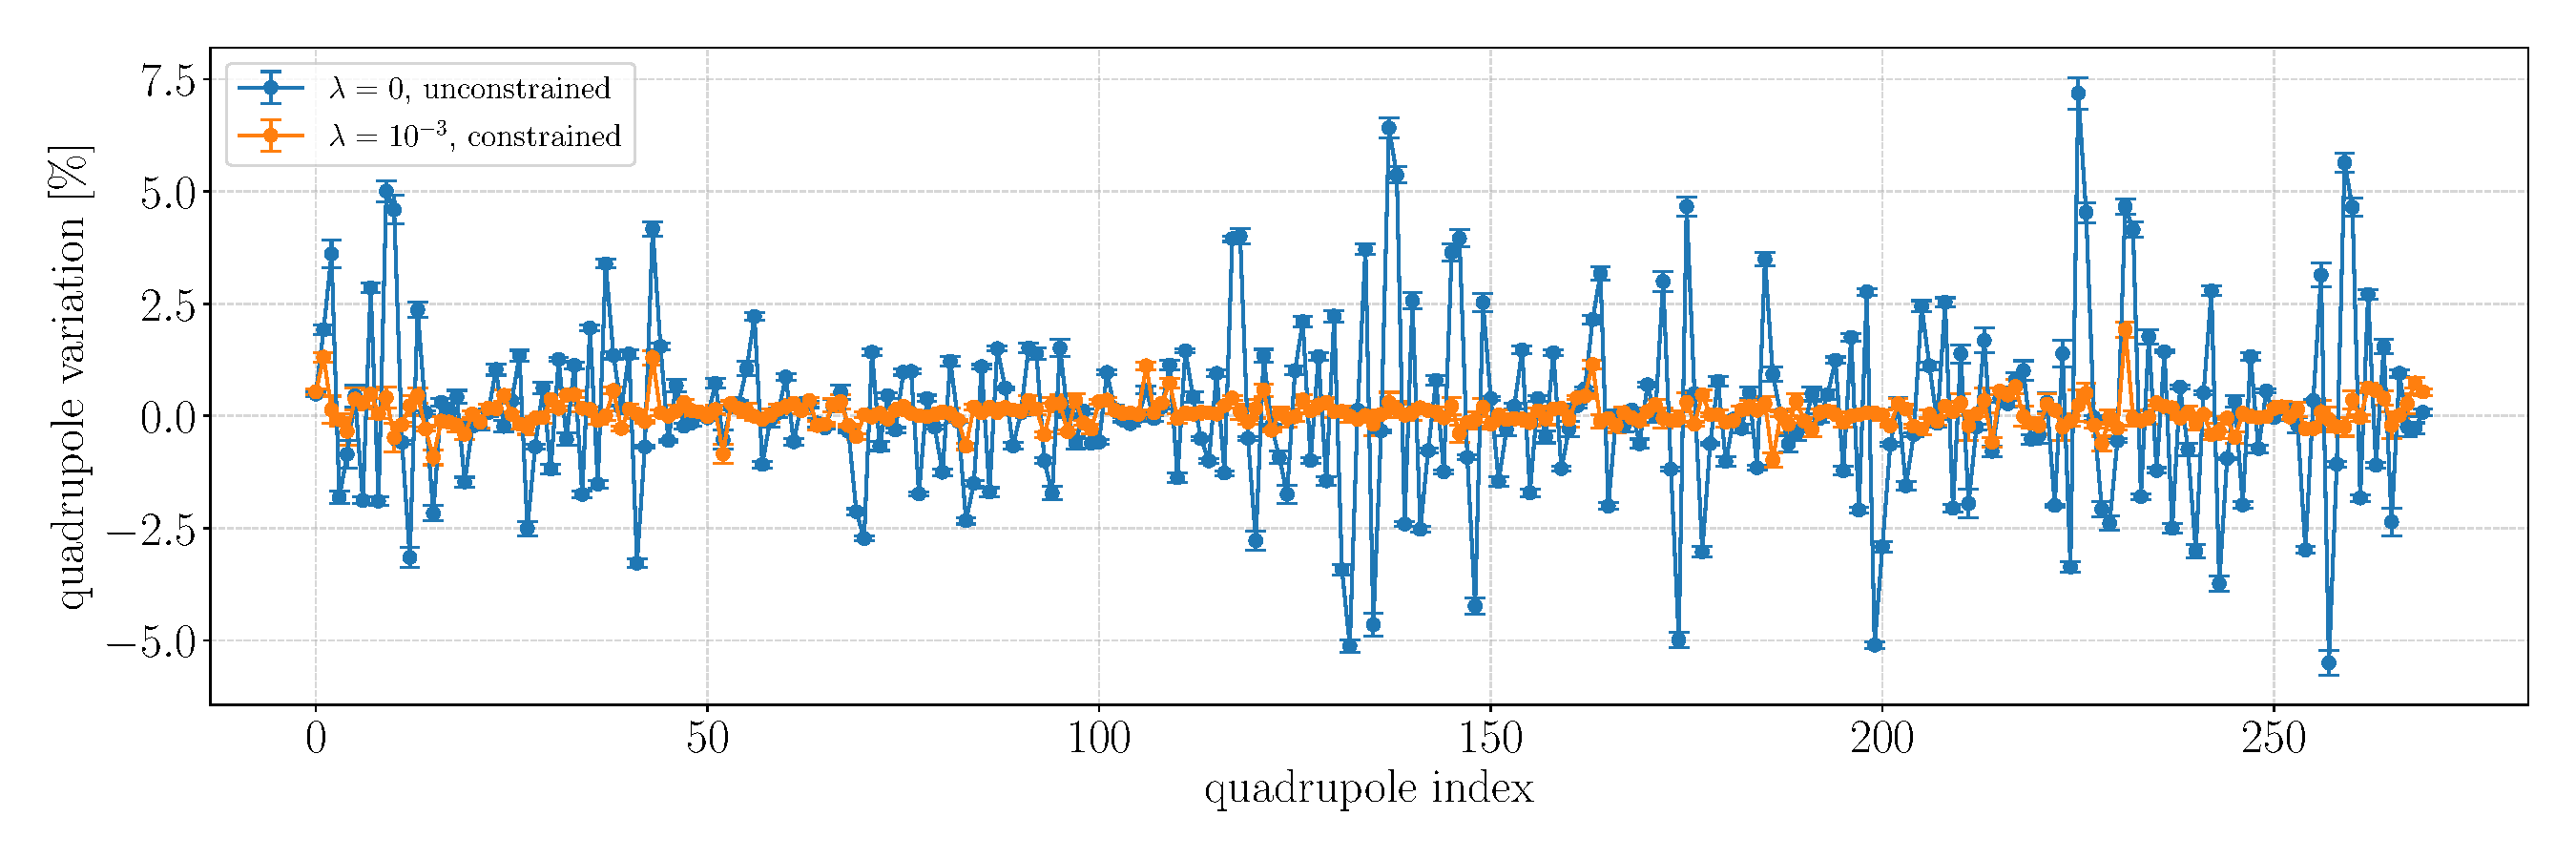
\includegraphics[width=1.0\textwidth]{figures/delta_kl_comparison_better_grid.pdf}
\caption{Comparison of quadrupoles variations obtained from LOCO with two calculation methods.}
\label{fig:dkl_compare}
\end{figure}

Previous magnetic measurements and characterizations indicate a good gradient field quality for quadrupoles, satisfying the specification of $\SI{0.05}{\%}$ in gradient errors. Moreover, it can be seen that some adjacent quadrupoles have large variations with opposite signs, which are related to the quasi-denegeracies discussed in Section~\ref{sec:degeneracy}. Nevertheless, the large quadrupoles variations represented in Figure~\ref{fig:dkl_compare} were applied in the storage ring and, after that, it was observed that the errors of measured optics parameters were actually increased. This is a strong evidence that the large variations reaching $\SI{7.5}{\%}$ are unrealistic. The solution obtained with constraints demands much less of quadrupole variations and also adjusts the measured~\gls{orm} in the same level. Applying the quadrupole variations obtained with constraints resulted in positive effects on the storage ring optics. The variations obtained for the other fit parameters included in the fitting agree for the two setups within the error bars, which was expected since basically the major difference is related to the constraints on quadrupoles strengths.

It is important to point out that the convergence criteria for $\chi$ should avoid the cases of over-fitting. In addition to spare LOCO running time, the most important reason is to prevent the method from increasing the quadrupoles strengths to produce a negligible reduction in $\chi$. In Figure~\ref{fig:chi_vs_dkl} it can be seen that for the unconstrained case, the last three iterations increased $||\Delta K/K||$ considerably while $\chi$ was basically the same. The over-fitting is more serious for the unconstrained case indeed, since each iteration may produce large variations on quadrupoles but it may also be a problem even for the constrained case, since accumulated small step sizes may also produce large and unnecessary variations in the final values. The convergence criteria can be controlled by defining a minimum acceptable change in the residue, given by $\chi_{\mathrm{step}}$, and a minimum level for the residue, given by $\chi_{\mathrm{min}}$. For LOCO fittings performed in Sirius storage ring, the values used was $\chi_{\mathrm{step}} = \SI{0.01}{\micro\meter}$ and $\chi_{\mathrm{min}} = \SI{0.25}{\micro\meter}$, where the value for $\chi_{\mathrm{min}}$ was defined based on Sirius \glspl{bpm} accuracy. The final residue of $\SI{0.91}{\micro\meter}$ obtained in these fittings is still $3.6$ times larger than the~\gls{bpm} accuracy and a possible explanation for this limit of convergence will be discussed in Section~\ref{sec:orbit_effect}. Nevertheless, a calibrated model with an~\gls{orm} that agrees with the measured in the sub-$\mu$m level typically corresponds to a good fitting~\cite{safranek1997}.

\subsection{Random Errors}\label{subsec:fit_var}
As mentioned in~\cite{safranek1997}: ``\textit{the easiest way to determine how much the set of fit parameters vary due to random errors in the measurements is simply to measure many~\gls{orm}, analyze each one separately, and see how much variation there is between fit parameters for the different data sets}''. Therefore, to access the random errors associated with the fit parameters presented in Table~\ref{tab:fit_params}, the aforementioned procedure was applied in Sirius storage ring, where 10~\glspl{orm} were measured sequentially. 

\gls{loco} analysis was performed in these 10 measured~\glspl{orm} with the configuration described in Subsection~\ref{subsec:loco_config} and the results are organized in Table~\ref{tab:fit_var} with the~\gls{rms} variations. The average initial residue for these 10 realizations was $\chi_{\mathrm{initial}} = \SI{9.2(4)}{\micro\meter}$ and after the convergence the average final residue was $\chi_{\mathrm{final}} = \SI{1.04(2)}{\micro\meter}$. For each fit parameter, the~\gls{std} variation obtained in the set of 10 LOCO realizations was used to define the corresponding error bars. For each calibrated model obtained with LOCO, the lattice functions and its variations in this set of 10 values were also calculated. The results are organized in Table~\ref{tab:twiss_var}\footnote{The initial $\chi$ and the values for normal and skew quadrupoles variations in Table~\ref{tab:twiss_var} are relatively low because this repeatability test was performed after the LOCO corrections application to the storage ring.}. 
% \begin{table}
%     \centering
%     \caption{Variations in fit parameters from LOCO analysis of 10 ORM measurements performed in Sirius storage ring.}
%     \label{tab:fit_var}
%     \begin{tabular}{cccc}
%         \toprule\toprule
%         Parameter & std variation & peak-to-valley variation & Unit \\
%         \hline
%         Quadrupole Relative Strength     & 0.13 & 0.32 & \% \\  
%         H. BPM Gain             & 0.06 & 0.27 & \%\\
%         H. Corrector Gain       & 0.18 & 1.03 & \%\\
%         V. BPM  Gain             & 0.07 & 0.35 & \%\\
%         V. Corrector Gain       & 0.21 & 1.14 & \%\\
%         Skew Quadrupole Absolute Strength& \num{1.3e-4} & \num{6.2e-4} & $\SI{}{\meter^{-1}}$\\
%         BPM roll angle                & 0.25 & 1.31 & $\SI{}{\milli\radian}$ \\
%         \bottomrule\bottomrule
%     \end{tabular}
% \end{table}
% \begin{table}
%     \centering
%     \caption{Variations in lattice functions obtained from LOCO calibrated models from 10 ORM measurements performed in Sirius storage ring.}
%     \label{tab:twiss_var}
%     \begin{tabular}{cccc}
%         \toprule\toprule
%         Lattice function & std variation & peak-to-valley variation & Unit \\
%         \hline
%         $\beta_x$ & \num{0.17}& \num{0.86} & \%\\
%         $\beta_y$ & \num{0.14} & \num{0.99}& \% \\
%         $\eta_x$ & \num{0.26} & \num{1.36} & \SI{}{\milli\meter}\\
%         $\eta_y$ & \num{0.62} & \num{2.62} & \SI{}{\milli\meter} \\
%         \bottomrule\bottomrule
%     \end{tabular}
% \end{table}
\begin{table}
    \centering
    \caption{Variations in fit parameters from LOCO analysis of 10 ORM measurements performed in Sirius storage ring.}
    \label{tab:fit_var}
    \begin{tabular}{cccc}
        \toprule\toprule
        Parameter & mean rms & rms variation & Unit \\
        \hline
        Quadrupole Relative Strength      & 0.17 & 0.13 & \% \\ 
        H. BPM Gain                      & 96.5 & 0.2 & \%\\
        H. Corrector Gain                & 92.4 & 0.6 & \%\\
        V. BPM  Gain                     & 96 & 4 & \%\\
        V. Corrector Gain                & 94 & 4 & \%\\
        Skew Quadrupole Strength& \num{7.5e-4} & \num{3.4e-4} & $\SI{}{\meter^{-1}}$\\
        BPM roll angle                   & 3.1 & 0.8 & $\SI{}{\milli\radian}$ \\
        \bottomrule\bottomrule
    \end{tabular}
\end{table}
\begin{table}
    \centering
    \caption{Variations in lattice functions obtained from LOCO calibrated models from 10 ORM measurements performed in Sirius storage ring.}
    \label{tab:twiss_var}
    \begin{tabular}{cccc}
        \toprule\toprule
        Lattice function error & mean rms & rms variation & Unit \\
        \hline
        $\Delta\beta_x/\beta_x$ & \num{0.8}& \num{0.5} & \%\\
        $\Delta\beta_y/\beta_y$ & \num{0.5} & \num{0.4}& \% \\
        $\Delta\eta_x$ & \num{2.5} & \num{0.5} & \SI{}{\milli\meter}\\
        $\Delta\eta_y$ & \num{12.6} & \num{1.6} & \SI{}{\milli\meter} \\
        \bottomrule\bottomrule
    \end{tabular}
\end{table}

The variations for dispersion function are calculated as absolute values because $\eta_x$ is zero in the straight sections, so the division to obtain a finite relative variation is not possible. In the case of betatron functions, which always assume positive values by definition, it is possible to obtain the relative variations.
% Just for comparison of the magnitude of the variations presented in Table~\ref{tab:twiss_var}, the average and~\gls{std} of $\eta_x$ around the Sirius storage ring is $\SI{2.1}{\cm}$ and the peak-to-valley value is $\SI{8.3}{\cm}$. 
\subsection{Initial Condition Dependence}
The~\gls{orm} fitting for Sirius storage ring with LOCO can be viewed as finding a minimum of a function $\chi\left(\Vec{P}\right)$ with $1110$ variables, the fit parameters. A strategy to explore the topology of local minima in the solution space is beginning the fitting with different initial conditions and then check the final solution obtained. If the final results are fairly independent on the initial guess, one has an indicative that, at least inside the region covered by the initial guesses range, the obtained solution is the best minimum. For a given problem, if the initial guesses cover a broad range of feasible values for fit parameters, this process indicates that, amongst the doable solutions, the found solution is the best one.

The initial condition dependence test was applied in LOCO code. An~\gls{orm} measured in Sirius storage ring was used as input for LOCO fitting. Twenty different initial conditions, regarding only the quadrupole strengths, were used to adjust the measured~\gls{orm}. The initial guesses varied with a random normal distribution with $\sigma=0.5\%$ and one $\sigma$ cutoff, with respect to the nominal gradients. Larger values of $\sigma$ were tested but they produced unstable dynamics in the model or, for the stable cases, the algorithm did not converge. Thus $0.5\%$ was chosen since it allowed for the largest feasible initial conditions.

All the 20 initial conditions produced a greater initial $\chi$ as compared to the nominal initial guess. The minimum initial $\chi$ was $\SI{25.2}{\micro\meter}$ while with zero initial condition it was $\SI{24.6}{\micro\meter}$. The $\chi$ convergence for all the 20 realizations and the zero initial guess are plotted in Figure~\ref{fig:chi_ini_guess}. The initial $\chi$ in this test was $\SI{47(28)}{\micro\meter}$ and after 10 iterations, the final was $\SI{0.98(7)}{\micro\meter}$. Therefore, all the realizations converged to the same fitting level.
\begin{figure}
\centering
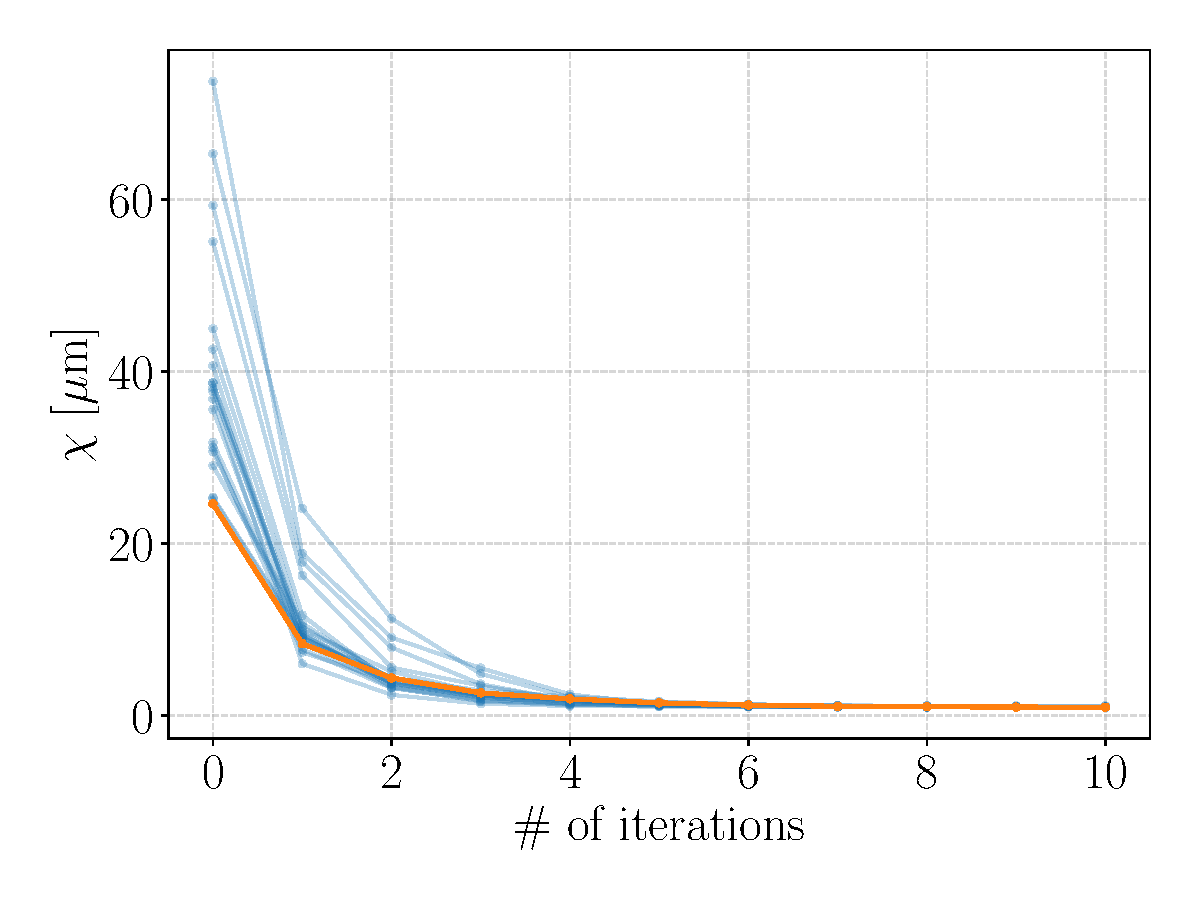
\includegraphics[width=0.75\textwidth]{figures/chi_convergence_initial_guess.pdf}
\caption{$\chi$ convergence for different initial conditions. The zero initial guess convergence is represented by the orange curve.}
\label{fig:chi_ini_guess}
\end{figure}

Figure~\ref{fig:quad_stren_ini_guess} shows the gradient solutions obtained with these 20 different initial conditions and the solution obtained with zero initial guess as well. The relative variations were calculated comparing the final results with the nominal strengths. Although the initial spread in gradients was $0.5\%$, the final spread in the fitted solutions is $0.2\%$. The spread in the obtained solution by varying the initial conditions are within the fit parameters error bars. Moreover, the correlation between the mean of solutions and the solution obtained with zero initial guess was $98.5\%$ and the~\gls{std} difference is only $0.06\%$. For the realizations individually, the maximum and minimum correlations was $90\%$ and $71\%$, respectively. With this test, one can conclude that the solution obtained with the nominal model as the starting point (zero initial guess) is fairly independent of initial conditions. Therefore, given the explored range in the solutions space with random initial conditions, this solution is the unique local minimum.
\begin{figure}
\centering
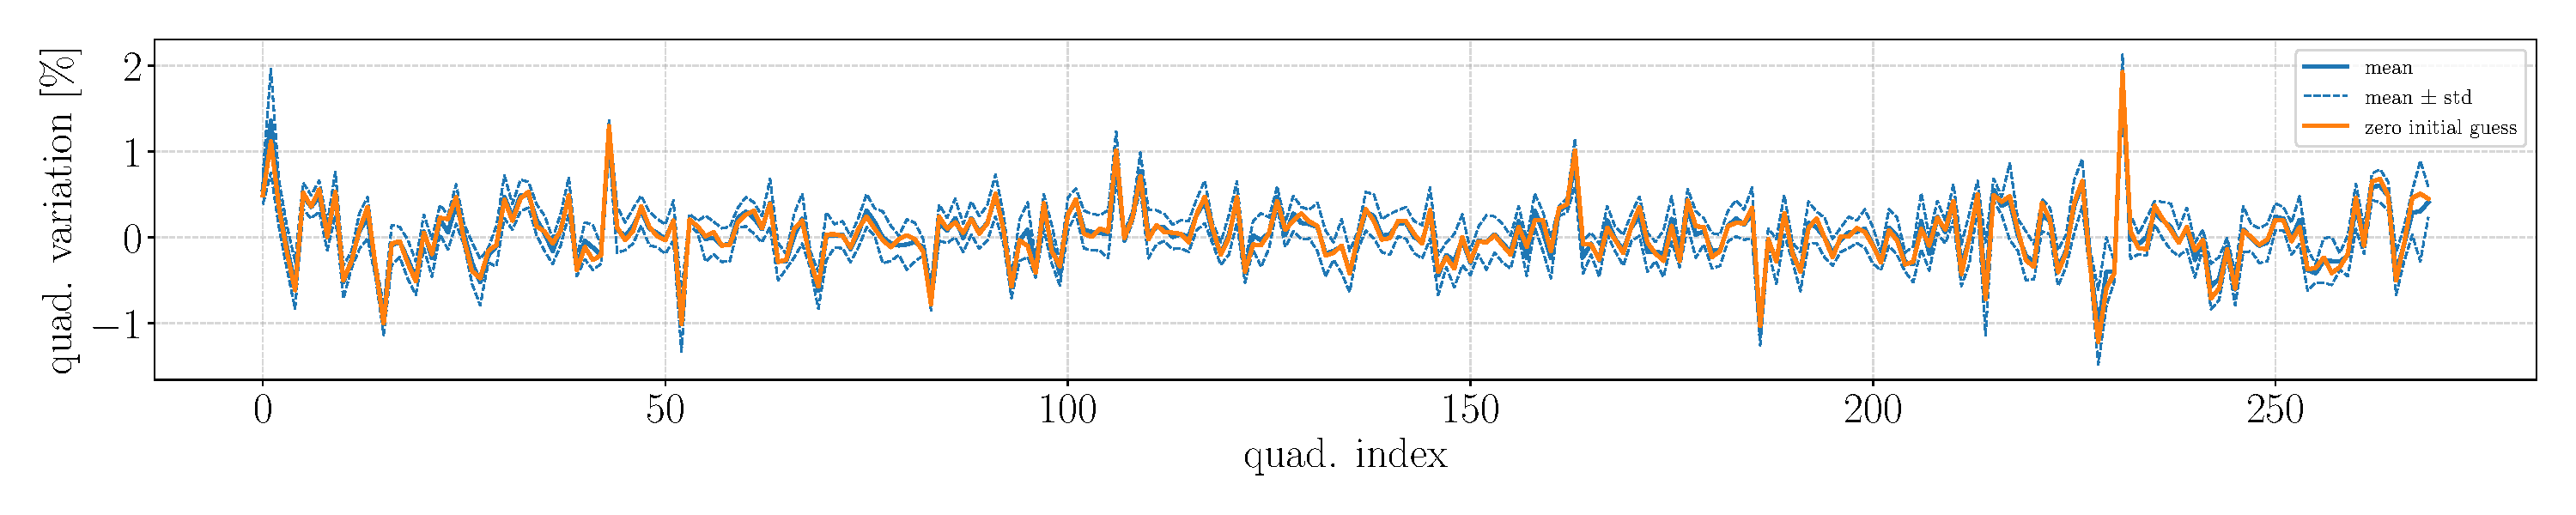
\includegraphics[width=1.0\textwidth]{figures/quad_stren_initial_guess.pdf}
\caption{Quadrupoles variations for 20 different initial guesses compared to zero initial condition.}
\label{fig:quad_stren_ini_guess}
\end{figure}
\subsection{Finding Planted Error}
There is another insightful test, suggested and performed in~\cite{safranek1997}, with the goal of showing that quadrupole gradients can be accurately predicted with LOCO method. The test is quite simple: measure an~\gls{orm}, then change an individual quadrupole strength (in the case of Sirius, change the current of a trim-coil) and re-measure the~\gls{orm}. Each~\gls{orm} is adjusted with LOCO and the difference between the two sets of fitted quadrupole gradients should reveal the intentional change.

The test was also performed in Sirius storage ring. The trim-coil current of a QFA quadrupole was varied to produce a $-1.19\%$ change in its gradient strength. This quadrupole is placed in a high-beta straight section. Following the quadrupoles ordering around the storage ring, this corresponds to the 161\ts{th} quadrupole out of 270. Figure~\ref{fig:delta_13M1_qfa} shows the test results.
\begin{figure}
\centering
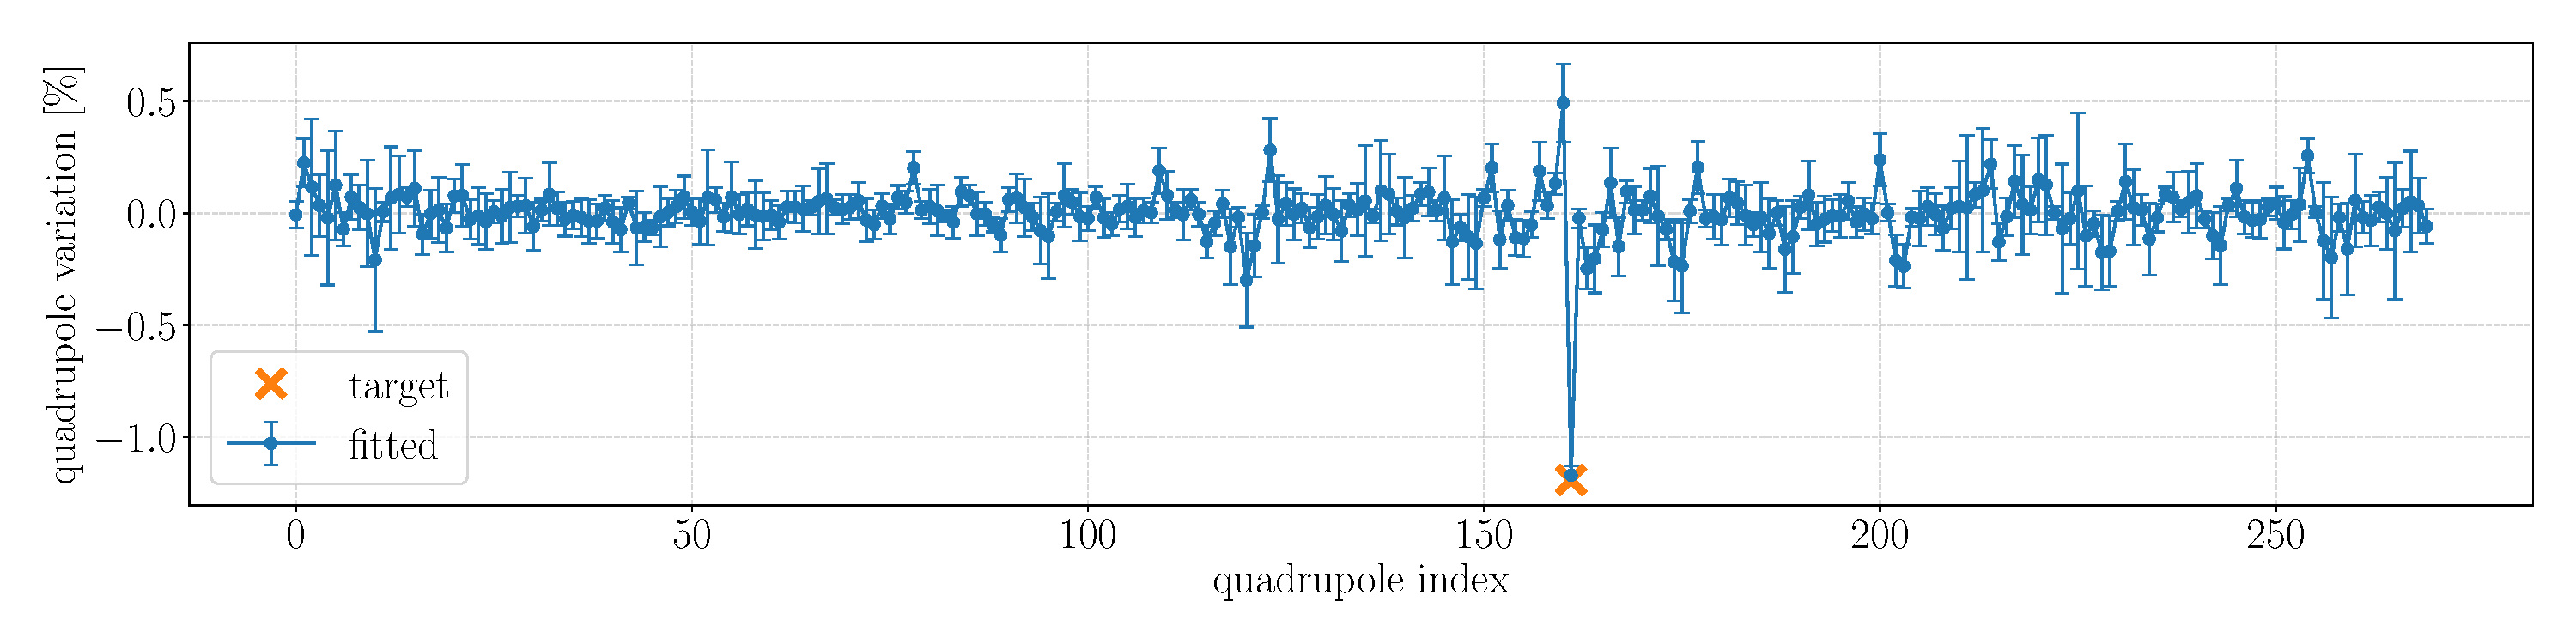
\includegraphics[width=1.0\textwidth]{figures/delta_13M1_QFA_errorbar.pdf}
\caption{Difference between quadrupole variations obtained from two ORM fittings, one ORM measured with an intentional change in the 161\ts{th} quadrupole and the other ORM measured without it.}
\label{fig:delta_13M1_qfa}
\end{figure}

The target gradient error in the 161\ts{th} quadrupole was $-1.19\%$. With LOCO, it was found a $\SI{-1.17(9)}{\%}$ variation in this quadrupole. Using the $3\sigma$ as the criteria for detecting outliers, one could also state that the $0.5\%$ variation in the 160\ts{th} quadrupole is another possible intentional change. This indicates that there is a residual degeneracy between adjacent quadrupoles that the $\Delta K$ constraints could not eliminate completely. Even so, the change in the 161\ts{th} quadrupole stands out as a $13\sigma$ variation. From this test, it can be concluded that LOCO analysis can accurately predict the quadrupole gradient errors in Sirius storage ring. 

\section{Optics Correction with LOCO}\label{sec:orm_fit}
After several tests to check the reliability of LOCO code and to define the fitting setup, the method was finally used to fit the measured~\gls{orm}, calculate the necessary corrections and apply them in Sirius storage ring normal quadrupole trim-coils and skew quadrupoles. The process was repeated until measured and nominal~\gls{orm} coincide in a satisfactory level.

The first~\gls{orm} was measured in Sirius storage ring with a $\SI{10}{\milli\ampere}$ stored electron beam and the orbit corrected to the~\gls{bba} orbit. The operation tunes were around $\nu_x = 49.07$ and $\nu_y = 14.13$, the quadrupole trim coils and skew quadrupoles currents were all set to zero. LOCO fitting was performed, starting from the nominal model to obtain the fit parameters presented in Table~\ref{tab:fit_params} that best explain the measured~\gls{orm}. Since the aforementioned tunes provide a better injection efficiency, it was decided that LOCO corrections should not move the measured tunes towards the nominal values. Therefore, the nominal model used as the initial model for LOCO had its betatron tunes shifted to match the measured values. In this way, the gradient variations should keep the tunes unchanged.

Based on previous tests performed with measured data, it was observed that only including the orbit response related to~\gls{rf} frequency variation in the~\gls{orm}, i.e., including the dispersion function in the fitting, was not sufficient to produce the correspondence between predicted and measured dispersion functions, both horizontal and vertical. The conversion factor of Eq.~\eqref{eq:chi2_disp} used was $c_{f_{\mathrm{rf}}, \theta} = \Delta f_{\mathrm{rf}}/\Delta \theta = \SI{80}{\hertz}/\SI{15}{\micro\radian}$. It was necessary to include a weight factor of $2$ in the dispersion term to obtain a better fitting of the measured dispersion. In principle, if optics distortions are caused solely by gradient errors on quadrupoles, once the measured~\gls{orm} is adjusted with the model, i.e., the beta function and phase advances in~\glspl{bpm} and correctors are fitted, the predicted dispersion function from this model should be very close to the measured dispersion. The need for this weight on dispersion is important and will be further discussed in Section~\ref{sec:orbit_effect}.

The initial difference between measured and nominal~\gls{orm} produced $\chi = \SI{24.6}{\micro\meter}$. After LOCO fitting, the calibrated model produced an~\gls{orm} whose difference to the measured one was $\chi = \SI{0.9}{\micro\meter}$. The minimum $\chi$ obtained from LOCO fitting was almost $4$ times greater than the measured BPM accuracy. Even though the obtained $\chi$ around $\SI{1}{\micro\meter}$ represents a good level of fitting, the factor $4$ difference from the BPM accuracy values indicates that there are still some systematic errors influencing the measurements, as discussed in \cite{safranek1997}.

\subsection{BPM and Corrector Gains}
\glspl{bpm} gains, roll errors and correctors gains are parameters that are related to the correspondent devices, thus it should be independent of the machine optics and coupling. Furthermore, typically these parameters should not vary significantly, especially in a short-term period. Therefore, it is reasonable to include the gains and roll errors as LOCO fit parameters in the first iteration and use these obtained values as initial conditions for the following fittings. It is expected that the gains do not deviate too much from the fit values obtained in the first step. From the first LOCO iteration on Sirius, the BPM gains, roll errors and correctors gains obtained are shown in Figure~\ref{fig:gain_fit}.
\begin{figure}
\centering
\begin{subfigure}[t]{0.49\textwidth}
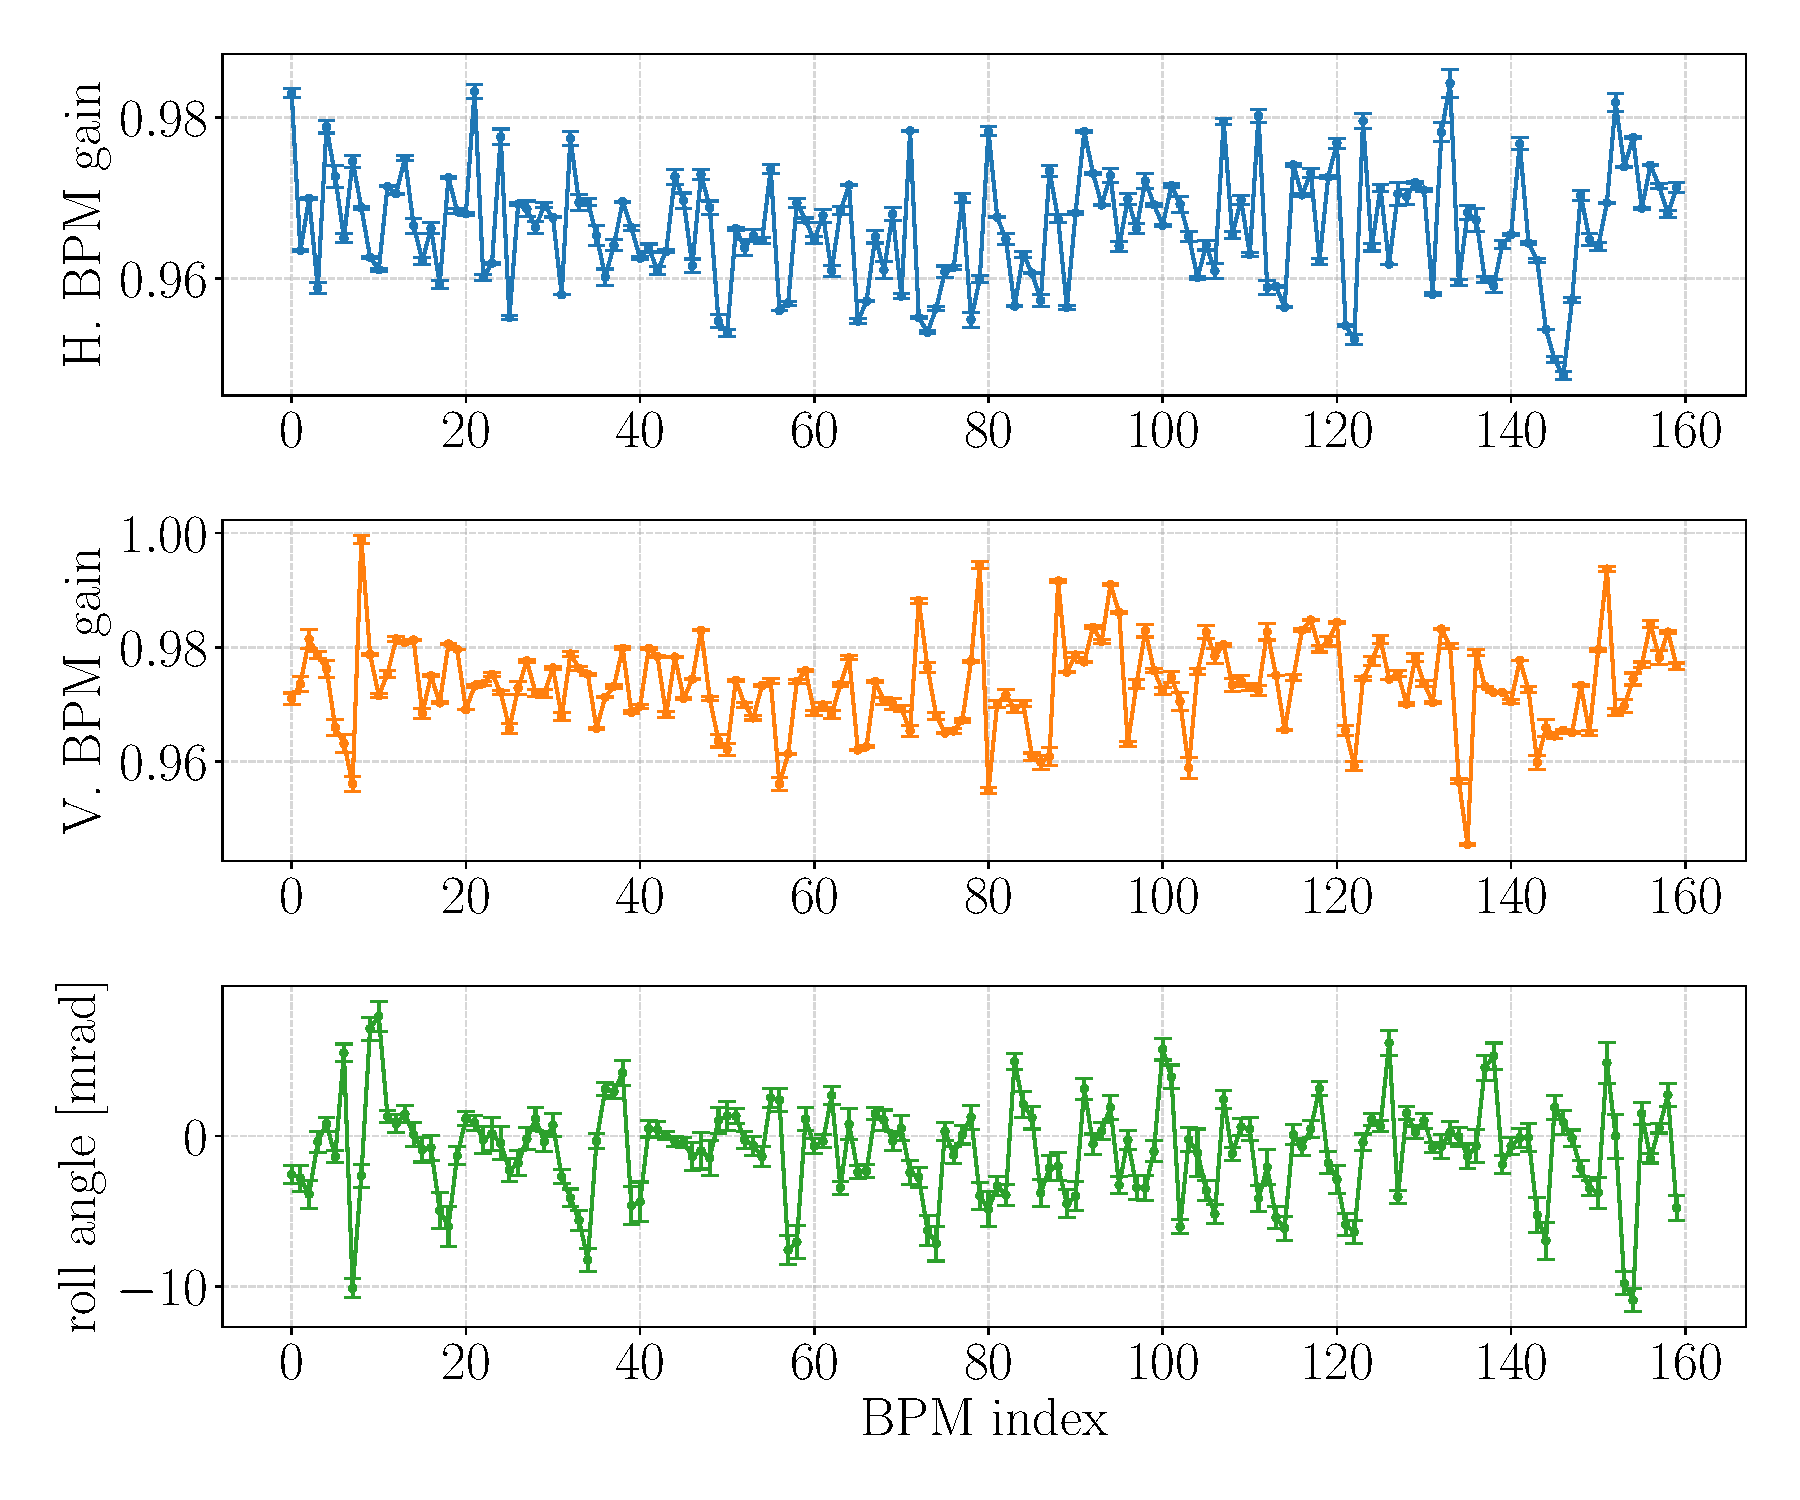
\includegraphics[width=1.0\textwidth]{figures/bpm_gains_iter0_big.pdf}
    \caption{BPM gains and roll angles.}
    \label{subfig:bpm_fit}
\end{subfigure}
 \begin{subfigure}[t]{0.49\textwidth}
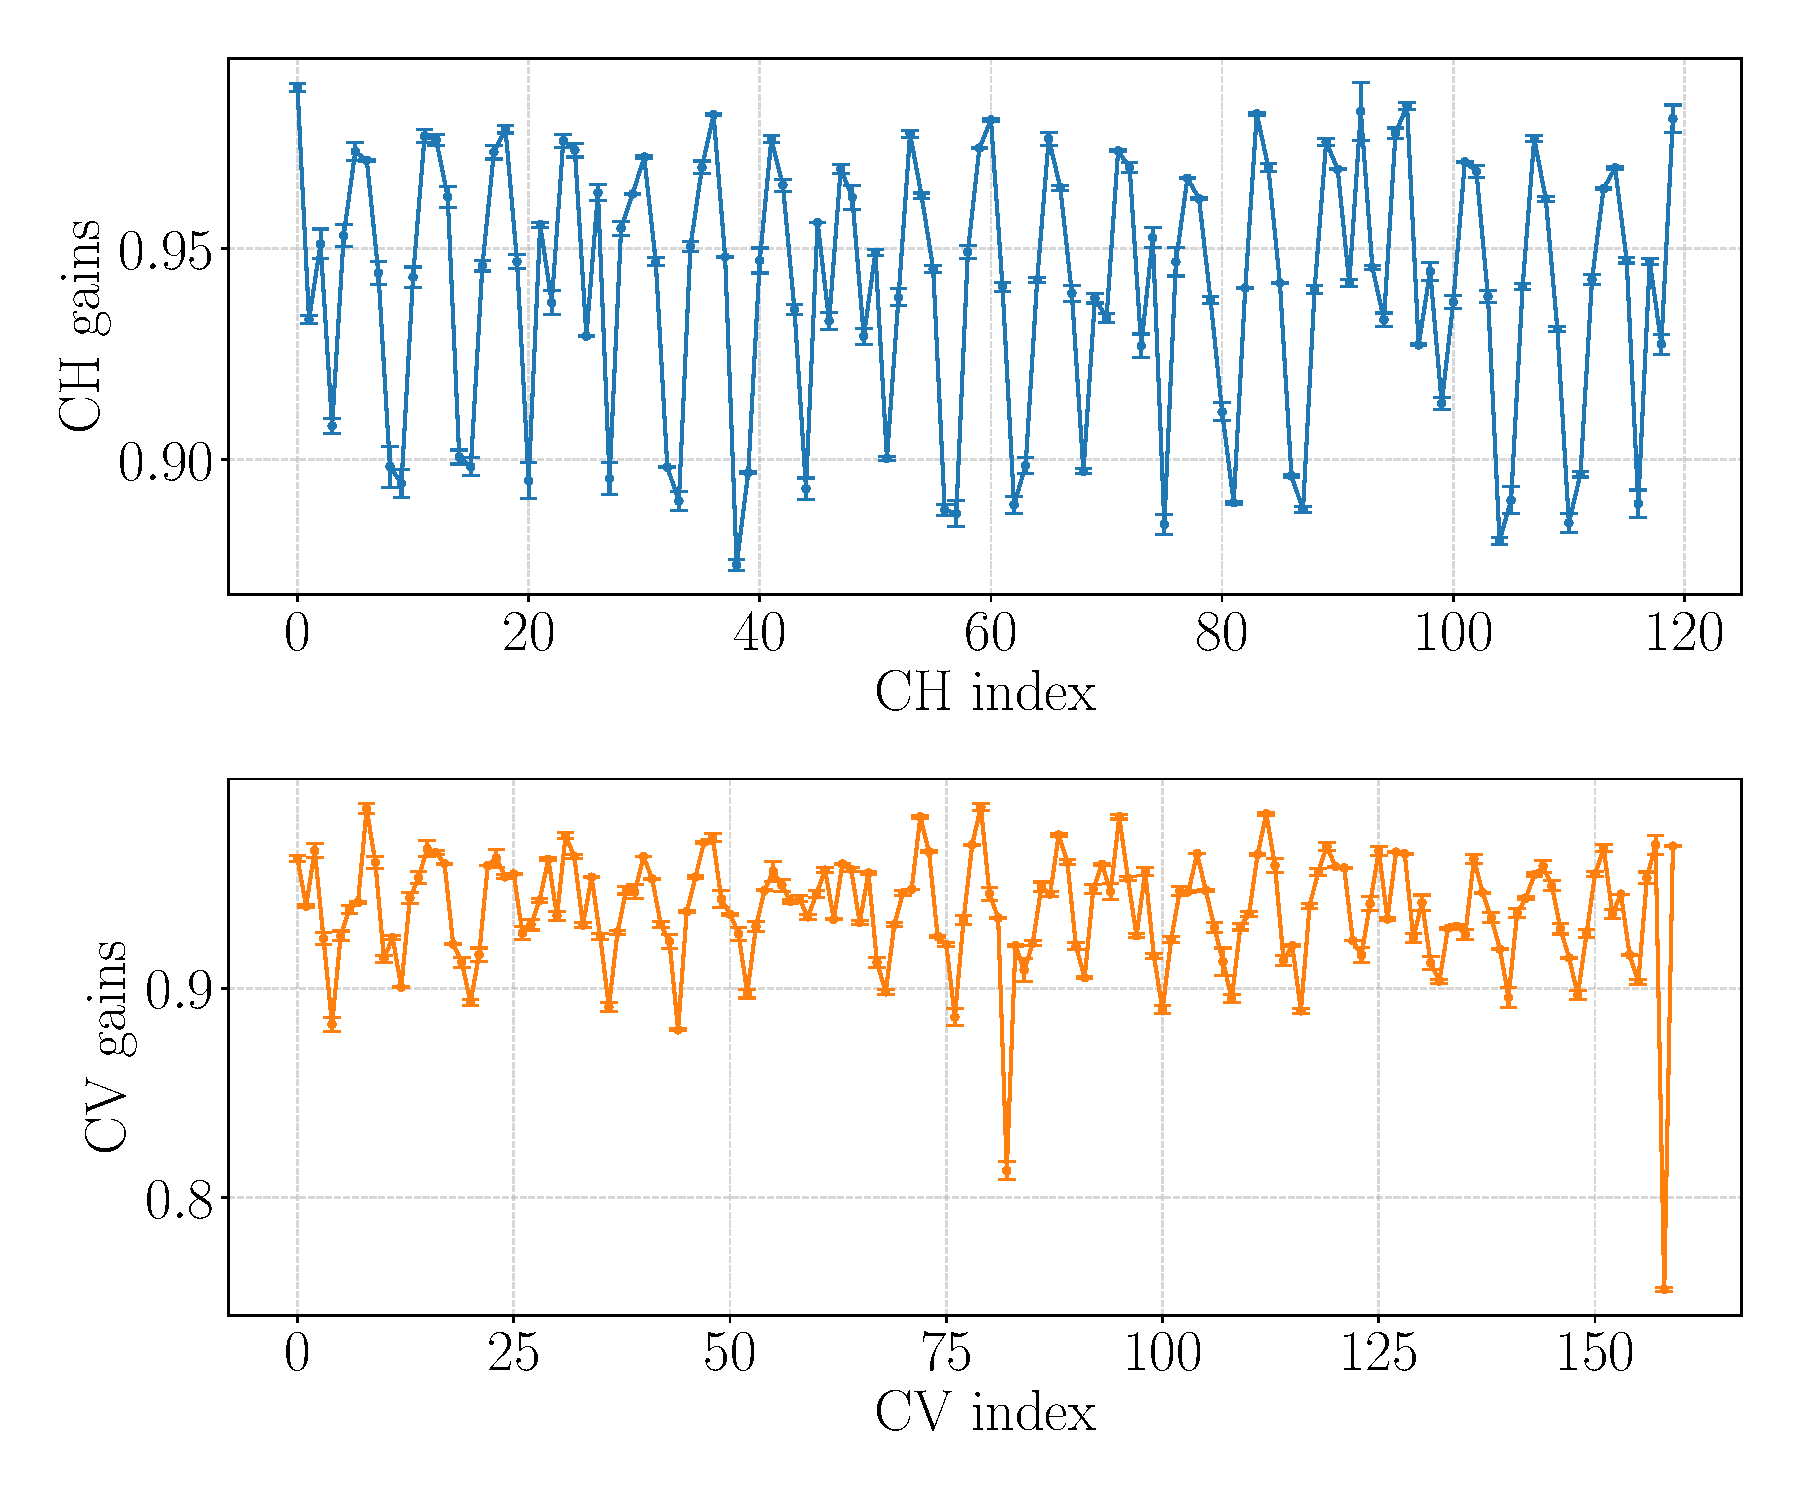
\includegraphics[width=1.0\textwidth]{figures/corr_gains_iter0_big.pdf}
    \caption{Correctors gains.}
    \label{subfig:corr_fit}
\end{subfigure}
\caption{Fitted values for BPM gains, roll errors and correctors (CH and CV) gains.}
\label{fig:gain_fit}
\end{figure}

The values in format (average $\pm$ std) for each parameter presented in Figure~\ref{fig:gain_fit} are: $\num{0.966(7)}$ for horizontal BPM gain, $\num{0.973(8)}$ for vertical BPM gain, $\num{0.94(3)}$ for CH gain, $\num{0.94(4)}$ for CV gain and $\SI{-1(3)}{\milli\radian}$ for BPM roll error. As discussed in Appendix~\ref{appendix:gains}, it was defined that the interpretations for BPM and correctors gains are opposite, in the sense that for BPMs the fitted gains represents the corrections factors that should be applied in the measurements to explain correctly the actual orbit distortions, while it is the inverse of correctors gains that should be used in the kicks applied to obtain the actual kicks that affected the beam. Therefore, this fitting indicates that the actual BPMs measurements are around $3\%$ lower than the actual values and the actual kicks that distort the beam orbit are $6\%$ greater than the kicks variations ($\SI{15}{\micro\radian}$) considered by the control system during~\gls{orm} measurement. It also can be observed that the spread between BPM gains is one order of magnitude lower than the spread between correctors and this difference was already expected.

In Figure~\ref{subfig:corr_fit} it can be observed a 20-fold periodic pattern in correctors gains. This signature following the storage ring period is also correlated to the topic of Section~\ref{sec:orbit_effect}. It also can be seen two outliers in CV gains in 82\ts{th} and 158\ts{th} vertical correctors. These correctors were later examined on site but this initial survey did not reveal any anomaly. The cause for these outliers in CV gains is still under investigation and they did not compromise the following results.

As already mentioned, the fitted gains obtained from the first LOCO iteration and presented in Figure~\ref{fig:gain_fit} were used as initial values for the following iterations. For this study, the obtained values were not used in the control system to correct the BPM measurements nor the correctors excitation curves. This was decided since the fitted gains are close to unity and they do not compromise greatly the orbit correction system and the~\gls{orm} measurement. For machine studies in the future, when much finer tuning in the storage ring and control system will be performed, the fitted gains and roll errors may also be included as correction factors for BPMs and correctors.

\subsection{Quadrupoles Gradients}
Normal and skew gradients were also included as LOCO fit parameters to adjust the measured~\gls{orm}. The normal gradients are associated to the corrections that can be applied in 270 quadrupoles trim-coils in Sirius storage ring and skew gradients to the 80 skew quadrupoles coils installed in sextupoles magnets.

The LOCO fitting changes the quadrupole gradients in the model to calibrate the measured ORM, so the integrated gradients are changed by $\mathrm{KL}_{\mathrm{nominal}} \rightarrow \mathrm{KL}_{\mathrm{nominal}} + \Delta\mathrm{KL}_{\mathrm{LOCO}}$. The same is valid for $\mathrm{KsL}$, the skew gradients strength, however the difference is that initially the skew gradients are zero, since in the nominal model the coupling is zero as well. Ideally, $\mathrm{KL}_{\mathrm{actual}} = \mathrm{KL}_{\mathrm{nominal}} + \Delta\mathrm{KL}_{\mathrm{LOCO}}$ represents the actual focusing strengths affecting the electron beam in the actual storage ring. Once the parameters of the real machine are calibrated, we are able to correct it to correspond to the nominal model or any other model of interest. In this way, it is possible to calculate the corrections that change the focusing strengths along the real storage ring to produce a linear optics close to the nominal.

The process of measuring an~\gls{orm}, fitting it with LOCO and applying the corrections to the machine was realized only twice and the convergence was reached. The corrections distribution history both for normal quadrupoles and skew quadrupoles are shown in Figure~\ref{fig:loco_corrections}. The standard deviations of these corrections for each LOCO iteration are organized in Table~\ref{tab:corr_converge}.
\begin{figure}
\centering
\begin{subfigure}[t]{1.0\textwidth}
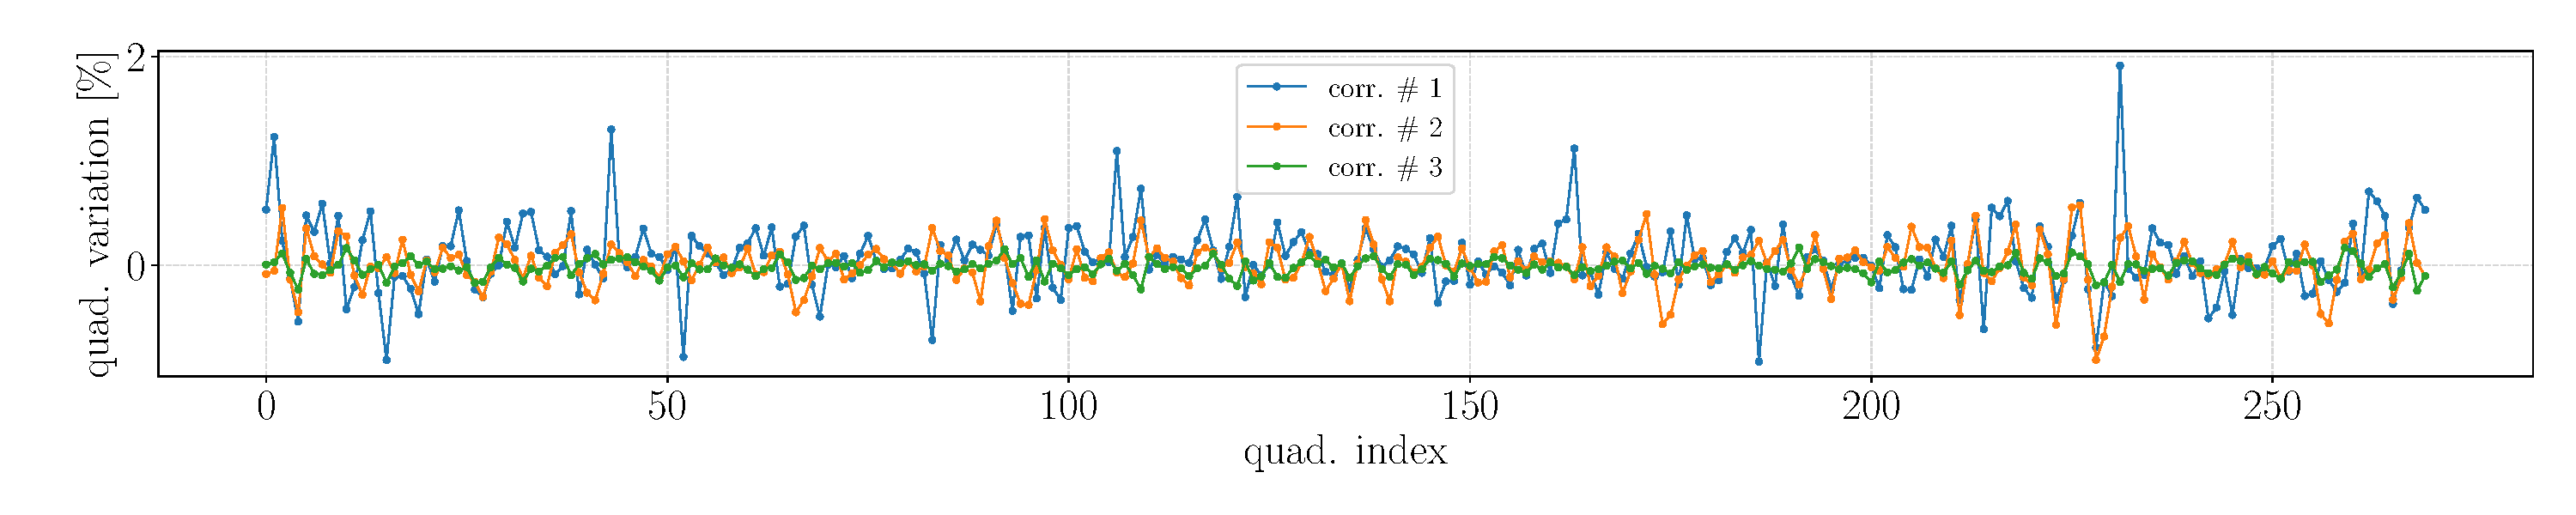
\includegraphics[width=1.0\textwidth]{figures/loco_quad_big.pdf}
    \caption{Quadrupoles trim-coils.}
    \label{subfig:quad_fit}
\end{subfigure}
 \begin{subfigure}[t]{1.0\textwidth}
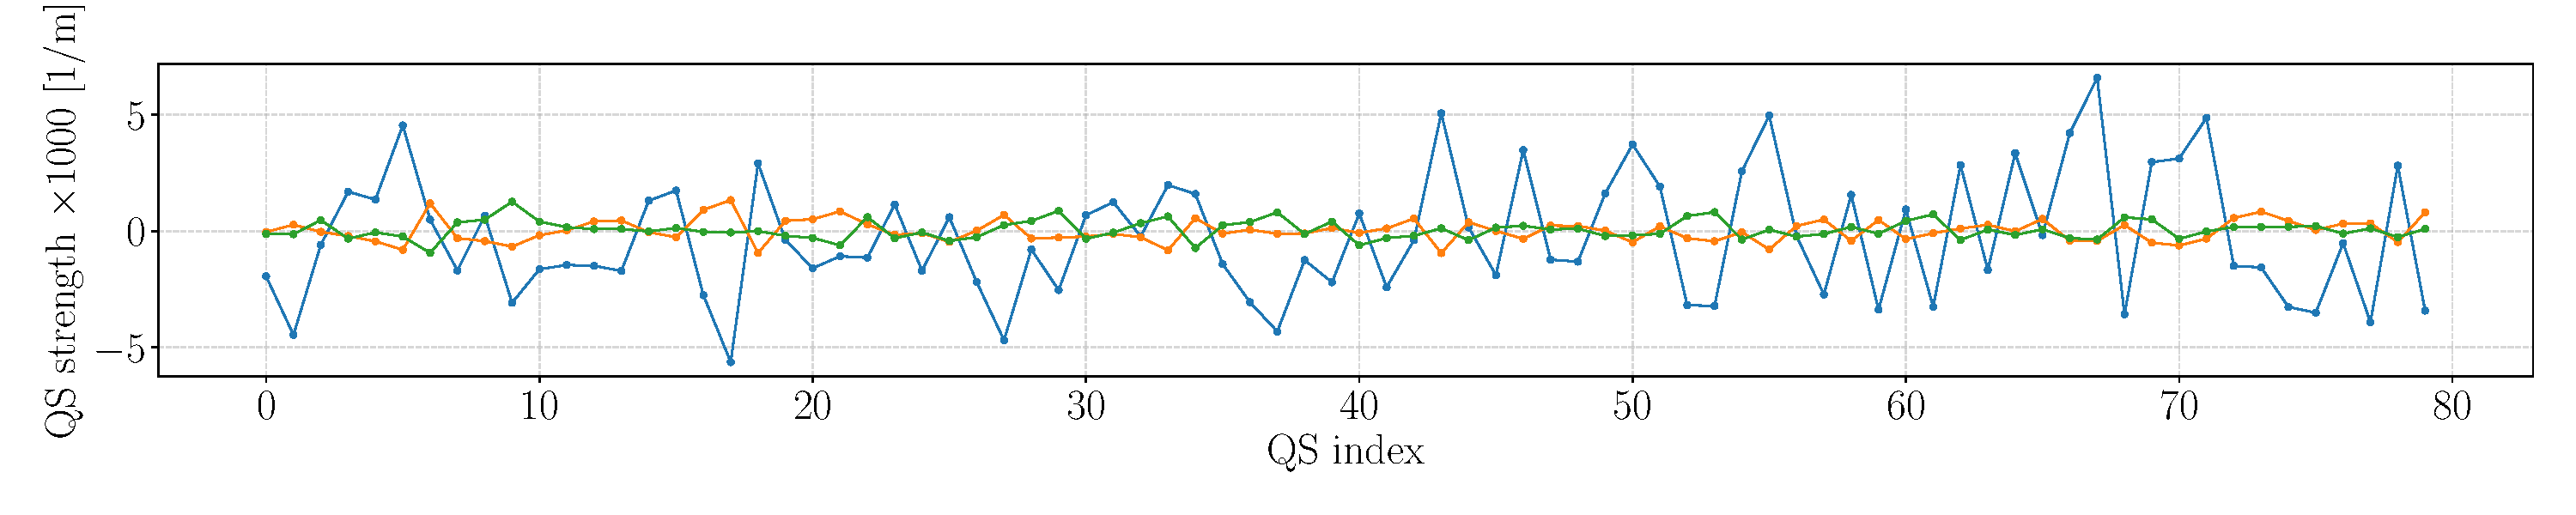
\includegraphics[width=1.0\textwidth]{figures/loco_qs_big.pdf}
    \caption{Skew quadrupoles.}
    \label{subfig:qs_fit}
\end{subfigure}
\caption{Normal and skew quadrupoles strength variations throughout LOCO iterations.}
\label{fig:loco_corrections}
\end{figure}
\begin{table}
    \centering
    \caption{Corrections strengths variation for each LOCO iteration.}
    \label{tab:corr_converge}
    \begin{tabular}{ccccc}
        \toprule\toprule
        Knobs variation (std) & corr. \#1 & corr. \#2 & corr. \#3 & Unit \\
        \hline
        Quadrupoles & \num{0.33} & \num{0.21} & \num{0.07} &\SI{}{\%}\\
        Skew Quadrupoles & \num{2.7e-3} & \num{5e-4} & \num{4e-4} & \SI{}{\meter^{-1}} \\
        \bottomrule\bottomrule
    \end{tabular}
\end{table}

From Figure~\ref{fig:loco_corrections} and the values in Table~\ref{tab:corr_converge} it can be seen that the corrections calculated in the third LOCO iteration and the respective parameters variations obtained, presented in Table~\ref{tab:fit_var}, are commensurable. Therefore, it was considered that in the third set of corrections the process already converged and this last set was not applied. 
% \begin{figure}
% \centering
% \begin{subfigure}[t]{0.49\textwidth}
% 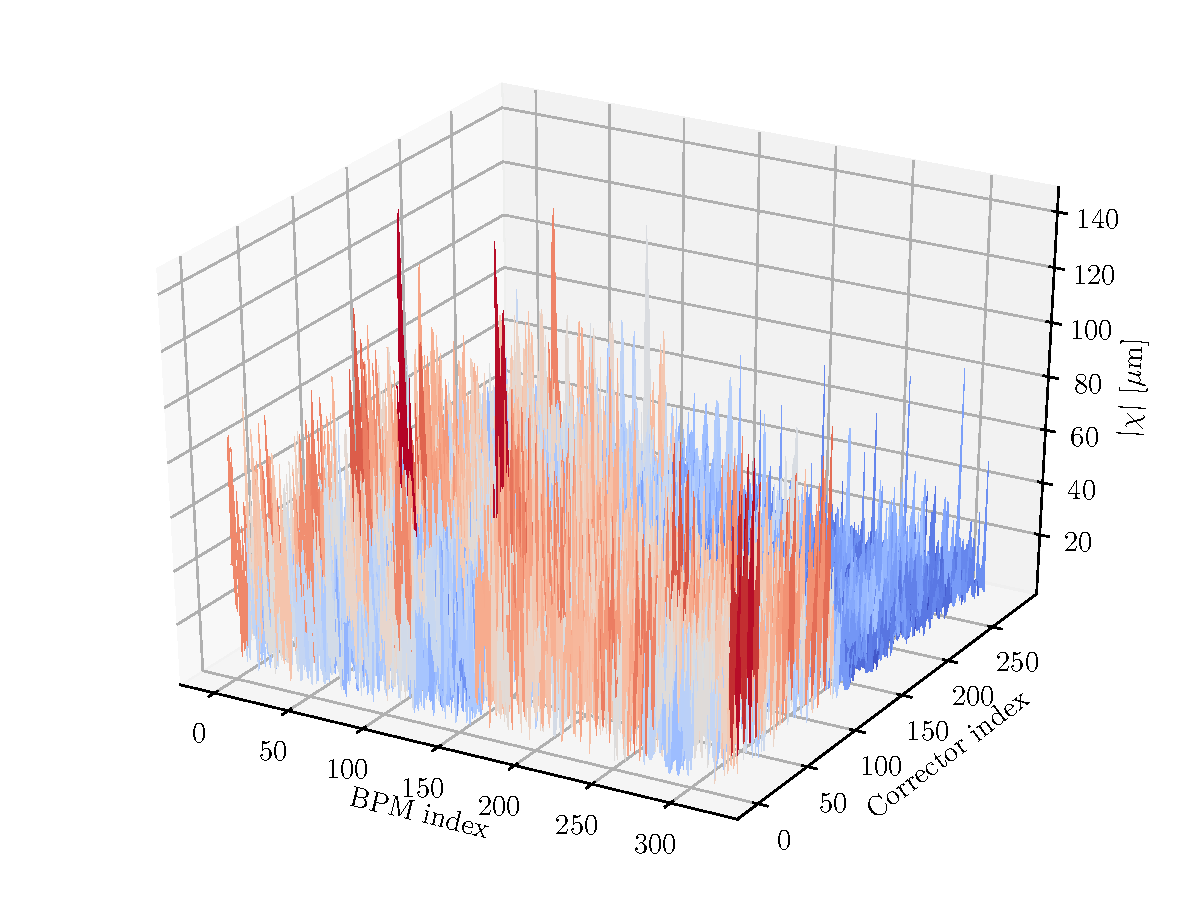
\includegraphics[width=1.0\textwidth]{figures/surface_before_loco.pdf}
%     \caption{Before.}
%     \label{subfig:ondiag}
% \end{subfigure}
%  \begin{subfigure}[t]{0.49\textwidth}
% 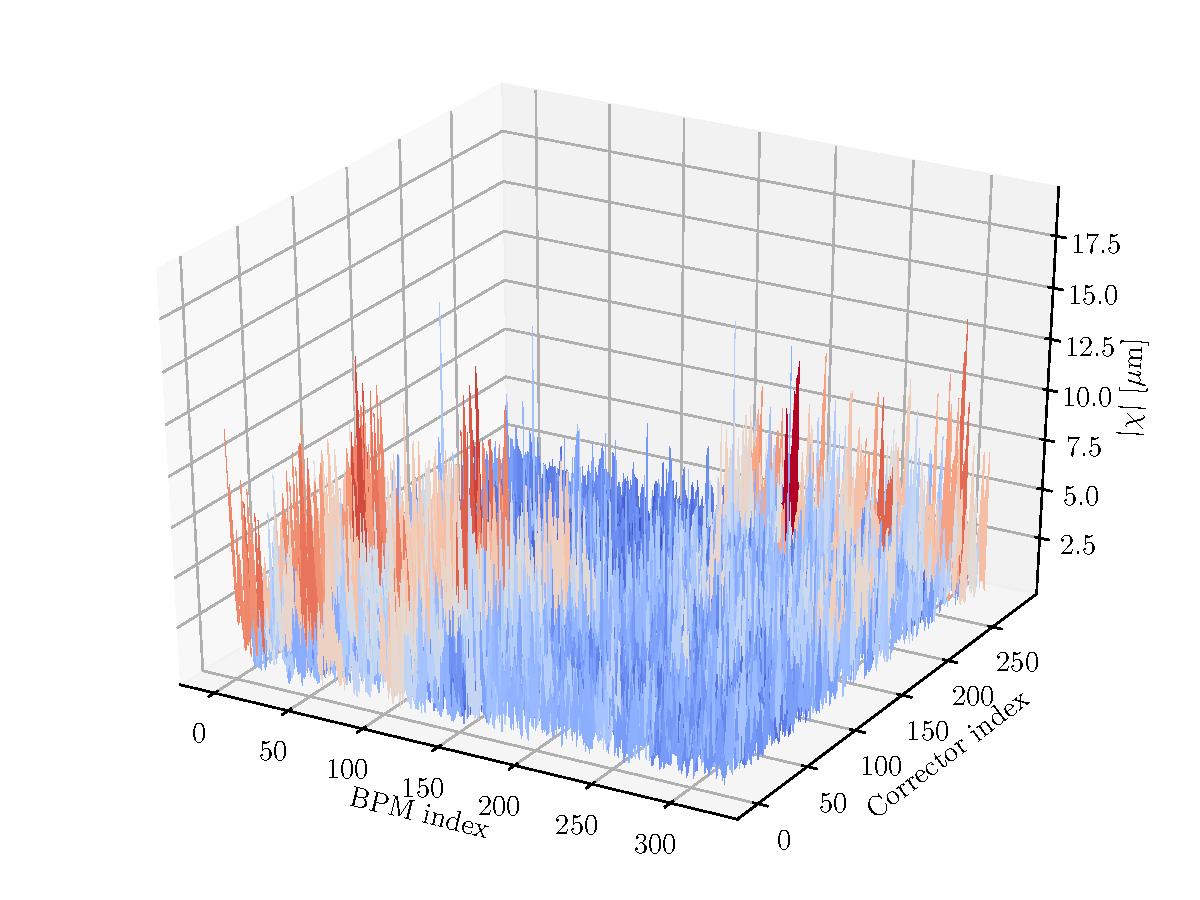
\includegraphics[width=1.0\textwidth]{figures/surface_after_loco.pdf}
%     \caption{After.}
%     \label{subfig:offdiag}
% \end{subfigure}
% \caption{Orbit response matrix error surface before and after LOCO corrections.}
% \label{fig:hist}
% \end{figure}

\subsection{Deviations from Nominal}
The figure of merit to be minimized with LOCO method is the difference between measured and calculated~\gls{orm} in each iteration, by changing the storage ring model. As LOCO corrections are applied in the machine elements, it is expected that the measured~\gls{orm} converges to the nominal~\gls{orm}. Table~\ref{tab:orm_progress} shows the progress of~\gls{orm} differences (represented by $\chi$) throughout LOCO corrections applied to the machine and also the fitting level for each particular iteration.
\begin{table}
    \centering
    \caption{ORM fitting progress.}
    \label{tab:orm_progress}
    \begin{tabular}{ccc}
        \toprule\toprule
        LOCO iteration & Initial $\chi$ [$\SI{}{\micro\meter}$] & Final $\chi$ [$\SI{}{\micro\meter}$] \\
        \hline
        \#1 & 24.6 & 0.94 \\
        \#2 & 2.7 & 0.90 \\
        \#3 & 2.1 & 0.92 \\
        \bottomrule\bottomrule
    \end{tabular}
\end{table}

The LOCO corrections applied to Sirius storage ring decreased the difference between measured and nominal~\gls{orm} from $\SI{24.6}{\micro\meter}$ to $\SI{2.1}{\micro\meter}$, which is almost a factor $12$ of reduction.

For a global view of measured~\gls{orm} convergence towards the nominal, Figure~\ref{fig:histogram} shows the histogram of errors for each LOCO iteration. The error histograms are divided in four parts, following the four~\gls{orm} blocks: $M_{xx}$, $M_{yy}$ (diagonal) and $M_{xy}$, $M_{yx}$ (off-diagonal). 
\begin{figure}
\centering
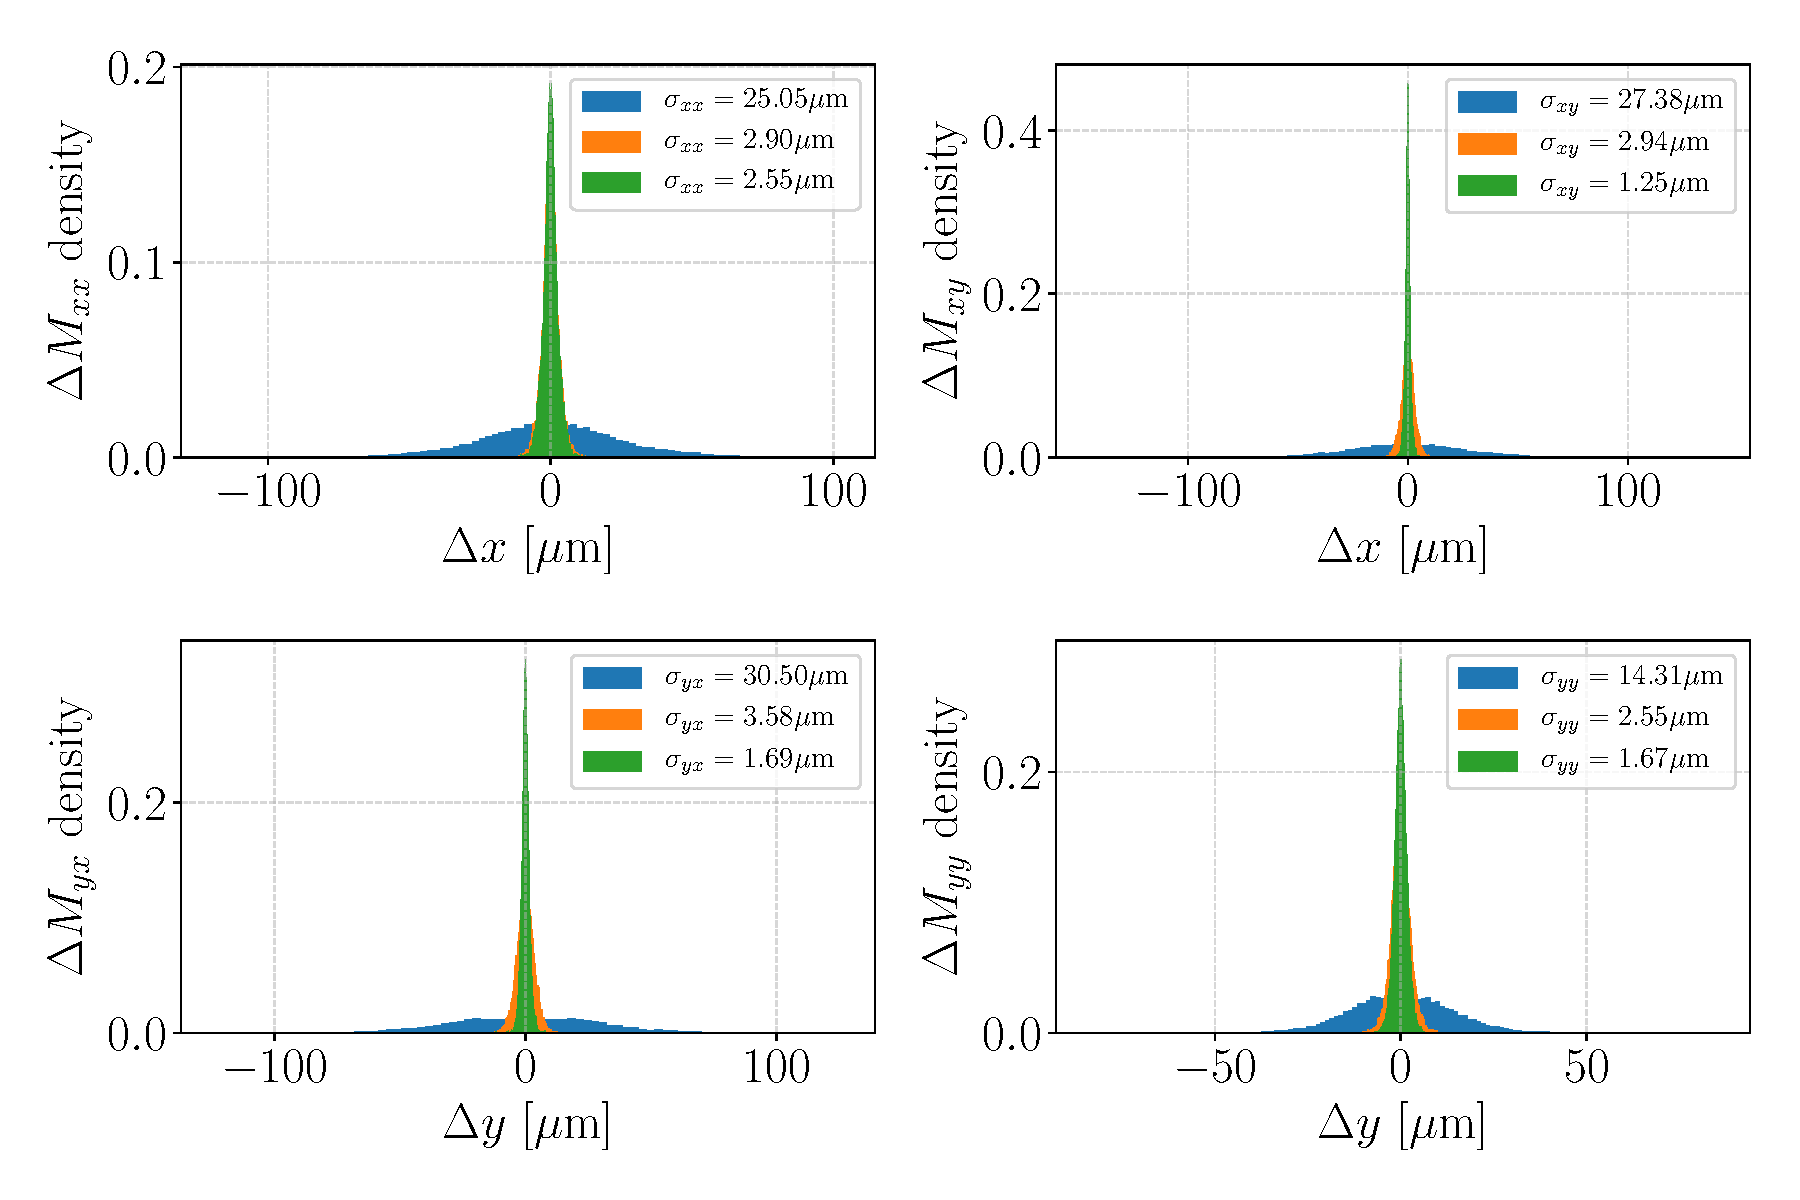
\includegraphics[width=1.0\textwidth]{figures/histogram_loco_iterations3_density.pdf}
\caption{Histogram for the errors between measured and nominal orbit response matrices for each LOCO iteration. The blue data refers to the measured ORM without corrections applied. The orange data was obtained after the first application of LOCO corrections. The green data is related to the second and last LOCO round applied.}
\label{fig:histogram}
\end{figure}

It can be seen that initially the order of magnitude of errors are basically the same for all blocks. The off-diagonal errors (related to coupling errors) are slightly greater than the diagonal errors. After the first correction application in the storage ring, the errors in the four blocks were already greatly reduced. After the second and final corrections the~\gls{std} errors were reduced by the following factors: 
\begin{align*}
    \sigma_{xx}^{\mathrm{initial}}/\sigma_{xx}^{\mathrm{final}} = 9.8, & \hspace{1.5cm} \sigma_{xy}^{\mathrm{initial}}/\sigma_{xy}^{\mathrm{final}} = 21.9, \\
    \sigma_{yx}^{\mathrm{initial}}/\sigma_{yx}^{\mathrm{final}} = 18.0, & \hspace{1.5cm}
    \sigma_{yy}^{\mathrm{initial}}/\sigma_{yy}^{\mathrm{final}} = 8.6. 
\end{align*}

The off-diagonal errors were reduced by a factor of 2 greater than the diagonal errors.

Two~\gls{orm} columns were taken to exemplify typical differences between measured and nominal matrices, before and after LOCO corrections and the results are presented in Figure~\ref{fig:orm_rows}. The first column is related to a horizontal corrector signature and the second one to a vertical corrector. Multiplying the~\gls{orm} columns by the kicks $\Delta\theta_x$ and $\Delta\theta_y$, one can obtain the orbit distortion signature $\Delta x$ and $\Delta y$.
\begin{figure}
\centering
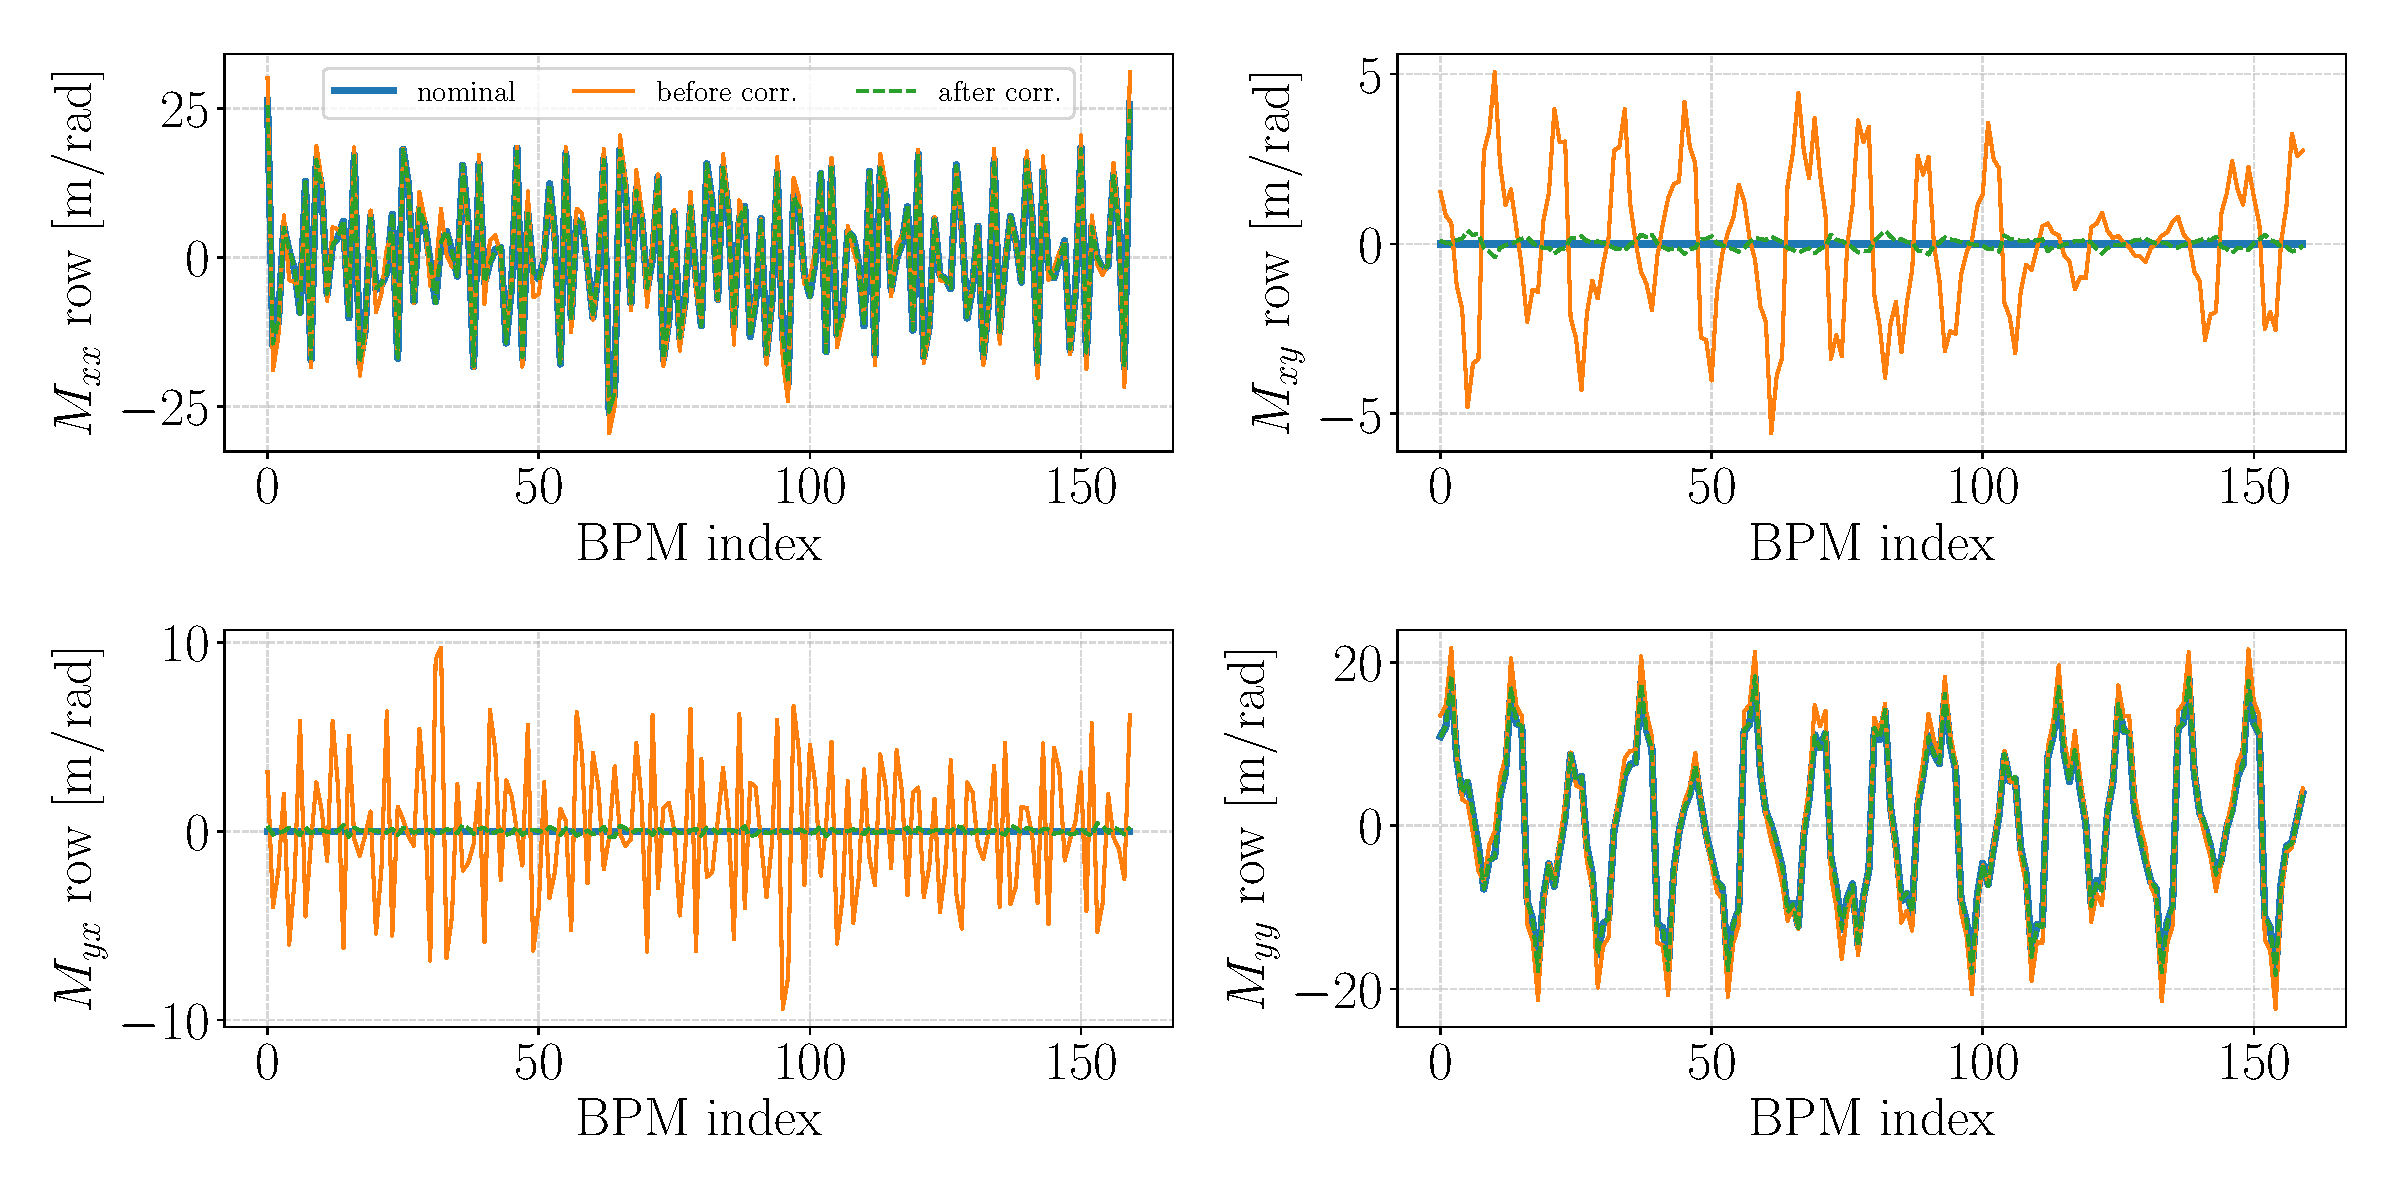
\includegraphics[width=1.0\textwidth]{figures/nominal_measured_after_before_loco_big.pdf}
\caption{ORM rows for the first CH and CV. The blue curve is the nominal ORM, the orange curve represents the measured ORM before LOCO corrections and the green curve is from measured ORM after LOCO.}
\label{fig:orm_rows}
\end{figure}

In this example it can be seen that the off-diagonal elements are greatly reduced and are close to zero after corrections. The diagonal elements for measured and nominal~\gls{orm} are practically overlapped.

\subsection{Final Corrections}
Adding up the corrections sets for normal and skew quadruploles gradients in the two LOCO iterations, the total corrections were obtained and plotted in Figure~\ref{fig:loco_corrections_final}.
\begin{figure}
\centering
\begin{subfigure}[t]{1.0\textwidth}
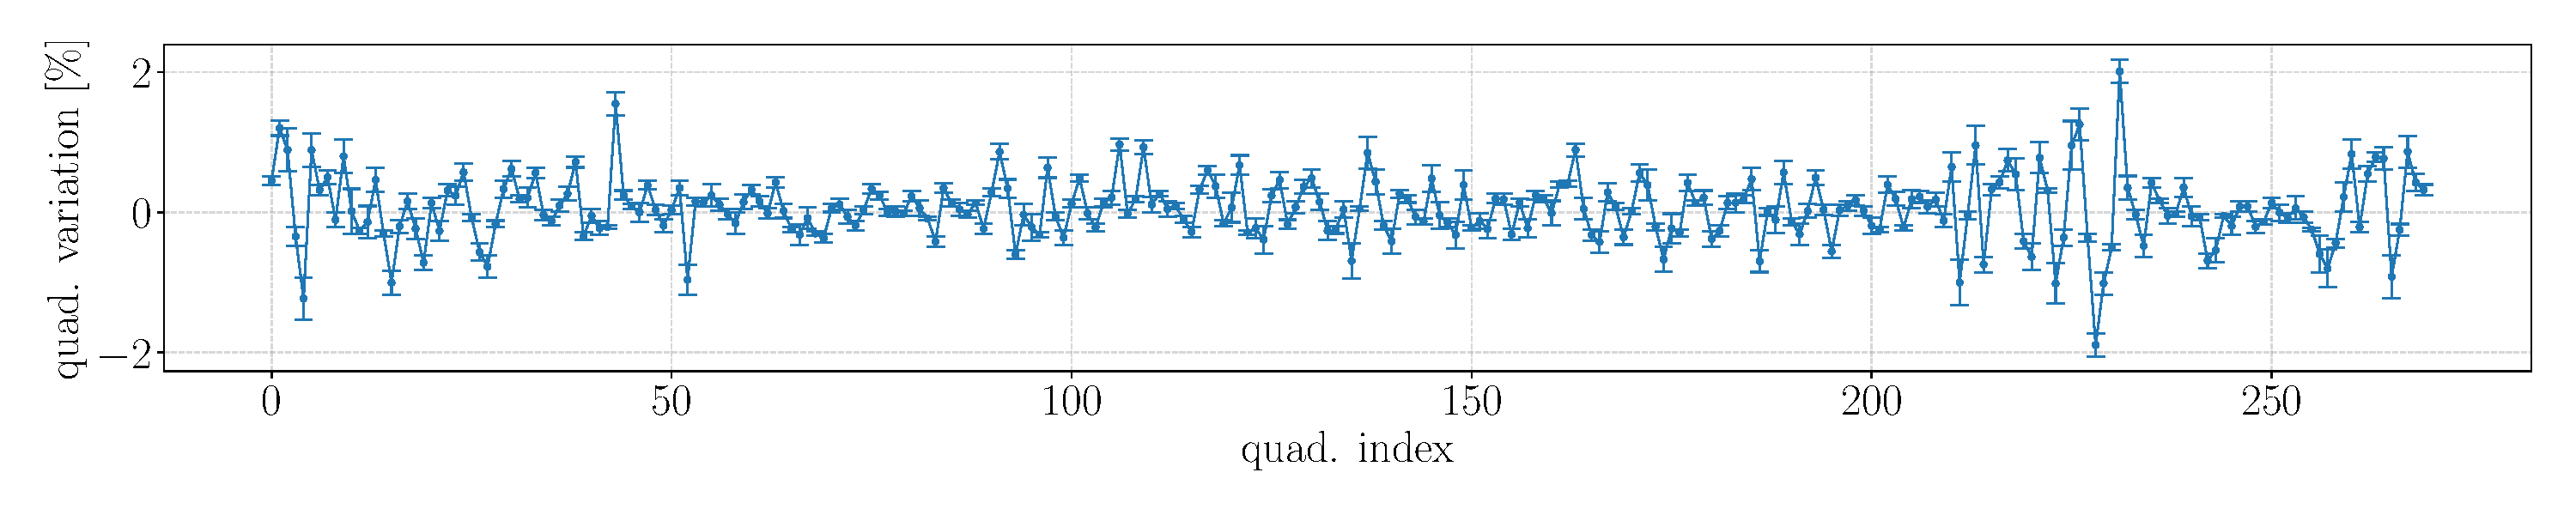
\includegraphics[width=1.0\textwidth]{figures/loco_quad_corrections_errorbar_big.pdf}
    \caption{Quadrupoles trim-coils.}
    \label{subfig:quad_fit_final}
\end{subfigure}
 \begin{subfigure}[t]{1.0\textwidth}
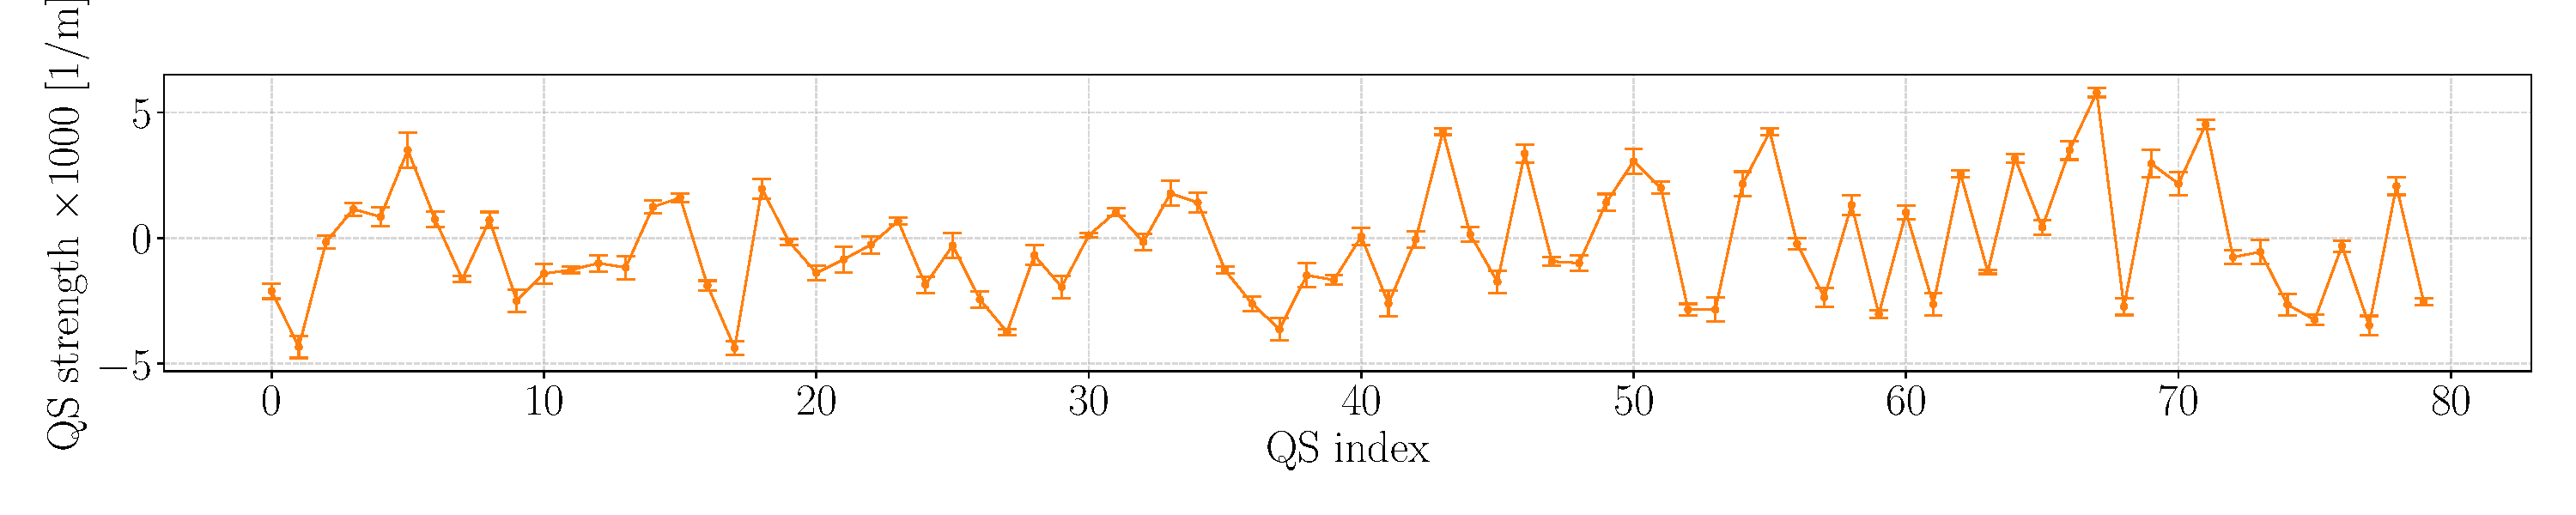
\includegraphics[width=1.0\textwidth]{figures/loco_qs_corrections_errorbar_big.pdf}
    \caption{Skew quadrupoles.}
    \label{subfig:qs_fit_final}
\end{subfigure}
\caption{Normal and skew quadrupoles final corrections.}
\label{fig:loco_corrections_final}
\end{figure}

The final quadrupole gradients variations covers the range of $\pm 2\%$, while the skew quadrupole strengths are between $\pm \SI{5e-3}{\meter^{-1}}$. Based only on magnetic characterization of quadrupoles fields, variations of $2\%$ are large, since the specifications for gradient errors were $0.05\%$. On the other hand, it is important to remember that these quadrupole variations are corrections for gradient errors along the whole storage ring. Thus, it is more likely that these corrections are compensating for other sources of gradient errors. The most important contribution is additional fields in quadrupoles and sextupoles caused by the feed-down effect (Appendix~\ref{appendix:feed-down} for details) due to magnet misalignment and orbit distortions. These other sources of gradient errors may accumulate in such a way that quadrupole variations on the order of $2\%$ might be necessary for compensation.

An interesting way to visualize the quadrupole variations is dividing them following the 12 quadrupoles families in storage ring. The magnets that make up each family were selected to minimize the spread in gradient strengths within the families and to satisfy the $0.05\%$ specification on gradient errors. The results of this rearrangement in families are shown in Figure~\ref{fig:loco_corrections_final_families}. The statistics for these quadrupole variations divided by families are organized in Table~\ref{tab:quad_fam_corr}.
\begin{figure}
\centering
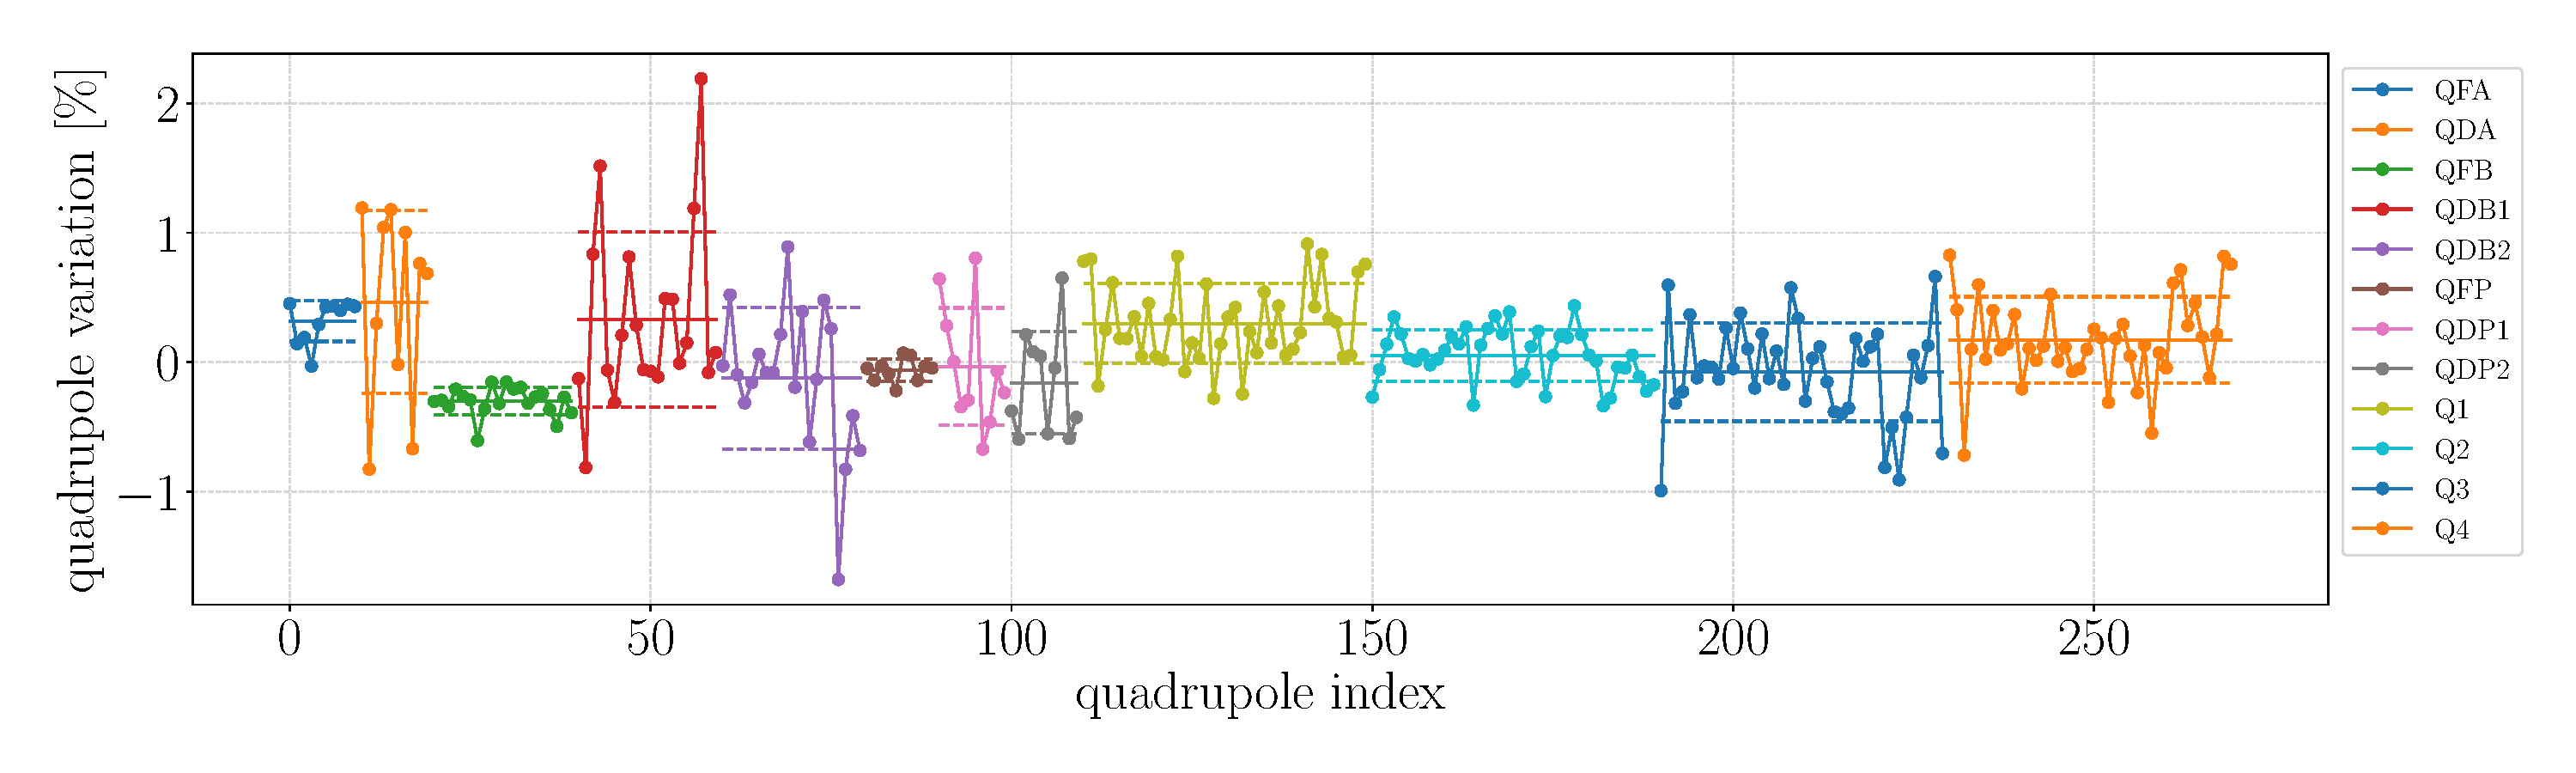
\includegraphics[width=1.0\textwidth]{figures/final_quads_correction_families_fix.pdf}
\caption{Quadrupoles families final variations after two LOCO iterations. The continuous lines indicate the family average variation and the dashed lines correspond to $\pm$ std.}
\label{fig:loco_corrections_final_families}
\end{figure}
\begin{table}
    \centering
    \caption{Quadrupole families corrections.}
    \label{tab:quad_fam_corr}
    \begin{tabular}{cccc}
        \toprule\toprule
        Quad. Family & mean [\%] & std [\%] & peak-to-valley [\%] \\
        \hline
        QDA  &  0.45  & 0.71 & 2.02 \\
        QDB1 &  0.31  & 0.68 & 3.00 \\
        QDB2 &  -0.14 &  0.55&  2.57 \\
        QDP1 &  -0.05 &  0.45 &  1.48 \\
        QDP2 &  -0.18 &  0.39 &  1.25 \\
        \hline
        QFA  &  0.31  & 0.16 & 0.48 \\
        Q1   &  0.30  & 0.31 & 1.19 \\
        Q2   &  0.05  & 0.20 & 0.77 \\
        Q3   &  -0.08 &  0.38 &  1.66 \\
        Q4   &  0.17  & 0.33 & 1.55 \\
        \hline
        QFB  &  -0.31 & 0.11 &  0.45 \\
        QFP  &  -0.07 &  0.08 &   0.29 \\
        \bottomrule\bottomrule
    \end{tabular}
\end{table}

Mechanically, three types of quadrupoles were used in Sirius storage ring, namely Q14, Q20 and Q30. The number in the name indicates the magnet length, $\SI{14}{\cm}$, $\SI{20}{\cm}$ and $\SI{30}{\cm}$, respectively. The shorter quadrupoles, Q14, were used as defocusing quadrupoles. Q20 were used as quadrupoles in arc sections and for focusing quadrupoles in high-beta straight sections. The longest quadrupoles, Q30, were used as focusing quadrupoles in low-beta sections, in order to provide a larger integrated gradient field to focus the betatron functions in the straight sections. The quadrupole families information in Table~\ref{tab:quad_fam_corr} are divided with horizontal line into three groups, following each magnet type to which each corresponding family. 

For Sirius quadrupoles, the integrated gradient strength increases with the quadrupole length. Suppose that the variations $\Delta \mathrm{KL}$ calculated with LOCO are on the same order of magnitude for all quadrupoles. Thus, the relative change $\Delta \mathrm{KL}/ \mathrm{KL}$ is smaller as the quadrupole's integrated gradient is larger, as can be confirmed in Table~\ref{tab:quad_fam_corr}. This indicates that there is no systematic problems in specific quadrupoles types and families. 
% It can be observed that Q30 quadrupoles, QFB and QFP, presented the smaller variations, followed by Q20 and Q14 types, which are the defocusing quadrupoles, presented the largest variations. At the time of writing, the reason for these differences was not clearly understood. The LNLS Magnet Group were performing new magnetic characterizations and analysis with the quadrupoles available in the measurement laboratory to investigate the question in collaboration with LNLS~\gls{fac}.

\subsection{Calibrated Model Parameters}
Once the measured~\gls{orm} is adjusted, with the obtained calibrated model one can calculate lattice functions (beta and dispersion), and global parameters, such as betatron tunes and emittances. If the model describes accurately the real machine, this provides an indirect estimate of corresponding actual parameters.

A function that is related to the storage ring linear optics errors and asymmetries is the betatron function relative error $\Delta \beta(s)/\beta(s)$, called beta-beating. The beta-beating is a $s$-dependent function but it is common to use its standard deviation value as a characteristic parameter for the optics errors level. The dispersion function~\gls{std} deviation from nominal values is an usual parameter to indicate the optics error as well. In Table~\ref{tab:calibrated_optics}, the~\gls{std} values for beta-beating and dispersion errors are shown for each of the LOCO fits.
\begin{table}
    \centering
    \caption{Lattice functions errors from calibrated model throughout LOCO fittings.}
    \label{tab:calibrated_optics}
    \begin{tabular}{ccccc}
        \toprule\toprule
        Parameter (std) & fitting \#1 & fitting \#2 & fitting \#3 & Unit \\
        \hline
        $\Delta\beta_x/\beta_x$ & \num{11.2} & \num{1.3} & \num{1.1} &\SI{}{\%}  \\
        $\Delta\beta_y/\beta_y$ & \num{7.9} & \num{0.9} & \num{1.6} &\SI{}{\%} \\
        $\Delta\eta_x$ &  \num{10.1} &  \num{1.6} & \num{1.4} & \SI{}{\milli\meter}  \\
        $\Delta\eta_y$ &  \num{3.1} &  \num{1.4} & \num{0.5} & \SI{}{\milli\meter} \\
        \bottomrule\bottomrule
    \end{tabular}
\end{table}

The results in Table~\ref{tab:calibrated_optics} indicate that $\Delta\beta_x/\beta_x$ in the calibrated models could have been reduced to one tenth of its initial value. $\Delta\beta_y/\beta_y$ was reduced by a factor 5. The reduction factors for horizontal and vertical dispersion errors were $7$ and $6$, respectively. However, independent measurements performed in the storage ring indicate that the actual error reductions were lower than predicted with LOCO models, as presented in the next section. 

From the calibrated model, the calculated fractional tunes agreed quite well with the measured ones as can be seen in Table~\ref{tab:calibrated_tunes}. The differences between the measured and predicted tunes from LOCO are on the order of $\num{1e-3}$ for both planes.
\begin{table}
    \centering
    \caption{Predicted fractional tunes from calibrated model compared to the measured ones for each LOCO fitting.}
    \label{tab:calibrated_tunes}
    \begin{tabular}{cccc}
        \toprule\toprule
        Parameter & fitting \#1 & fitting \#2 & fitting \#3 \\
        \hline
        measured $\nu_x$ & \num{0.076} & \num{0.076} & \num{0.076} \\
        model $\nu_x$ & \num{0.079} & \num{0.075} & \num{0.075}  \\
        % $|\Delta \nu_x|$ & \num{0.003} & \num{0.001} & \num{0.001}  \\
        \hline
        measured $\nu_y$ & \num{0.134} & \num{0.138} & \num{0.136} \\
        model $\nu_y$ & \num{0.135} & \num{0.137} & \num{0.133}  \\
        % $|\Delta \nu_y|$ & \num{0.001} & \num{0.001} & \num{0.003}  \\
        \bottomrule\bottomrule
    \end{tabular}
\end{table}

Finally, with the calibrated models the emittances were also calculated and the results are presented in Table~\ref{tab:calibrated_emittances}. Initially the model indicated that the natural emittance was $13\%$ higher than the nominal value of $\SI{251}{\pico\meter\radian}$. The vertical emittance generated an emittance coupling ratio of $0.94\%$. The natural emittance obtained with the final calibrated model was very close to the nominal and the vertical emittance was very close to zero.
\begin{table}
    \centering
    \caption{Emittances from calibrated model throughout LOCO fittings.}
    \label{tab:calibrated_emittances}
    \begin{tabular}{ccccc}
        \toprule\toprule
        Parameter & fitting \#1 & fitting \#2 & fitting \#3 & Unit \\
        \hline
        $\epsilon_0$ & \num{283.4} & \num{250.4} & \num{251.6} & \SI{}{\pico\meter\radian}  \\
        $\epsilon_x$ & \num{280.7} & \num{250.0} & \num{251.5} & \SI{}{\pico\meter\radian} \\
        $\epsilon_y$ &  \num{2.65} &  \num{0.37} & \num{0.07} & \SI{}{\pico\meter\radian}  \\
        $\epsilon_y/\epsilon_x$ &  \num{0.94} &  \num{0.15} & \num{0.03} & \SI{}{\%} \\
        \bottomrule\bottomrule
    \end{tabular}
\end{table}
\section{Independent Measurements}\label{sec:independent_meas}
Some measurements can be performed to check independently the impact of LOCO corrections on Sirius storage ring. Lattice functions, betatron and dispersion, are measured to verify the machine linear optics and its deviations from the nominal functions. Measuring the closest betatron tunes approximation provides information about the global betatron coupling. To check the performance in beam dynamics, one can measure the dynamic aperture and injection efficiency, two typically correlated quantities. When these studies were performed, the Sirius diagnostic beamline was not installed yet, so it was not possible to perform beam size and emittance measurements.

\subsection{Dispersion Function}
The information about dispersion function is already encoded in one of~\gls{orm} columns. A column of this matrix is the orbit response due to a variation in~\gls{rf} frequency. From Eq.~\eqref{eq:rf_column}, the dispersion function at the BPMs positions can be calculated as:
\begin{equation}
\eta_u(s_i) = -\alpha f_{\mathrm{rf}}\dfrac{\Delta u_i}{ \Delta f_{\mathrm{rf}}},
\end{equation}
where $u=x, y$ and $\alpha$ is the momentum compaction factor. Thus, given the~\gls{rf} frequency used in~\gls{orm} measurements, the dispersion is obtained with the corresponding~\gls{orm} column.

In this case, the dispersion function is not exactly an independent measurement, since it is included in LOCO fitting. For Sirius, it was required to include a weight factor to force the matching between measured and calculated dispersion function. It was verified that if this factor was not used, the measured~\gls{orm} was adjusted except for the dispersion column. Applying the gradients variations calculated by LOCO actually increased $\eta(s)$ errors, especially in the vertical plane. On the other hand, if the weight factor was further increased, the measured $\eta(s)$ was better explained with the model however the~\gls{orm} fitting quality was lowered.

With the measured~\gls{orm}s before and after LOCO corrections, $\eta_x$ and $\eta_y$ at~\glspl{bpm} were calculated and compared with the nominal function. The results are shown in Figure~\ref{fig:disp_error}. 
\begin{figure}
\centering
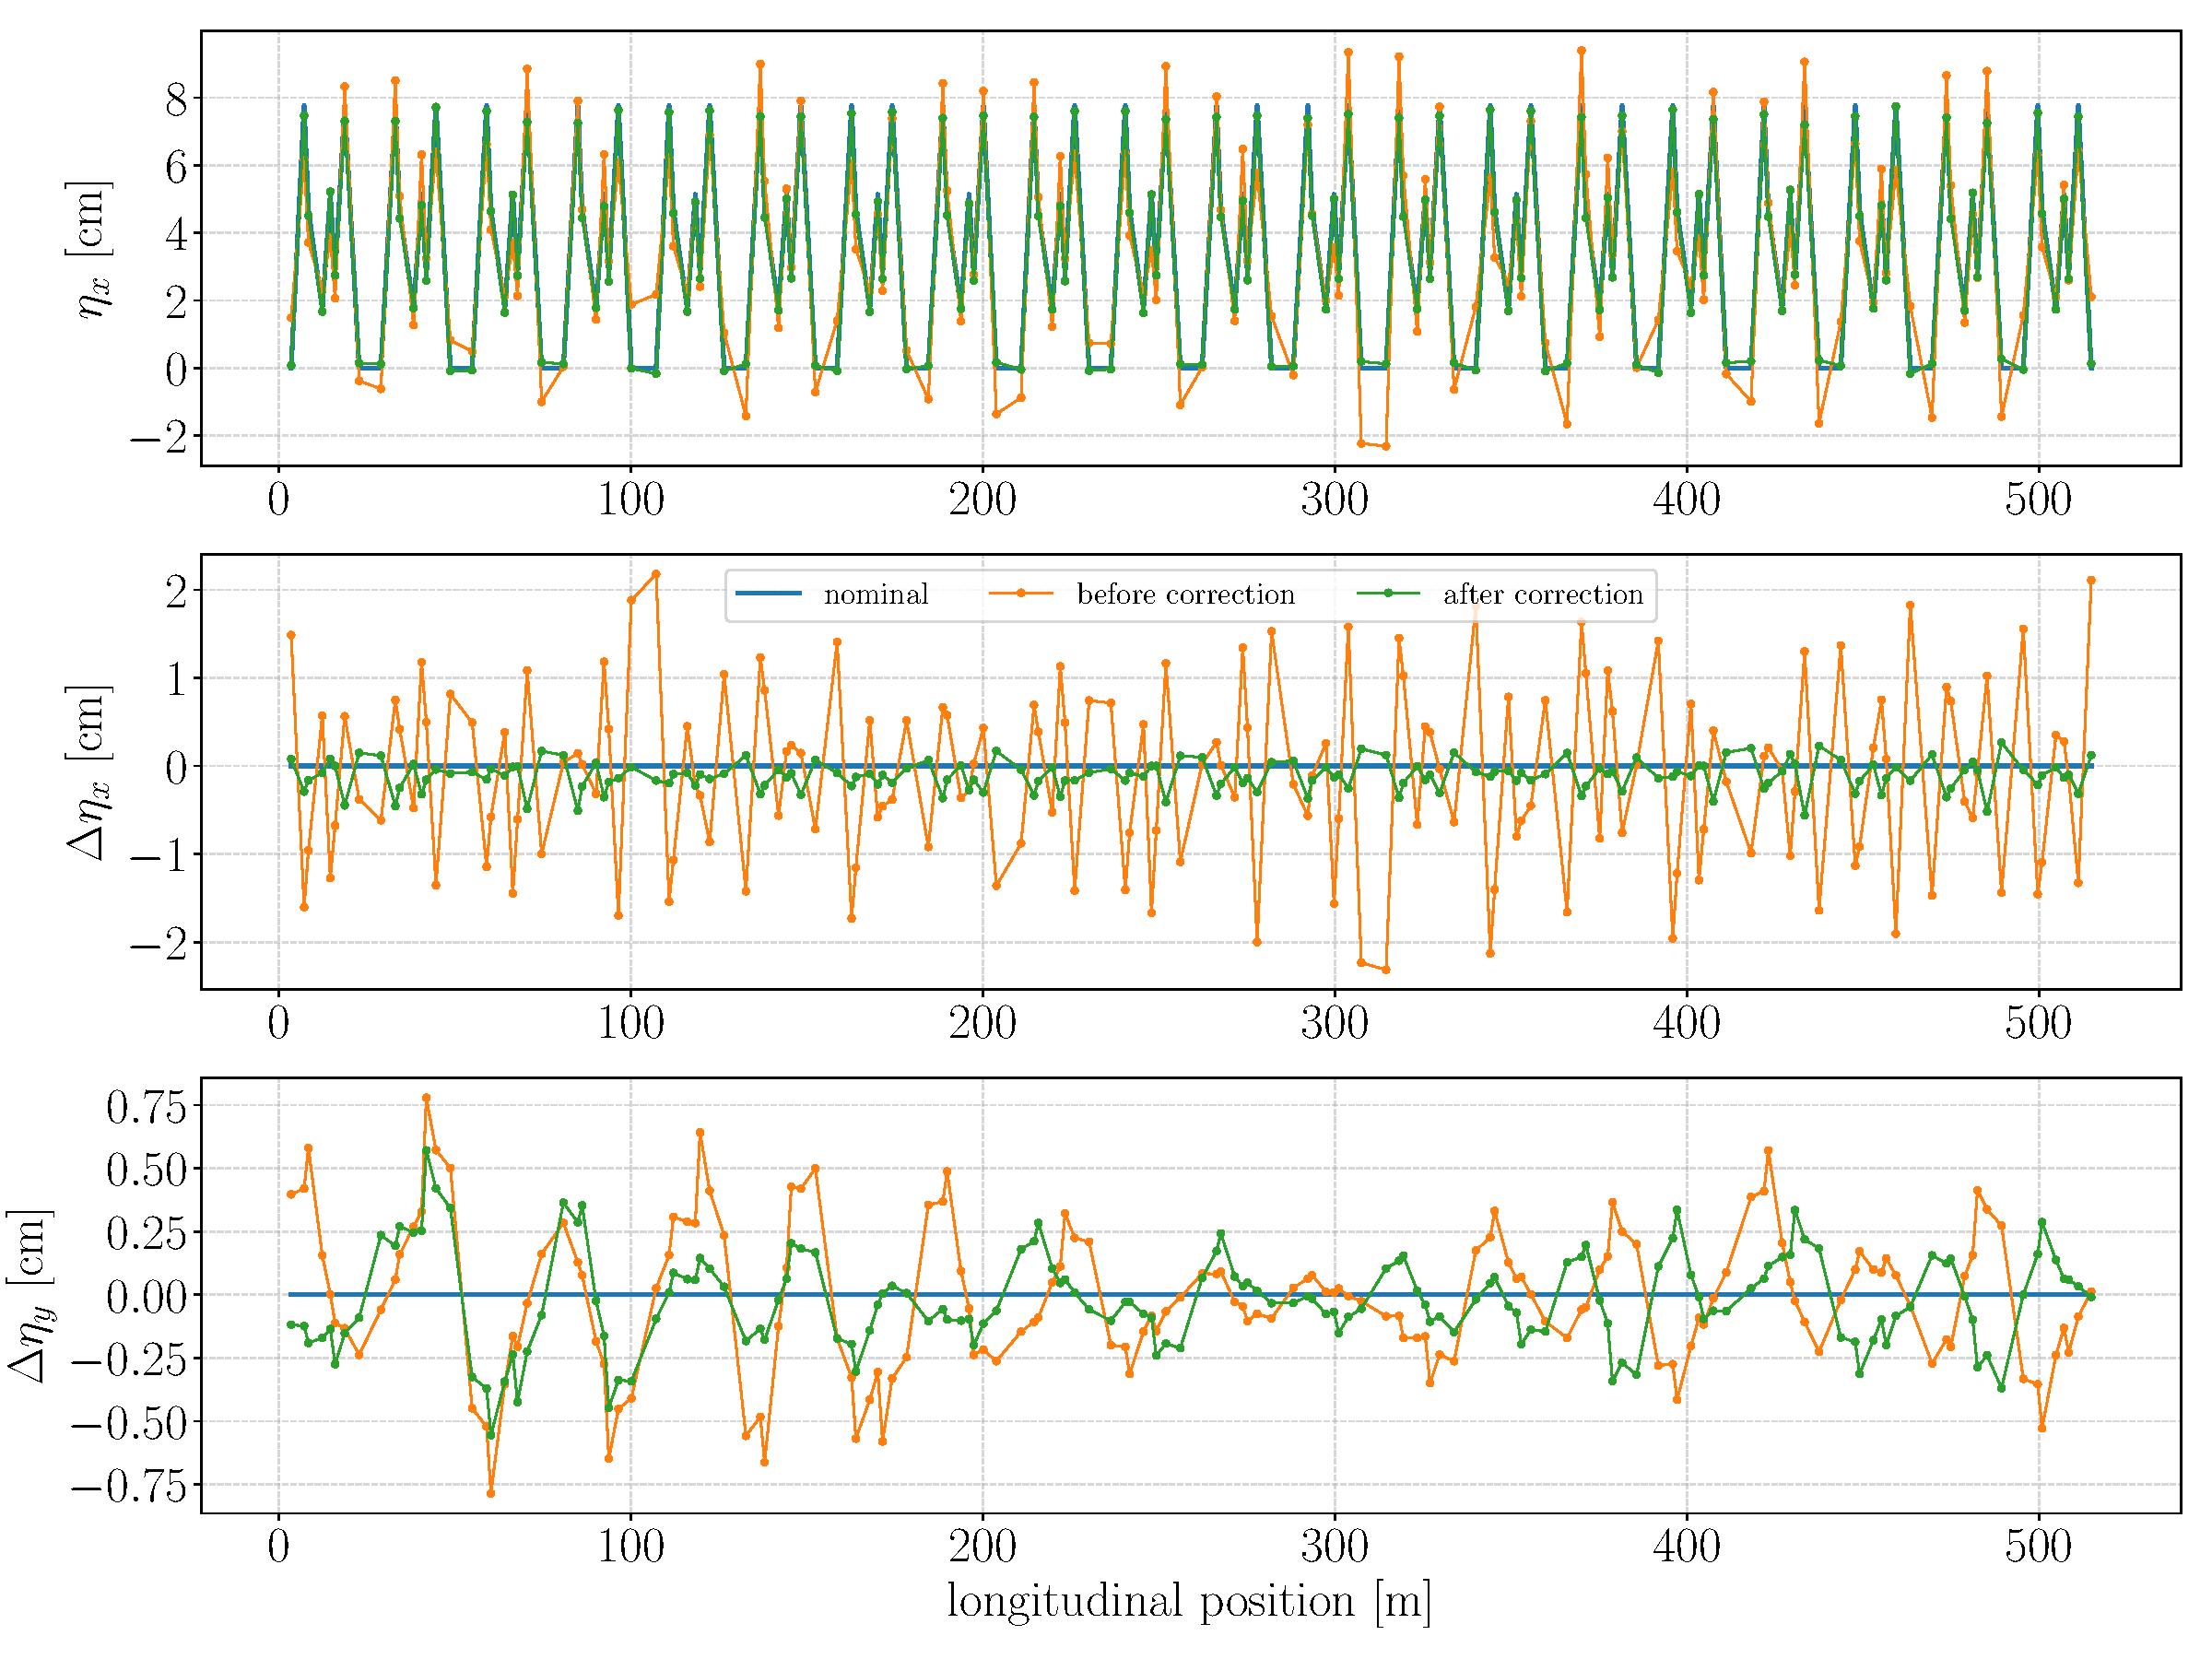
\includegraphics[width=1.0\textwidth]{figures/dispersion_after_before_loco_legend.pdf}
\caption{Measured dispersion functions on BPMs and its differences from nominal values.}
\label{fig:disp_error}
\end{figure}

It can be observed that the horizontal dispersion errors were greatly reduced, especially in straight sections, were $\eta_x = 0$ nominally. However, the errors in vertical dispersion could not be reduced with the same effectiveness. This was already expected, since the LOCO calibrated models predicted $\eta_y$ functions very different from the measured ones. Initially the std error for $\eta_x$ was $\SI{10.2}{\milli\meter}$ and after the corrections it was reduced to $\SI{1.6}{\milli\meter}$. For $\eta_y$, these errors were $\SI{2.8}{\milli\meter}$ before and $\SI{1.9}{\milli\meter}$ after LOCO. From Table~\ref{tab:calibrated_optics}, it is seen that LOCO model accurately predicted the values obtained in the actual storage ring for $\eta_x$. On the other hand, even though the initial predicted and measured  $\eta_y$ are in concordance, the final $\eta_y$ error calculated with the calibrated model is about 4 times lower than the corresponding measured error. This incompatibility will be further discussed in Section~\ref{sec:orbit_effect}.

\subsection{Betatron Function}
There is a quite simple method for measuring the betatron function. In Subsection~\ref{subsec:optics} it is discussed how gradient errors perturb the linear optics on a storage ring. In Appendix~\ref{appendix:beta} the effect of a single gradient error in a quadrupole of length $L$ on the betatron tunes, given the beta function, is calculated. The process can be reversed: intentionally changing the integrated gradient of a single quadrupole by a small amount $\Delta \mathrm{KL}$ and measuring the corresponding tune shift, the integral of beta function along the quadrupole is calculated as:
\begin{align}
\dfrac{1}{L}\int_{0}^{L} \beta_u(s) \mathrm{d}s &= 4\pi\frac{\Delta \nu_u}{\Delta \mathrm{KL}},
\end{align}
where $u=x, y$. This method has the disadvantage that the gradient variation $\Delta \mathrm{KL}$ applied in the quadrupole must be well known, otherwise this introduces systematic errors in beta calculation. Since the tune measurements are typically very precise, the contribution of the error of $\Delta \nu_u$ to the beta function measurement is negligible.

This process, which will be called beta measurement by individual quadrupole variation, can be performed for each quadrupole to measure the betatron functions around the storage ring. Then, the obtained values can be compared to the nominal ones, which is calculated numerically with the model, simulating the described process, or evaluated with analytical expressions, derived in Appendix~\ref{appendix:beta}.

The author implemented the beta measurement for Sirius storage ring in a Python script and the code can be accessed in its GitHub Repository~\cite{betasirius}. The script also performs the data analysis and evaluates the beta integrals for a given Sirius storage ring model, returning both measured and model beta integrals at quadrupoles for comparison.

The measurement process was tested and adjusted several times. After 10~\gls{orm}s were measured to obtain the fit parameters variations as discussed in Subsection~\ref{subsec:fit_var}, 10 sequential beta measurements were performed as well\footnote{Again, the repeatability test for optics function measurements was performed after LOCO corrections.}. Calculating the dispersion function from the 10 measured~\gls{orm}s, the variations for lattice functions measurements in Sirius storage ring were obtained and the results are organized in Table~\ref{tab:twiss_var_meas}.
% \begin{table}
%     \centering
%     \caption{Variations in lattice functions for 10 sequential measurements performed in Sirius storage ring.}
%     \label{tab:twiss_var_meas}
%     \begin{tabular}{cccc}
%         \toprule\toprule
%         Lattice function & std variation & peak-to-valley variation & Unit \\
%         \hline
%         $\beta_x$ & \num{0.8}& \num{4.3} & \%\\
%         $\beta_y$ & \num{0.5} & \num{4.2}& \% \\
%         $\eta_x$ & \num{0.2} & \num{0.9} & \SI{}{\milli\meter}\\
%         $\eta_y$ & \num{0.3} & \num{1.3} & \SI{}{\milli\meter} \\
%         \bottomrule\bottomrule
%     \end{tabular}
% \end{table}
\begin{table}
    \centering
    \caption{Variations in lattice functions for 10 sequential measurements performed in Sirius storage ring.}
    \label{tab:twiss_var_meas}
    \begin{tabular}{ccccc}
        \toprule\toprule
        Lattice function error & mean rms & rms variation & peak-to-valley rms & Unit \\
        \hline
        $\Delta \beta_x/\beta_x$ & \num{3.9}& \num{0.8}  & \num{4.3} & \%\\
        $\Delta \beta_y/\beta_y$ & \num{4.1} & \num{0.5} & \num{4.2} & \% \\
        $\Delta \eta_x$ & \num{1.6} & \num{0.2} &          \num{0.9} &   \SI{}{\milli\meter}\\
        $\Delta \eta_y$ & \num{1.9} & \num{0.3} &          \num{1.3} & \SI{}{\milli\meter} \\
        \bottomrule\bottomrule
    \end{tabular}
\end{table}

The~\gls{std} variations for each point were used to define the related error bars, which is this case are related to random errors. Note that dispersion function measurement variations are low, due to the fact that~\gls{rf} frequency changes are precise and well-known. On the other hand, variations in beta measurement are on the order of few percent. The main cause for this is hysteresis in the quadrupoles gradient fields. It is desirable to correct the storage ring linear optics in the level of the measurement's errors. From simulations with random errors in the model, it was possible to obtain beta-beatings~\gls{std} as low as $1\%$.

The implemented script was applied to obtain the Sirius beta functions before and after the application of LOCO corrections in quadrupole's trim-coils and the results are shown in Figure~\ref{fig:beta_tuneshift}. The corresponding beta-beatings for the measured values are plotted in Figure~\ref{fig:beta_beating_progress}.
\begin{figure}
\centering
\begin{subfigure}[t]{0.49\textwidth}
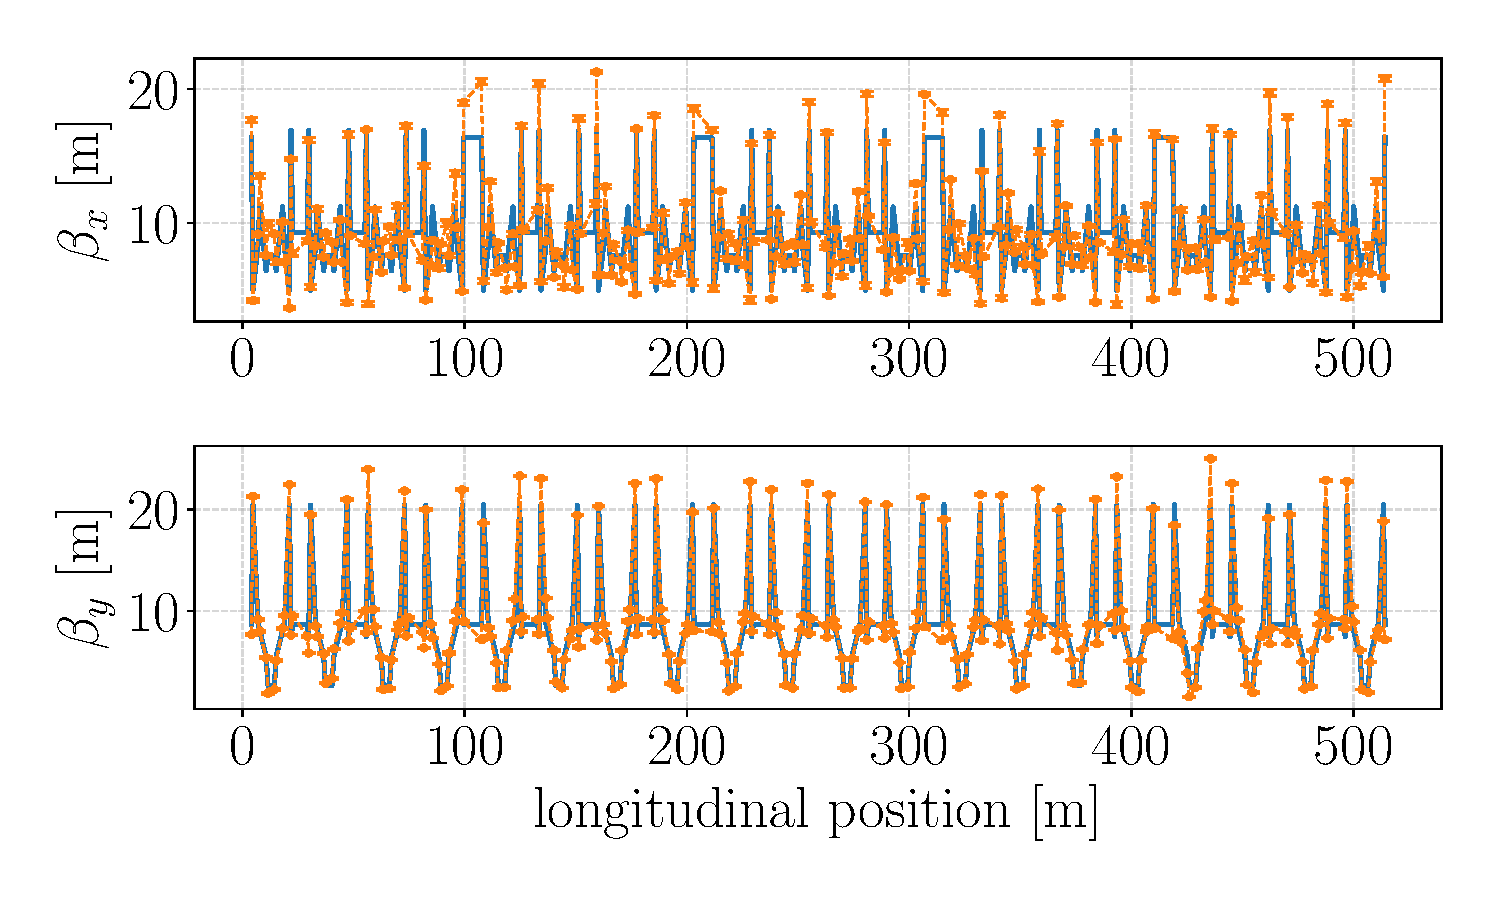
\includegraphics[width=1.0\textwidth]{figures/beta_before_big.pdf}
    \caption{Before.}
    \label{subfig:beta_before}
\end{subfigure}
 \begin{subfigure}[t]{0.49\textwidth}
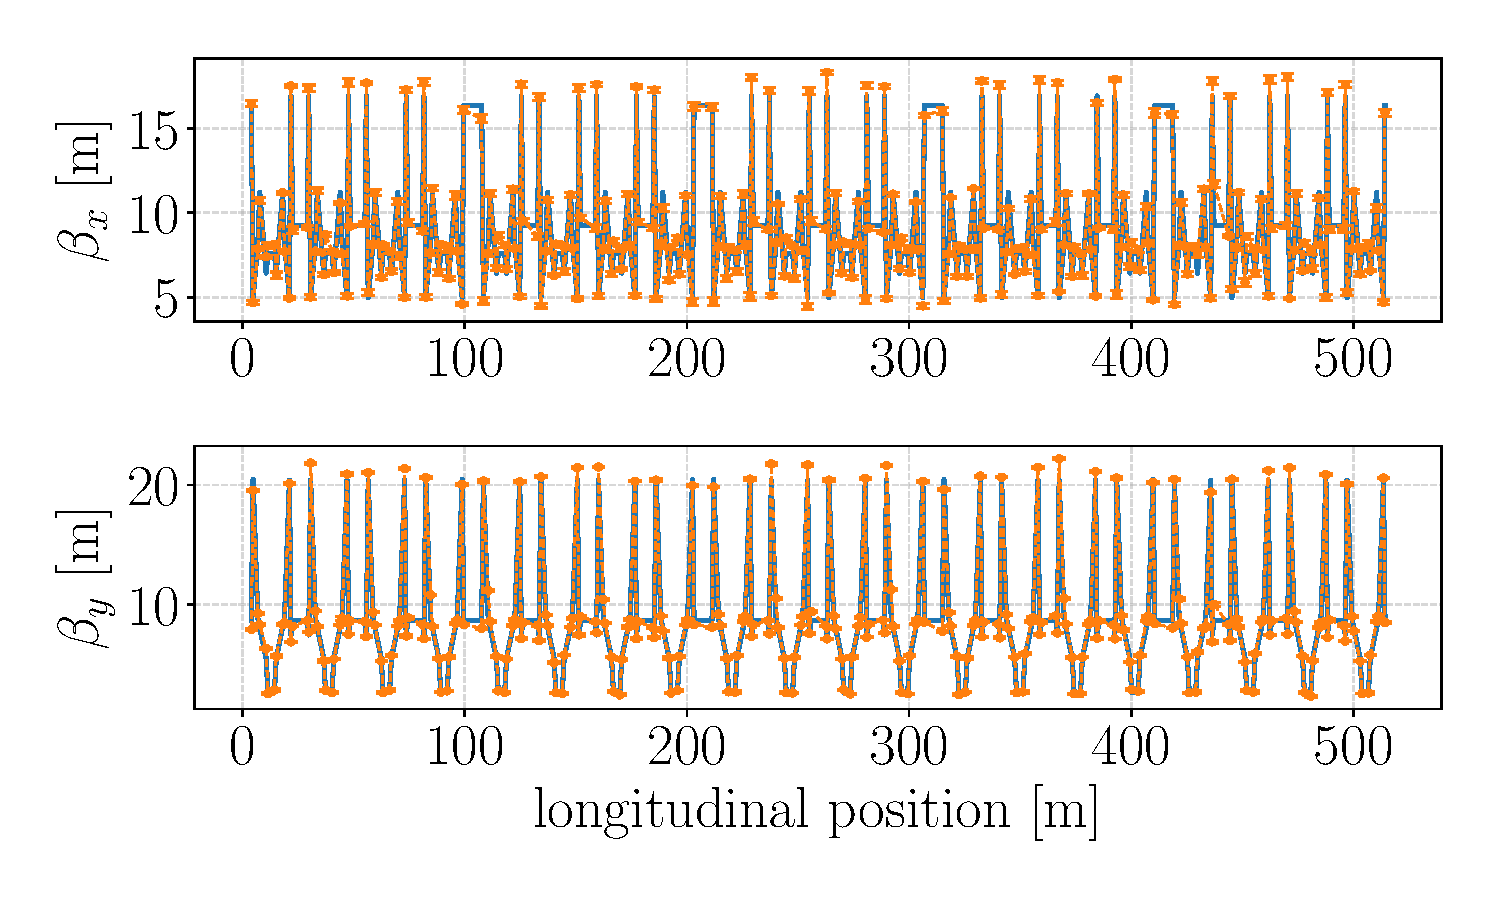
\includegraphics[width=1.0\textwidth]{figures/beta_after_big.pdf}
    \caption{After.}
    \label{subfig:beta_after}
\end{subfigure}
\caption{Nominal (blue) and measured (orange) betatron functions before and after LOCO corrections.}
\label{fig:beta_tuneshift}
\end{figure}
\begin{figure}
\centering
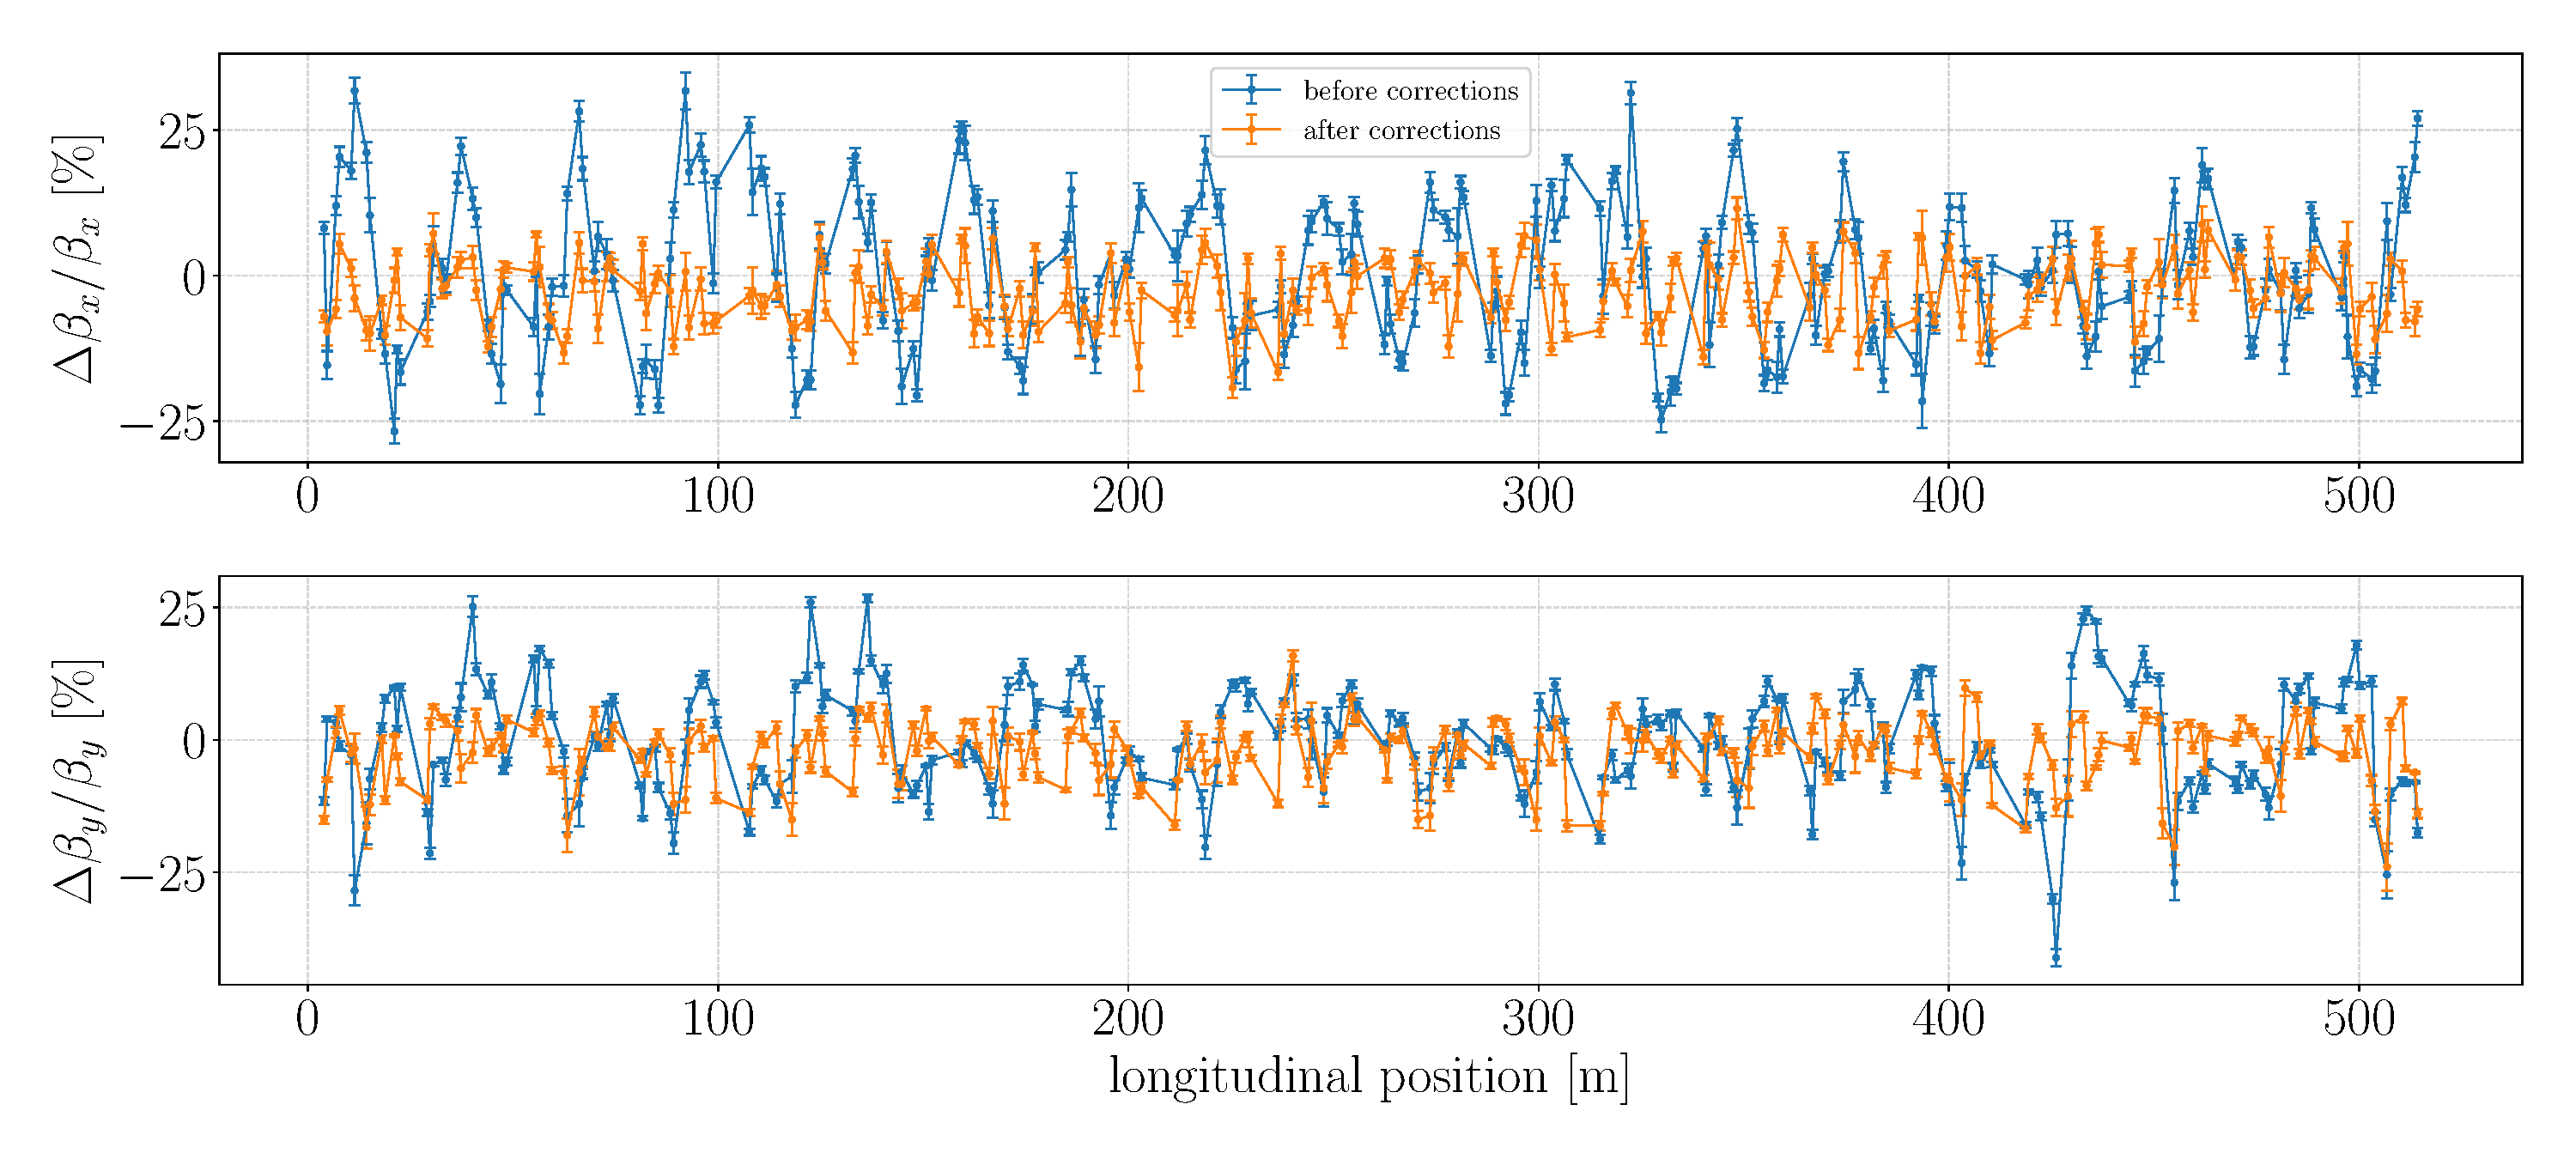
\includegraphics[width=1.0\textwidth]{figures/beta_beating_progress_big.pdf}
\caption{Comparsion of beta-beating before and after optics corrections.}
\label{fig:beta_beating_progress}
\end{figure}

Before LOCO corrections, measured horizontal and vertical beta-beatings (std) were $\SI{12.8(8)}{\%}$ and $\SI{10.4(5)}{\%}$, respectively. With new gradients settings these values were reduced to $\SI{3.9(8)}{\%}$ and $\SI{4.1(5)}{\%}$.

An alternative method to measure beta functions can be performed by applying~\gls{pca} in~\gls{tbt} position measurements from~\glspl{bpm}. The beam trajectory can be perturbed with a dipolar impulse, applied by an element in the storage ring called pinger, that excites betatron oscillations that can be acquired with~\glspl{bpm}. The oscillation harmonics encoded in the BPM data can be identified and separated with~\gls{pca}. The two main components for each plane of oscillation are related to the betatron motion and from these two main harmonics it is possible to extract the beta functions and the phase advances in BPMs. For more details about the method, the author recommends the reference~\cite{huang2019beam}.

In Sirius storage ring, the dipolar kicker, used for on-axis injection, can also be used as a horizontal pinger. When these measurements were conducted, a vertical pinger was not available, so it was possible to measure only the horizontal beta function in~\glspl{bpm} using~\gls{pca} method. These measurements were done before and after LOCO corrections, using a small kick of $\SI{100}{\micro\radian}$ and analysing the~\gls{tbt} data for 4000 turns. The horizontal beta-beatings obtained were compared with measurements by individual quadrupole variation and with the predicted beta-beating from LOCO calibrated models. These results are plotted in Figure~\ref{fig:betax_compare}.
\begin{figure}
\centering
\begin{subfigure}[t]{1.0\textwidth}
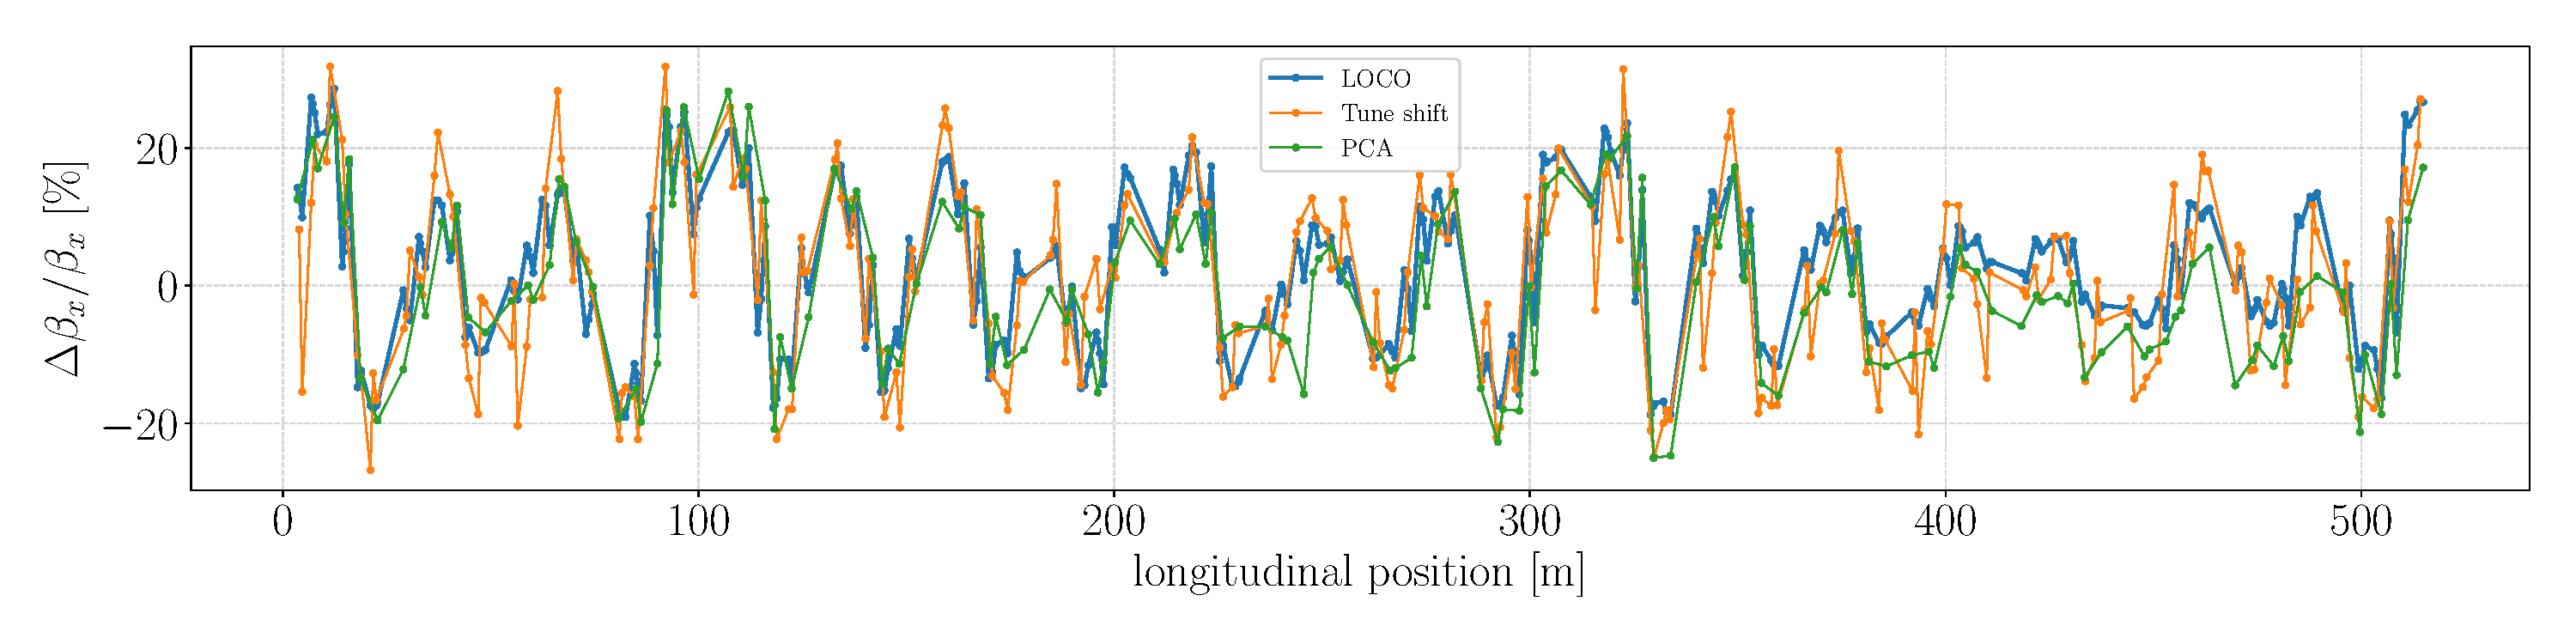
\includegraphics[width=1.0\textwidth]{figures/betax_compare_loco_pca_quad_before_corr.pdf}
    \caption{Before correction.}
    \label{subfig:betax_compare_before}
\end{subfigure}
 \begin{subfigure}[t]{1.0\textwidth}
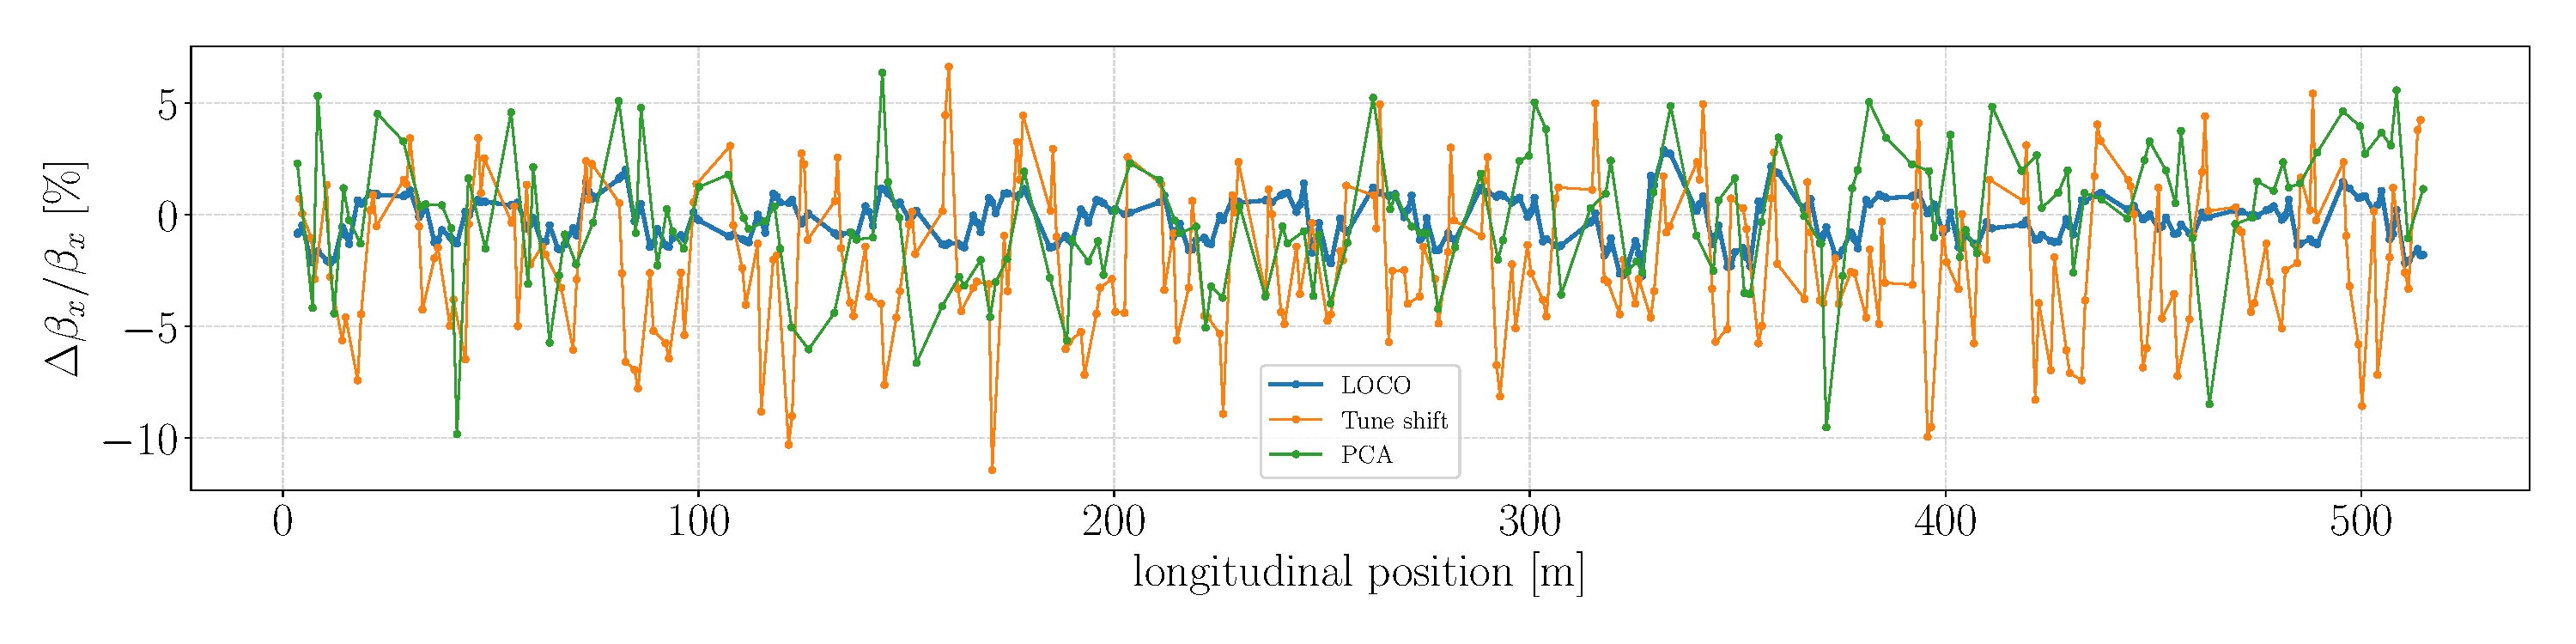
\includegraphics[width=1.0\textwidth]{figures/betax_compare_loco_pca_quad_after_corr.pdf}
    \caption{After correction.}
    \label{subfig:betax_compare_after}
\end{subfigure}
\caption{Horizontal beta-beating comparison between predicted beta with LOCO model and beta measurements: at quadrupoles based on tune shifts and at BPMs based on PCA applied on TbT data.}
\label{fig:betax_compare}
\end{figure}

Before LOCO corrections, the three measurements agreed quite well. The correlation between LOCO and PCA beta-beating signatures is $91\%$ and between LOCO and tune shifts is $86\%$. On the other hand, it can be seen that after the corrections, the LOCO model fails to predict the measured beta-beating in storage ring. In this situation, the correlation between LOCO and PCA values is $39\%$ and LOCO and tune shifts it is only $8\%$. The same is valid for~\gls{std} beta-beating, before corrections the values were; LOCO: $\SI{11.3}{\%}$, tune shift: $\SI{12.8}{\%}$, PCA: $\SI{11.5}{\%}$ and after corrections; LOCO: $\SI{1.0}{\%}$, tune shift: $\SI{3.3}{\%}$, PCA: $\SI{3.0}{\%}$. Then, in the latter case, the calibrated model predicted a horizontal beta-beating that is 3 times smaller than the measured values in Sirius storage ring. At this stage, this was an indication that the correspondence between the model and the actual ring was no longer valid. This will be further discussed in Section~\ref{sec:orbit_effect}.

% before: peak-to-valley x 58.6 y 67.9
% before: max abs x 31.8 y 41.1
% \\
% after: peak-to-valley x 36.9, y 38.8
% after  max abs x 26.4 y 26.8
\subsection{Betatron Coupling}
In Subection~\ref{subsec:linear_coupling} the effect of skew gradients on betatron coupling was briefly discussed. It was shown that a global parameter $|\kappa|$, called global betatron coupling, can be measured by approximating the betatron tunes, taking advantage on the fact that the tune difference resonance is stable. In the presence of coupling, the transverse tunes $\nu_x$ and $\nu_y$ are replaced by two normal tunes $\nu_1$ and $\nu_2$, also called eigentunes. This coupling problem can be formulated to be mathematically equivalent to the avoided-crossing problem in a two-level system in quantum mechanics. In this case, the matrix $\mathbf{C} = \begin{bmatrix} \nu_x & \kappa \\ \kappa & \nu_y \end{bmatrix}$ takes the place of the two-state hamiltonian and its eigenvalues are calculated as:
\begin{align}
    \nu_1 &= \dfrac{\nu_x + \nu_y}{2} + \dfrac{1}{2}\sqrt{\left(\dfrac{\nu_x - \nu_y}{2}\right)^2 + 4 \kappa^2}, \\
    \nu_2 &= \dfrac{\nu_x + \nu_y}{2} - \dfrac{1}{2}\sqrt{\left(\dfrac{\nu_x - \nu_y}{2}\right)^2 + 4 \kappa^2}.
    \label{eq:normal_tunes}
\end{align}

The equations above are equivalent to Eq.~\eqref{eq:eigentunes}. In the limit $\nu_x = \nu_y$, we also obtain that $\nu_1 - \nu_2 = |\kappa|$.

The tunes approximation can be performed by changing the focusing strengths in the storage ring. In Sirius, the fractional horizontal tune is lower than the vertical tune, thus the tunes can be approximated by increasing a focusing quadrupole strength. The QFB family was chosen for this experiment. If the current that feeds this quadrupole family is changed by $\Delta I_{\mathrm{QFB}}>0$, there is a corresponding change in horizontal tune $\Delta\nu_x > 0$ and vertical tunes $\Delta\nu_y < 0$. In this way, the tune sum and the difference can be viewed as functions of QFB current.

The measurement script and analysis was implemented by the~\gls{fac} and used by the author in Sirius storage ring to obtain the global betatron tunes before and after LOCO corrections. The results are shown in Figure~\ref{fig:global_coupling}. The gray curve presented in Figure~\ref{fig:global_coupling} was obtained by plugging the measured $\nu_x$, $\nu_y$ for each current $I_{\mathrm{QFB}}$ in matrix $\mathbf{C}$, diagonalizing it and fitting the parameter $\kappa$ and the offsets $(\nu_x+\nu_y)/2$ that minimize the quadratic difference to the data.
\begin{figure}
\centering
\begin{subfigure}[t]{0.49\textwidth}
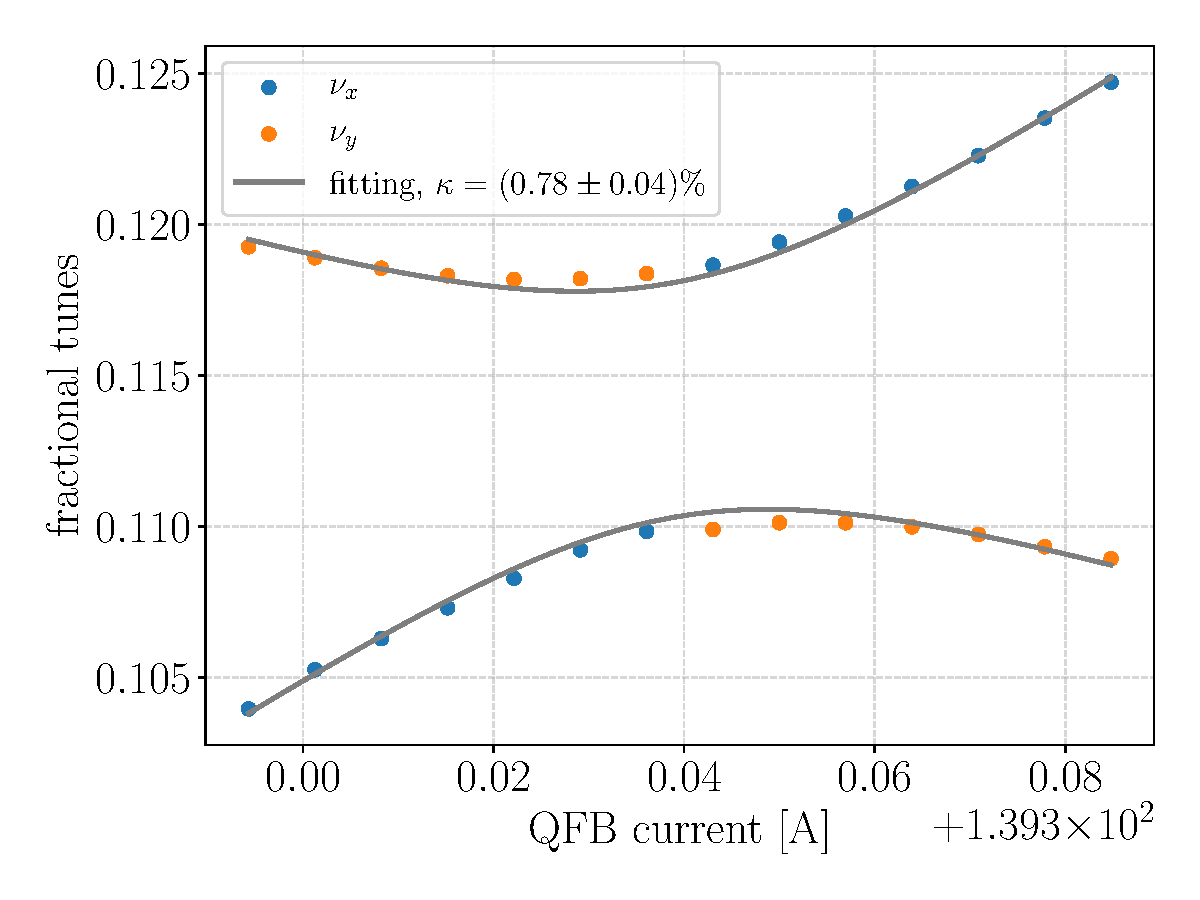
\includegraphics[width=1.0\textwidth]{figures/coupling_before_loco_grid_filter.pdf}
    \caption{Before.}
    \label{subfig:coup_before}
\end{subfigure}
 \begin{subfigure}[t]{0.49\textwidth}
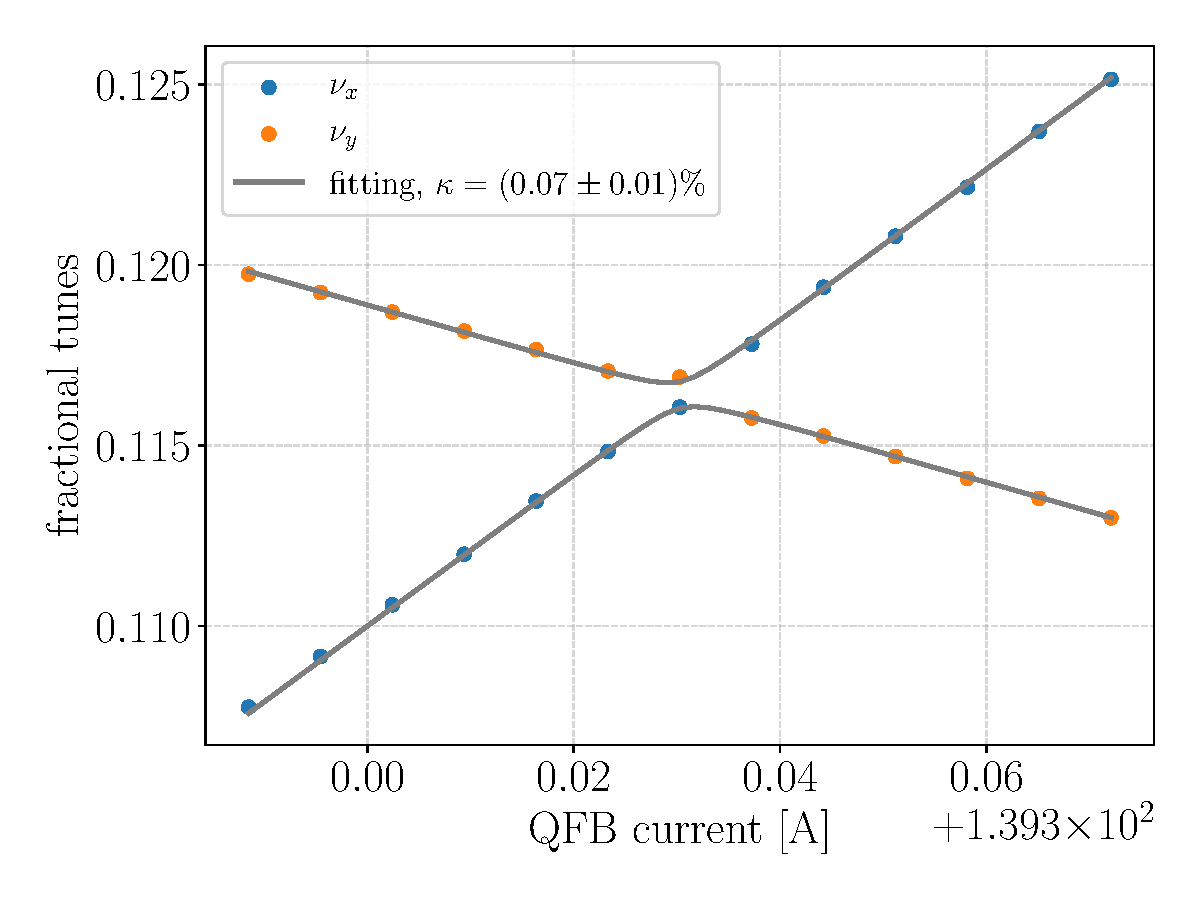
\includegraphics[width=1.0\textwidth]{figures/coupling_after_loco_grid_filter.pdf}
    \caption{After.}
    \label{subfig:coup_after}
\end{subfigure}
\caption{Global betatron coupling before and after LOCO corrections.}
\label{fig:global_coupling}
\end{figure}

For LOCO coupling corrections applied on skew quadrupoles, the residues used for minimization were $M_{xy}$ and $M_{yx}$, the~\gls{orm} off-diagonal elements, which are related to the local coupling along storage ring. However, the minimum tune difference measurements showed that the global betatron coupling was reduced as well, from the initial value of $\SI{0.78(4)}{\%}$ to $\SI{0.07(1)}{\%}$.

It is important to mention the goal coupling for Sirius storage ring is not necessarily small. The coupling parameter is somewhat a free parameter that can be varied to suit other purposes, for example to increase the beam lifetime or the vertical beam size. Neverthless, a common procedure is to first reduce the betatron coupling as much as possible, then increase the coupling towards the goal value in a controlled manner. With these studies, it was proved that LOCO is a robust method to minimize the off-diagonal~\gls{orm} elements and in this process the global betatron coupling is consequently reduced. However, even though the measured betatron coupling is near zero, since the vertical dispersion function could not be reduced with LOCO corrections, it is likely that the vertical beam emittance is still about $1\%$ of the horizontal emittance, as calculated with the first LOCO calibrated model.

\subsection{Horizontal Dynamic Aperture}
The horizontal pinger can also be used to apply dipolar impulses in the stored electron beam with increasing amplitudes until the beam is partially or totally lost. Measuring with BPMs the transverse oscillations over the turns, one can obtain how much beam is lost as a function of the transverse positions. This is basically the dynamic aperture measurement. Since only the horizontal pinger was available in Sirius storage ring, only the horizontal dynamic aperture could be measured.

Figure~\ref{fig:xdynap} shows the measurement results before and after optics and coupling corrections. Setting $5\%$ as the beam loss limit to estimate the dynamic aperture, after the application of LOCO corrections on linear optics and coupling, the horizontal dynamic aperture was increased from $\SI{7.6}{\milli\meter}$ to $\SI{8.3}{\milli\meter}$, which is an improvement of approximately $10\%$.
\begin{figure}
\centering
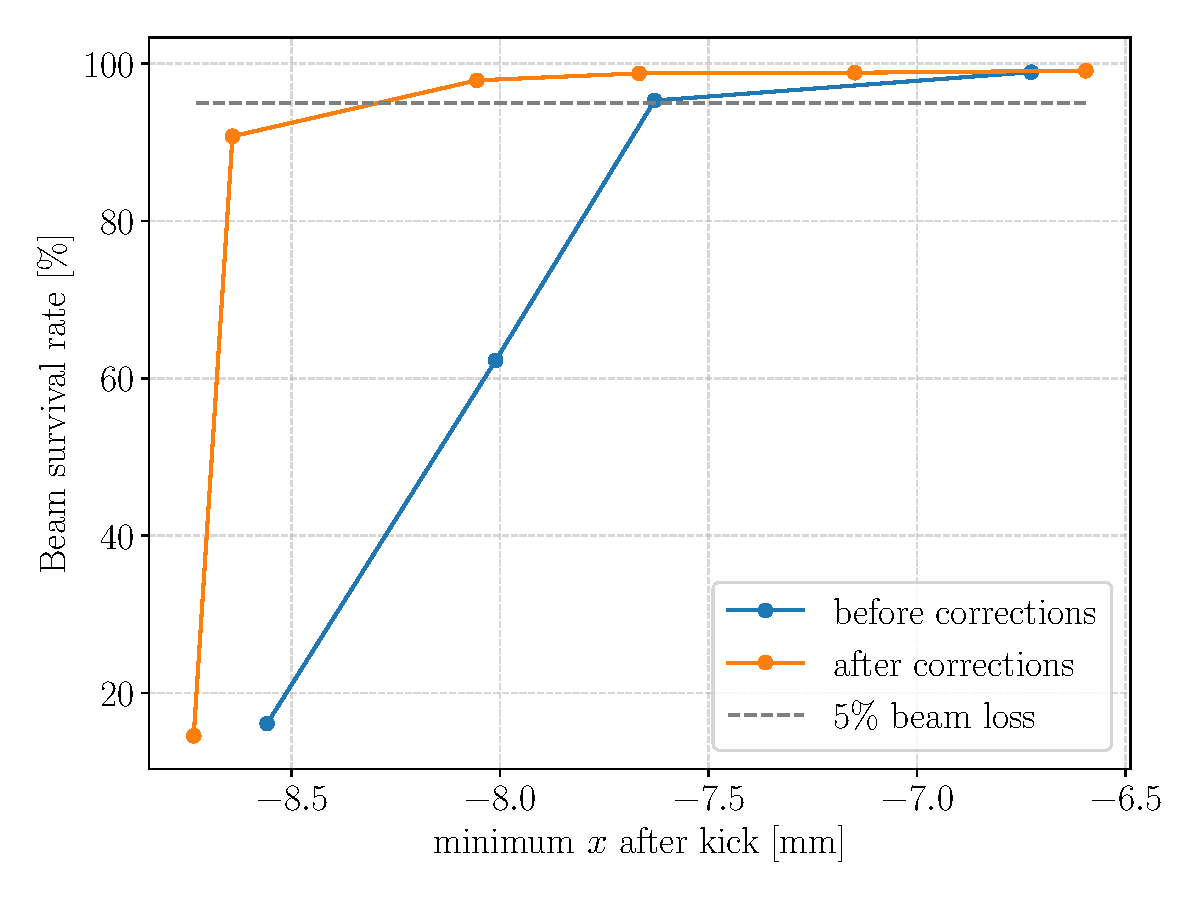
\includegraphics[width=0.75\textwidth]{figures/xdynamic_aperture_grid.pdf}
\caption{Comparison of horizontal dynamic aperture measurement before and after LOCO corrections.}
\label{fig:xdynap}
\end{figure}

The horizontal dynamic aperture is important for Sirius injection, given that a~\gls{nlk} is used to perform the off-axis injection in the storage ring. The off-axis injection occurs at $x=\SI{-8}{mm}$ from the vacuum chamber center, because at that location the~\gls{nlk} field is maximum. The~\gls{nlk} field rapidly decays as the position approaches $x=0$, causing no effect on the stored beam. More information about off-axis injection with~\gls{nlk} can be found in~\cite{liu2016a, wikinlk}.

To efficiently inject electrons from Booster with~\gls{nlk}, the storage ring dynamics at $x=\SI{-8}{mm}$ must be stable. From the simulations with Sirius storage ring model, including alignment and field errors (satisfying the specifications), the dynamic aperture obtained was $x=\SI{-9.5}{mm}$. Therefore, even with the improvement obtained with LOCO corrections, the measured horizontal dynamic aperture is still about $15\%$ lower than expected from simulations. 

It is worth to mention that beam dynamics in Sirius storage ring depends strongly of non-linear effects, which is well-known for~\glspl{4gsr}. At the time of writing, non-linear optimizations were not carried out in Sirius yet. This kind of optimization is one example of accelerator physics studies that might improve the storage ring dynamic aperture towards design values.

\subsection{Injection Efficiency}
To close this section of independent measurements, the injection efficiency in the storage ring was recorded before and after linear optics and coupling corrections. The data is presented in Figure~\ref{fig:injeff}. A linear fitting was applied on the data. The angular coefficient increased from $\SI{196}{\micro\ampere\second^{-1}}$ to $\SI{677}{\micro\ampere\second^{-1}}$. The Sirius injection rate is $\SI{2}{\hertz}$ and the current delivered by booster to the storage ring is $\SI{500}{\micro\ampere}$ on average, i.e, with an injection without any losses, the accumulation rate would be approximately $\SI{1}{\milli\ampere\second^{-1}}$. Therefore, with optics and coupling corrections, the average injection efficiency was increased from $20\%$ to $68\%$, which is an improvement of a factor $3.4$.
\begin{figure}
\centering
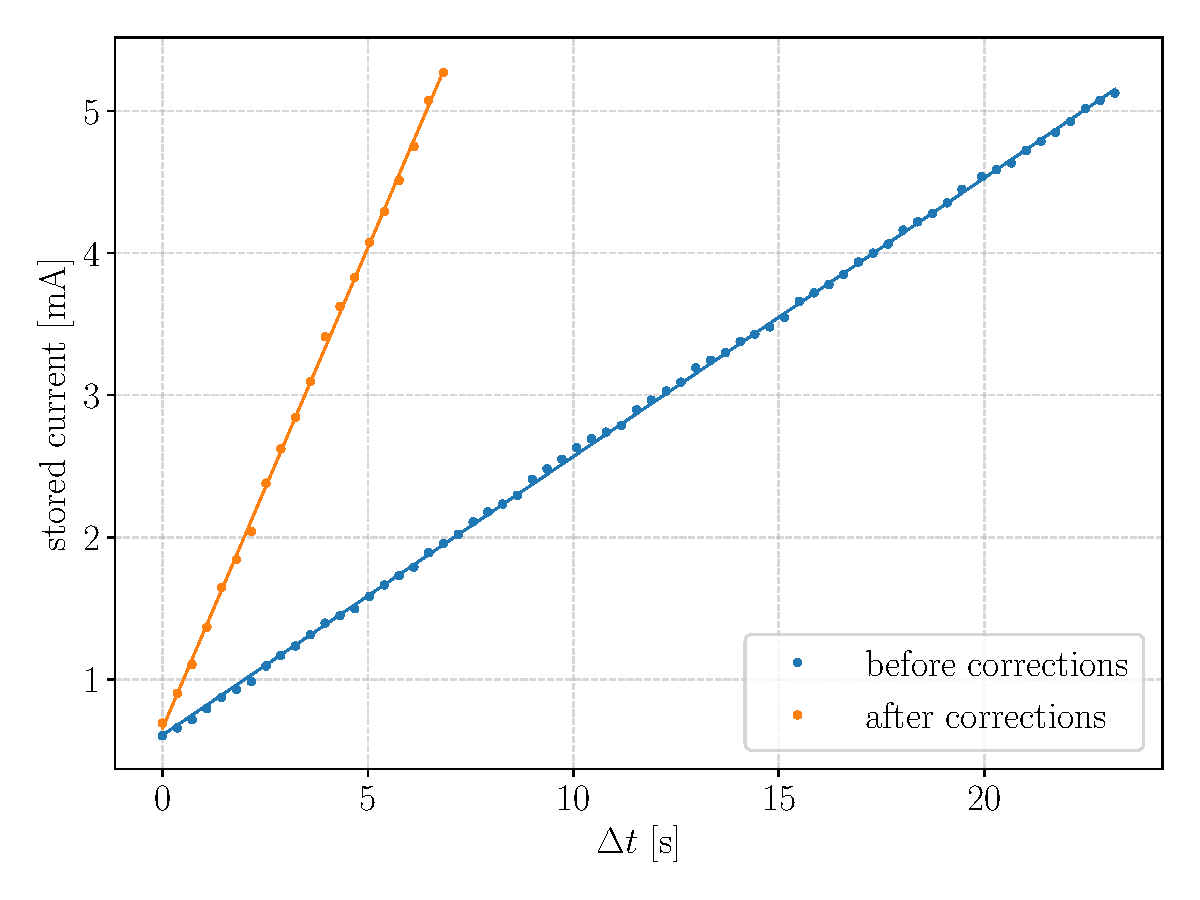
\includegraphics[width=0.75\textwidth]{figures/injeff_grid.pdf}
\caption{Beam accumulation before and after LOCO corrections.}
\label{fig:injeff}
\end{figure}
During the commissioning, large pulse-by-pulse variations on injection efficiency have been observed. The changes in injection efficiency recorded were as high as $20\%$. This problem might be related to the dynamic aperture, since its measured value indicates that the electron beam had to be injected in the dynamic aperture edge in order to receive the required kick from~\gls{nlk}. In this situation, any change of a few percent in the injection condition leads to electron losses. Leak fields from the injection pulsed magnets were also measured with the stored beam during the commissioning and shielding schemes are being studied to minimize their negative effects on injection. For the top-up injection mode on Sirius, an injection efficiency higher than $95\%$ with small pulse-by-pulse variation is required, so Sirius injection efficiency optimization was a work in progress at the time of writing. 

\section{Orbit Effect on Optics and Coupling}\label{sec:orbit_effect}
Orbit correction on Sirius storage ring was performed as follows: the BPM offsets with respect to quadrupoles centers were measured to define the~\gls{bba} orbit, then this orbit was used as the target for orbit correction. In this process, it was not possible to use all 281 singular values available in~\gls{orm} in the corrections, otherwise the correctors strengths would surpass the kick limits: $\pm \SI{330}{\micro\radian}$. Thus, it was necessary to use only 180 singular values in orbit correction and the final residual orbit, represented in Figure~\ref{fig:orbit_residue}, was obtained.
\begin{figure}
\centering
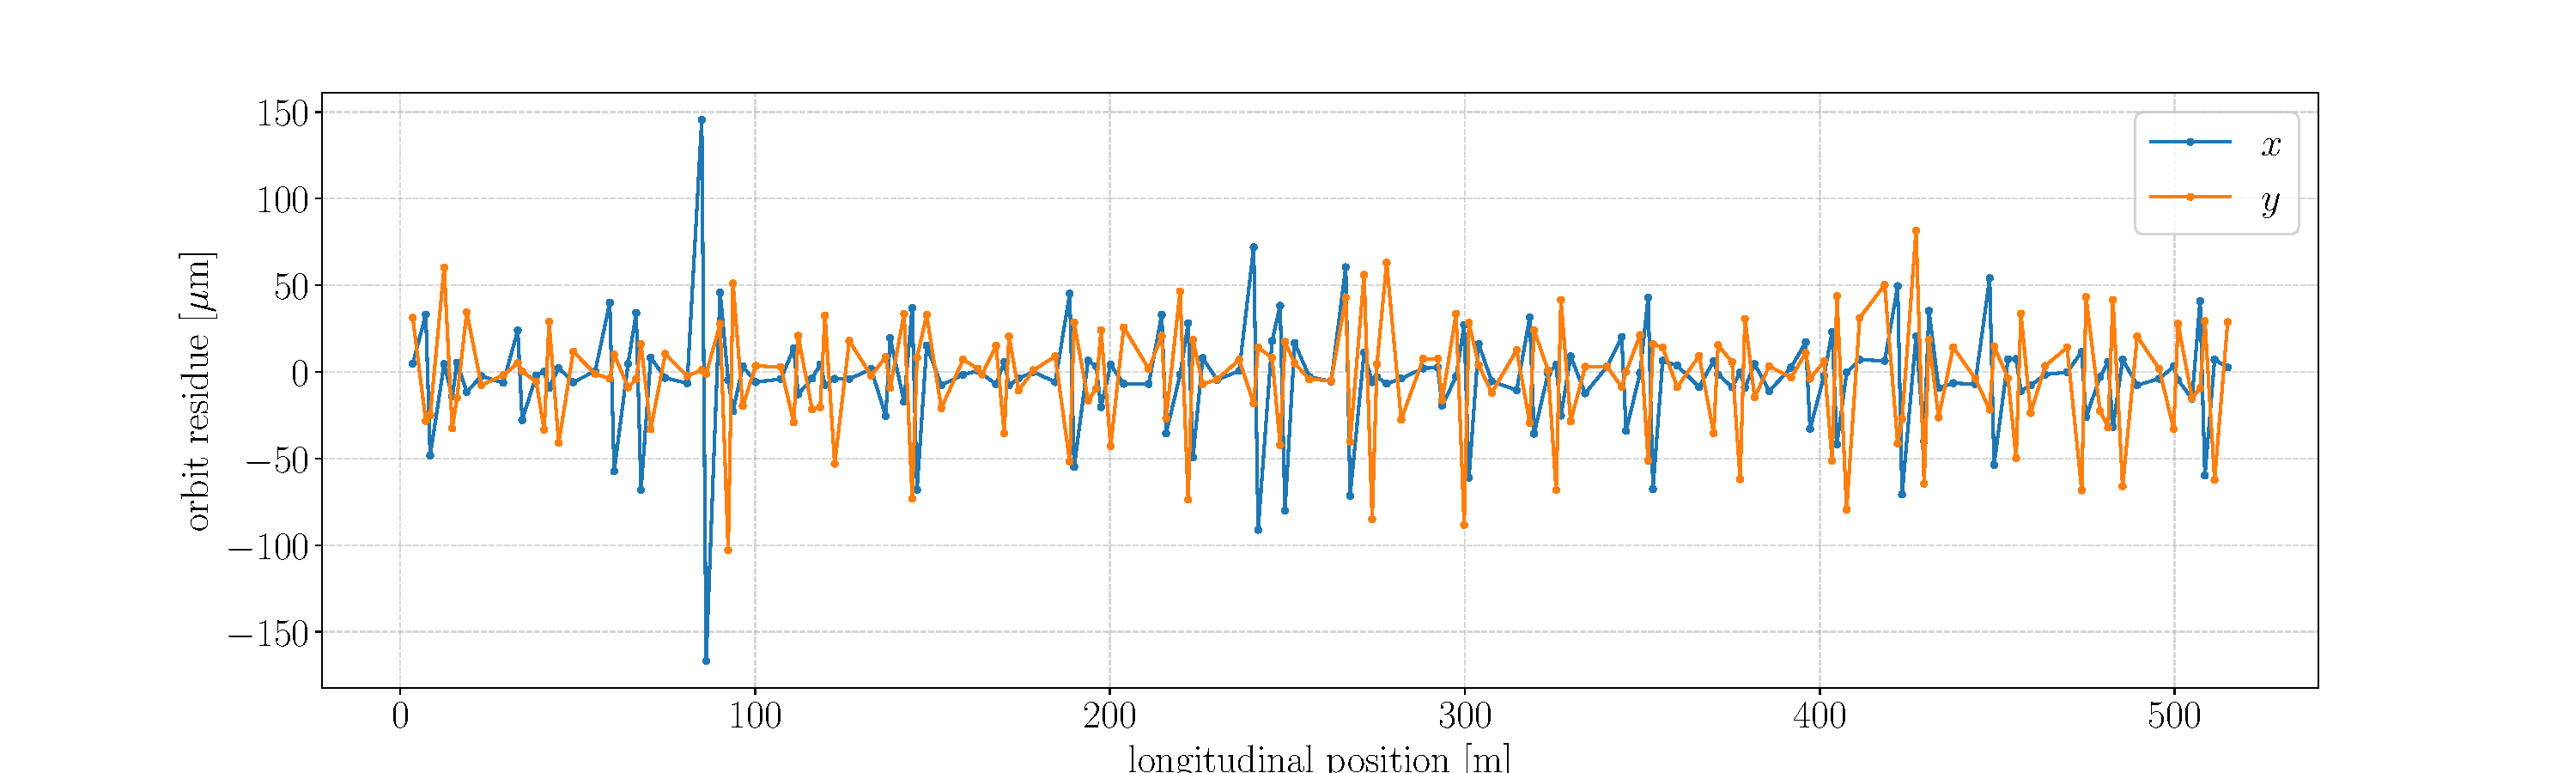
\includegraphics[width=1.0\textwidth]{figures/orbit_residue.pdf}
\caption{Residual orbit in Sirius storage ring.}
\label{fig:orbit_residue}
\end{figure}

The std values for the distortions in Figure~\ref{fig:orbit_residue} are $\SI{31}{\micro\meter}$ in horizontal plane and $\SI{32}{\micro\meter}$ in vertical. The peak-to-valley values are $\SI{312}{\micro\meter}$ and $\SI{184}{\micro\meter}$ for $x$ and $y$, respectively. From simulations, with alignment and field errors (within specified tolerances) on storage ring model, the orbit correction performance was better than the obtained in the actual ring, with std of $\SI{17}{\micro\meter}$ in the horizontal plane and nanometric std orbit vertically. This is an indicative that the real alignment errors are greater than the specifications.

It is well-known that the magnetic fields in a storage ring depend on the relative transverse position of the beam with respect to the magnets centers. This is the feed-down effect that was already mentioned throughout this work and it is discussed in Appendix~\ref{appendix:feed-down}. Since very strong quadrupoles and sextupoles are used in Sirius~\gls{mba} lattice, it is expected that the dependencies of linear optics and coupling related to orbit distortions might play an important role.

To study the contribution of orbit distortion on optics and coupling, the residual orbit in the storage ring was reproduced in the nominal model. At this stage, the betatron tunes were $\nu_x = 48.917$ and $\nu_y = 13.961$, and the tunes were corrected to the nominal values. Note that the distorted orbit produced large tune shifts of $\Delta \nu_x = -0.18$ and $\Delta \nu_y = -0.19$. An~\gls{orm} was calculated with this model and was used as input for a LOCO fitting with the same configuration used for the fitting of measured~\gls{orm}s. The initial difference between this~\gls{orm} and the nominal was $\chi = \SI{8.7}{\micro\meter}$. After the fitting, the final difference was $\chi = \SI{0.7}{\micro\meter}$. Considering the measured Sirius BPM accuracy of $\SI{0.25}{\micro\meter}$ approximately, a rough estimate of this noise effect on data would increase the final $\chi$, being closer to the same level obtained in LOCO fittings from measured~\gls{orm} in the storage ring (about $\SI{0.95}{\micro\meter}$).

The qualitative behavior of LOCO fitting in this test was very similar to the fittings performed with the measured~\gls{orm}. The fitted~\gls{orm} was adjusted in a very good level, both in diagonal and off-diagonal blocks. It was necessary to include the dispersion function in the fitting with weight $2$, otherwise the horizontal dispersion obtained with the calibrated model would not match the dispersion from the perturbed orbit model. The vertical dispersion function could not be reproduced with LOCO model as well. 

Although there was no errors in BPM gains and roll angles and correctors gains, during the fitting these parameters were changed to adjust the~\gls{orm}. The results for these fit parameters are shown in Figure~\ref{fig:gain_fit_orb}.
\begin{figure}
\centering
\begin{subfigure}[t]{0.49\textwidth}
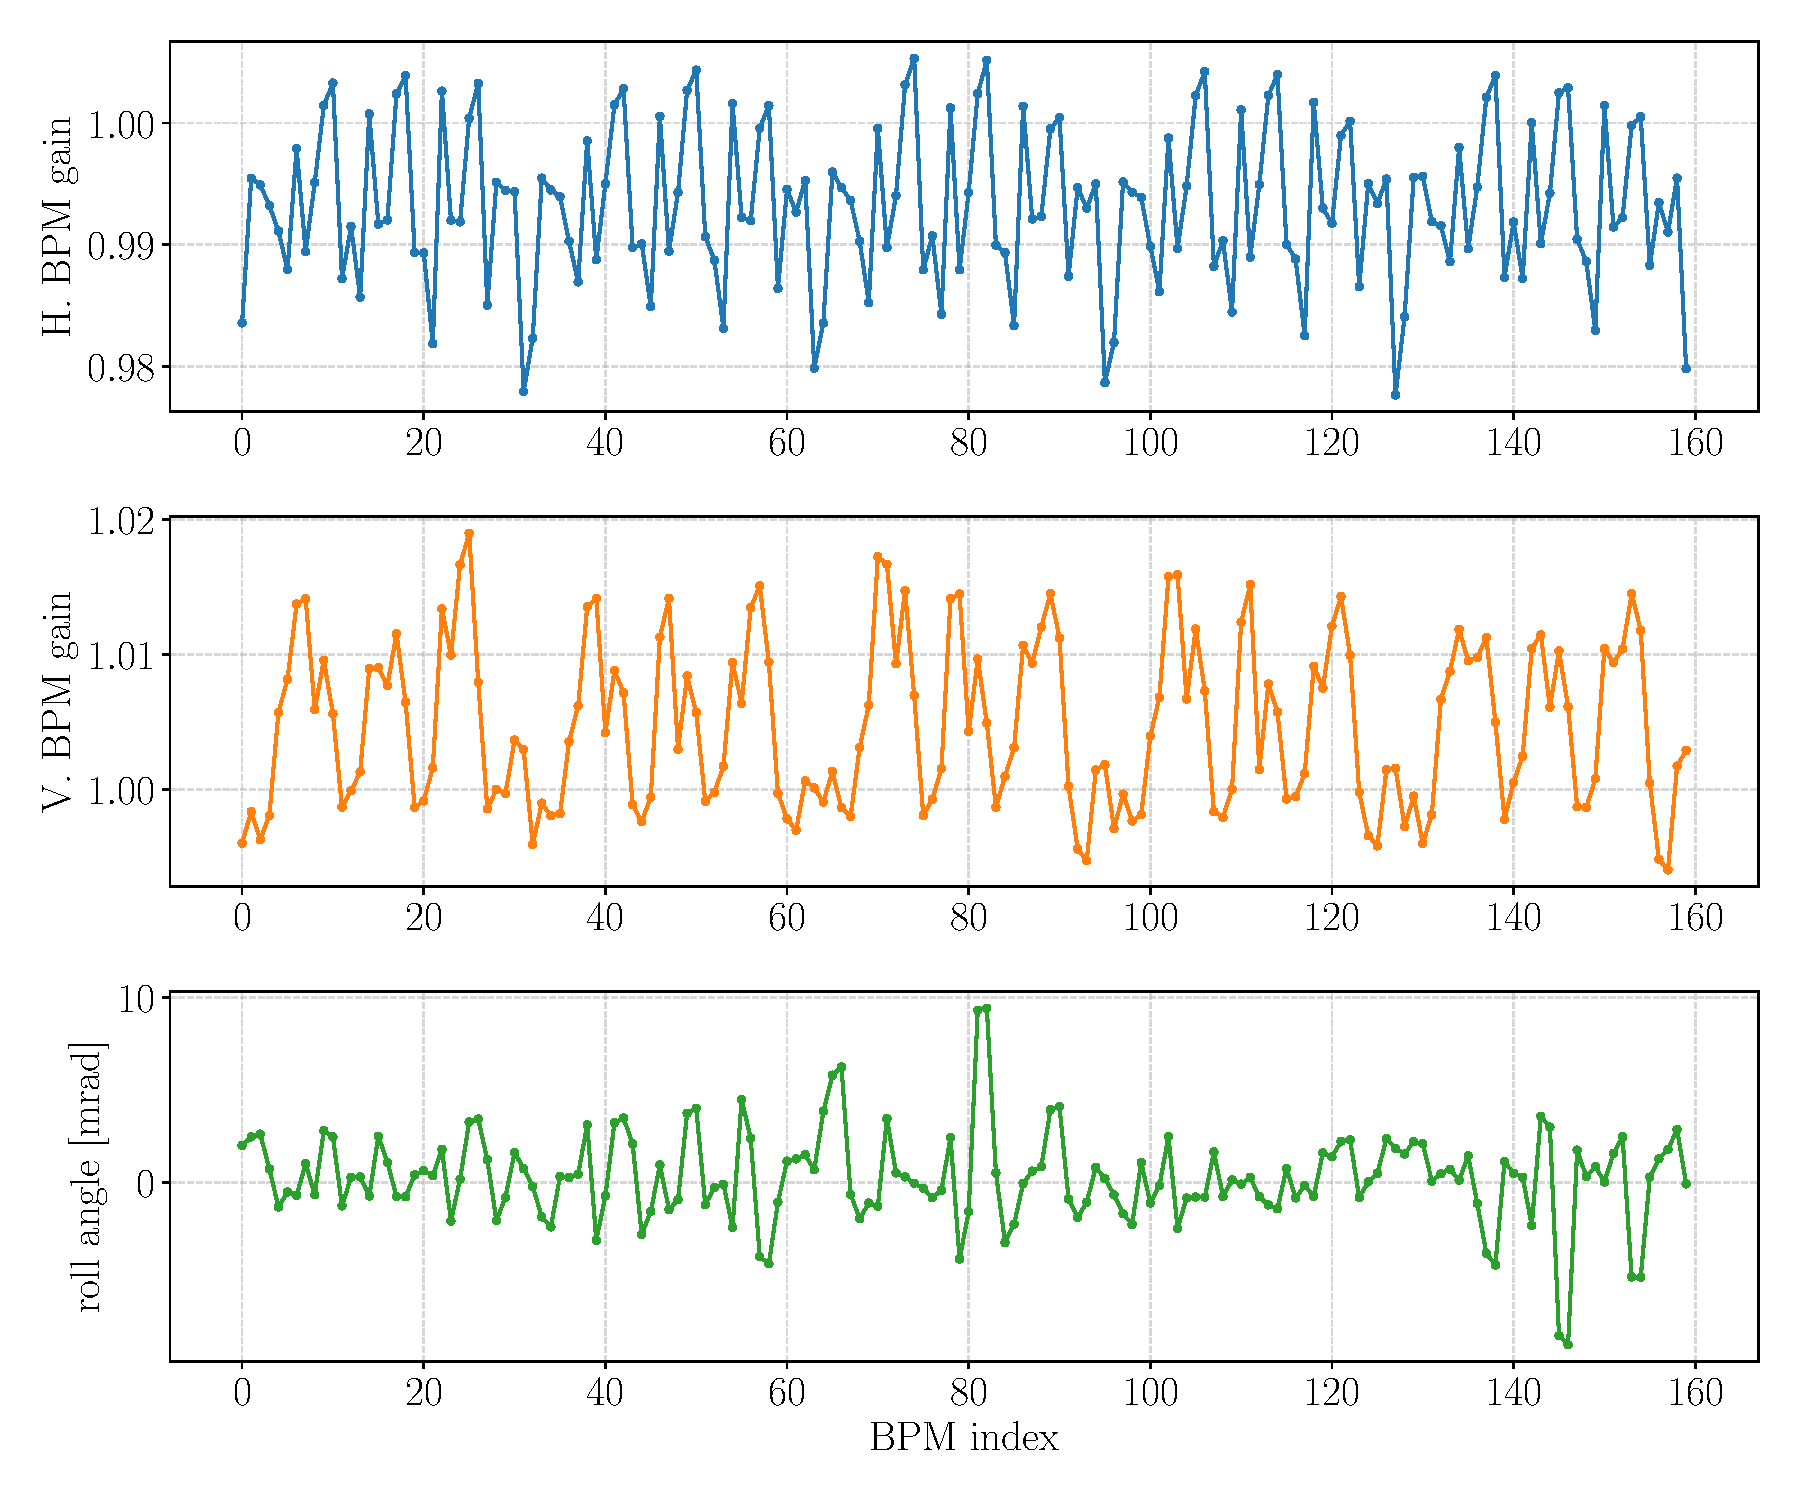
\includegraphics[width=1.0\textwidth]{figures/bpm_gains_orbit_distortion.pdf}
    \caption{BPM gains and roll angles.}
    \label{subfig:bpm_fit_orb}
\end{subfigure}
 \begin{subfigure}[t]{0.49\textwidth}
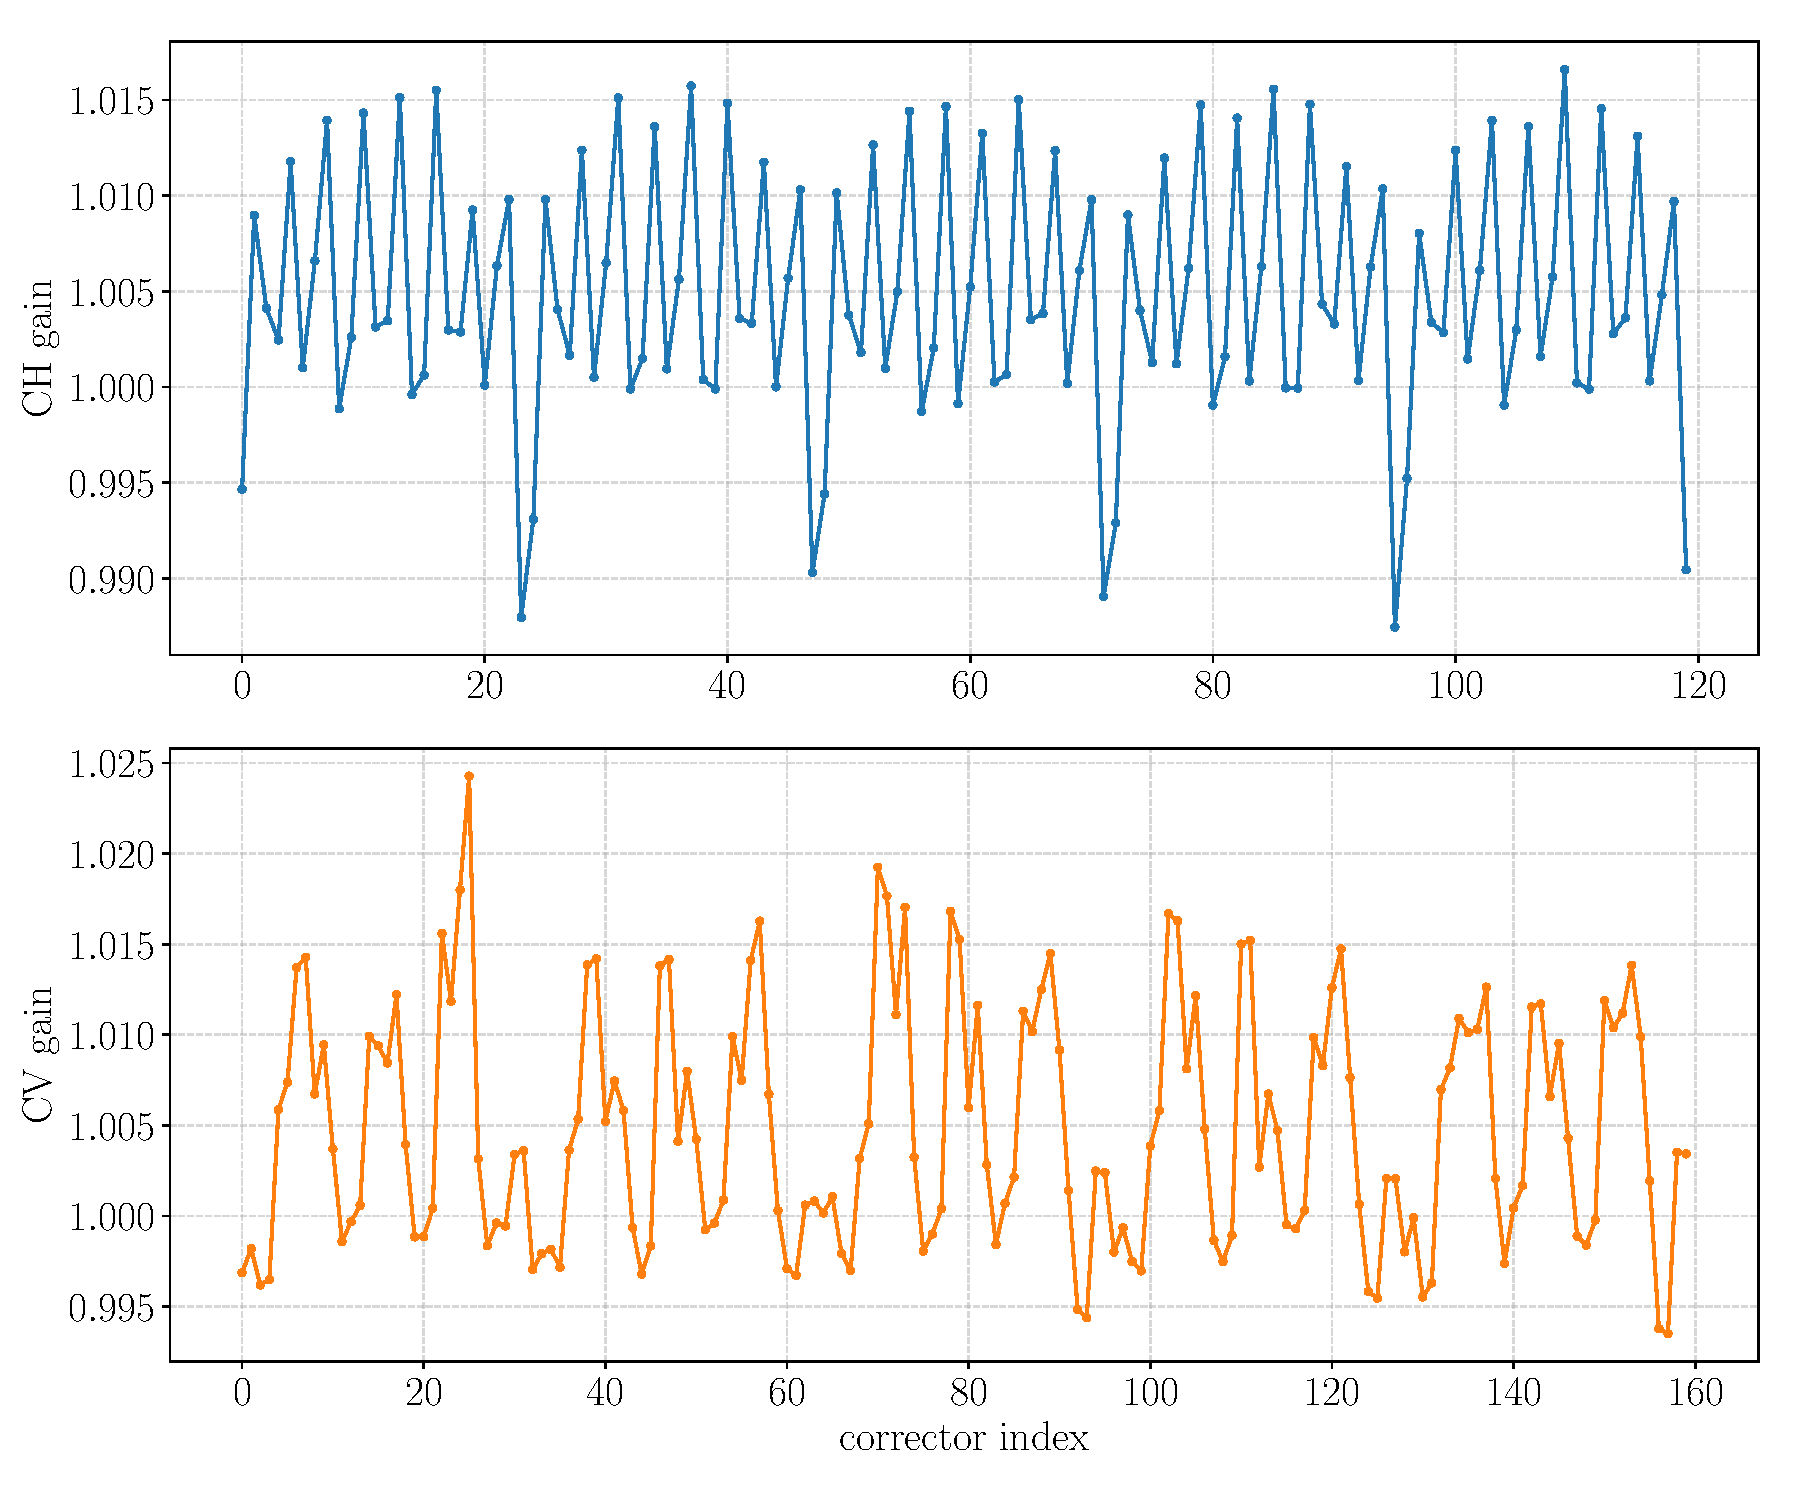
\includegraphics[width=1.0\textwidth]{figures/corr_gains_orbit_distortion.pdf}
    \caption{Correctors gains.}
    \label{subfig:corr_fit_orb}
\end{subfigure}
\caption{Fitted values for BPM gains, roll errors and correctors (CH and CV) gains for model with perturbed orbit.}
\label{fig:gain_fit_orb}
\end{figure}

One can note the periodic signature in the gains. Even though the absolute values are smaller than the gains obtained in the previous fitting (Figure~\ref{fig:gain_fit}), the periodic signature observed previously (especially for correctors) can be related to the ones obtained here. The BPM roll angles adjusted in this test were also on the order of $\pm\SI{10}{\milli\radian}$. Thus the values obtained previously probably are not related to the~\gls{bpm} roll errors and the major contribution might be from the orbit distortion.

The beta-beatings caused by the residual orbit were also calculated and compared with the first LOCO fitting reported in Section~\ref{sec:orm_fit}. The results are presented in Figure~\ref{fig:beta_beating_orb}. The disturbed orbit produced~\gls{std} beta-beatings of $\SI{8.6}{\%}$ in horizontal and $\SI{3.0}{\%}$ in vertical plane. It can be seen that the orbit contributions to the beta-beating in some locations are commensurable to the ones obtained from the calibrated model. The fact that the predicted beta-beating is larger than the one caused by orbit distortion is reasonable, since in the actual storage ring there are other sources of optics perturbations. 
\begin{figure}
\centering
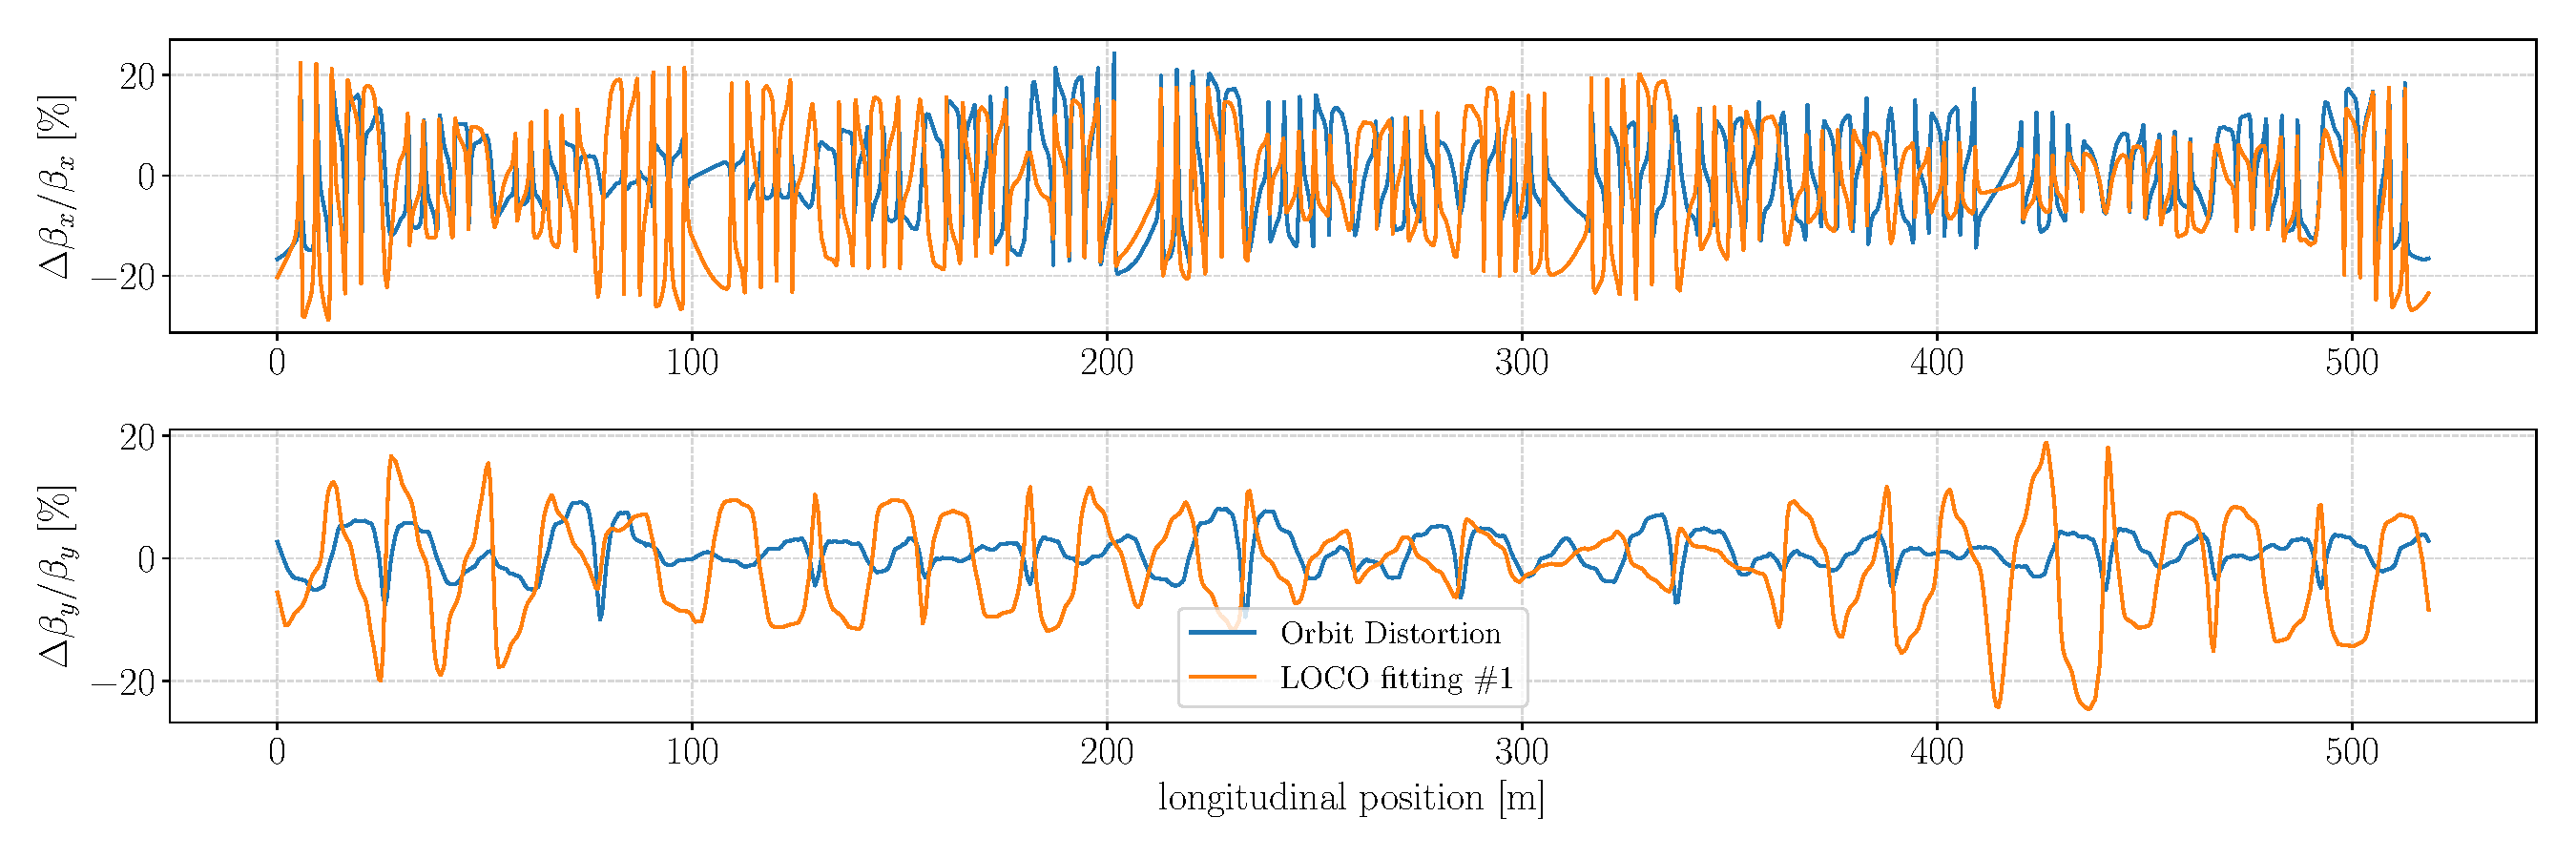
\includegraphics[width=1.0\textwidth]{figures/beta_beating_orbit_loco_iter0.pdf}
\caption{Beta-beating comparison from perturbed orbit model with first LOCO calibrated model.}
\label{fig:beta_beating_orb}
\end{figure}

Another comparison was performed between the dispersion functions from the perturbed orbit model and the measurements realized on storage ring before LOCO corrections, plotted in Figure~\ref{fig:disperson_orb}. Once again, the actual errors are larger than the ones generated by the feed-down effect, as expected. The vertical dispersion signature similarities draw attention. It is clear that the errors in $\eta_y$ caused by orbit distortion explain a substantial part of the measured $\eta_y$. The correlation between measured $\Delta\eta_x$ and the calculated with orbit distortions is $76\%$ and for $\Delta\eta_y$ the correlation is $53\%$. The main sources of $\eta_y$ are vertical bendings created by vertical orbit distortions on quadrupoles.
\begin{figure}
\centering
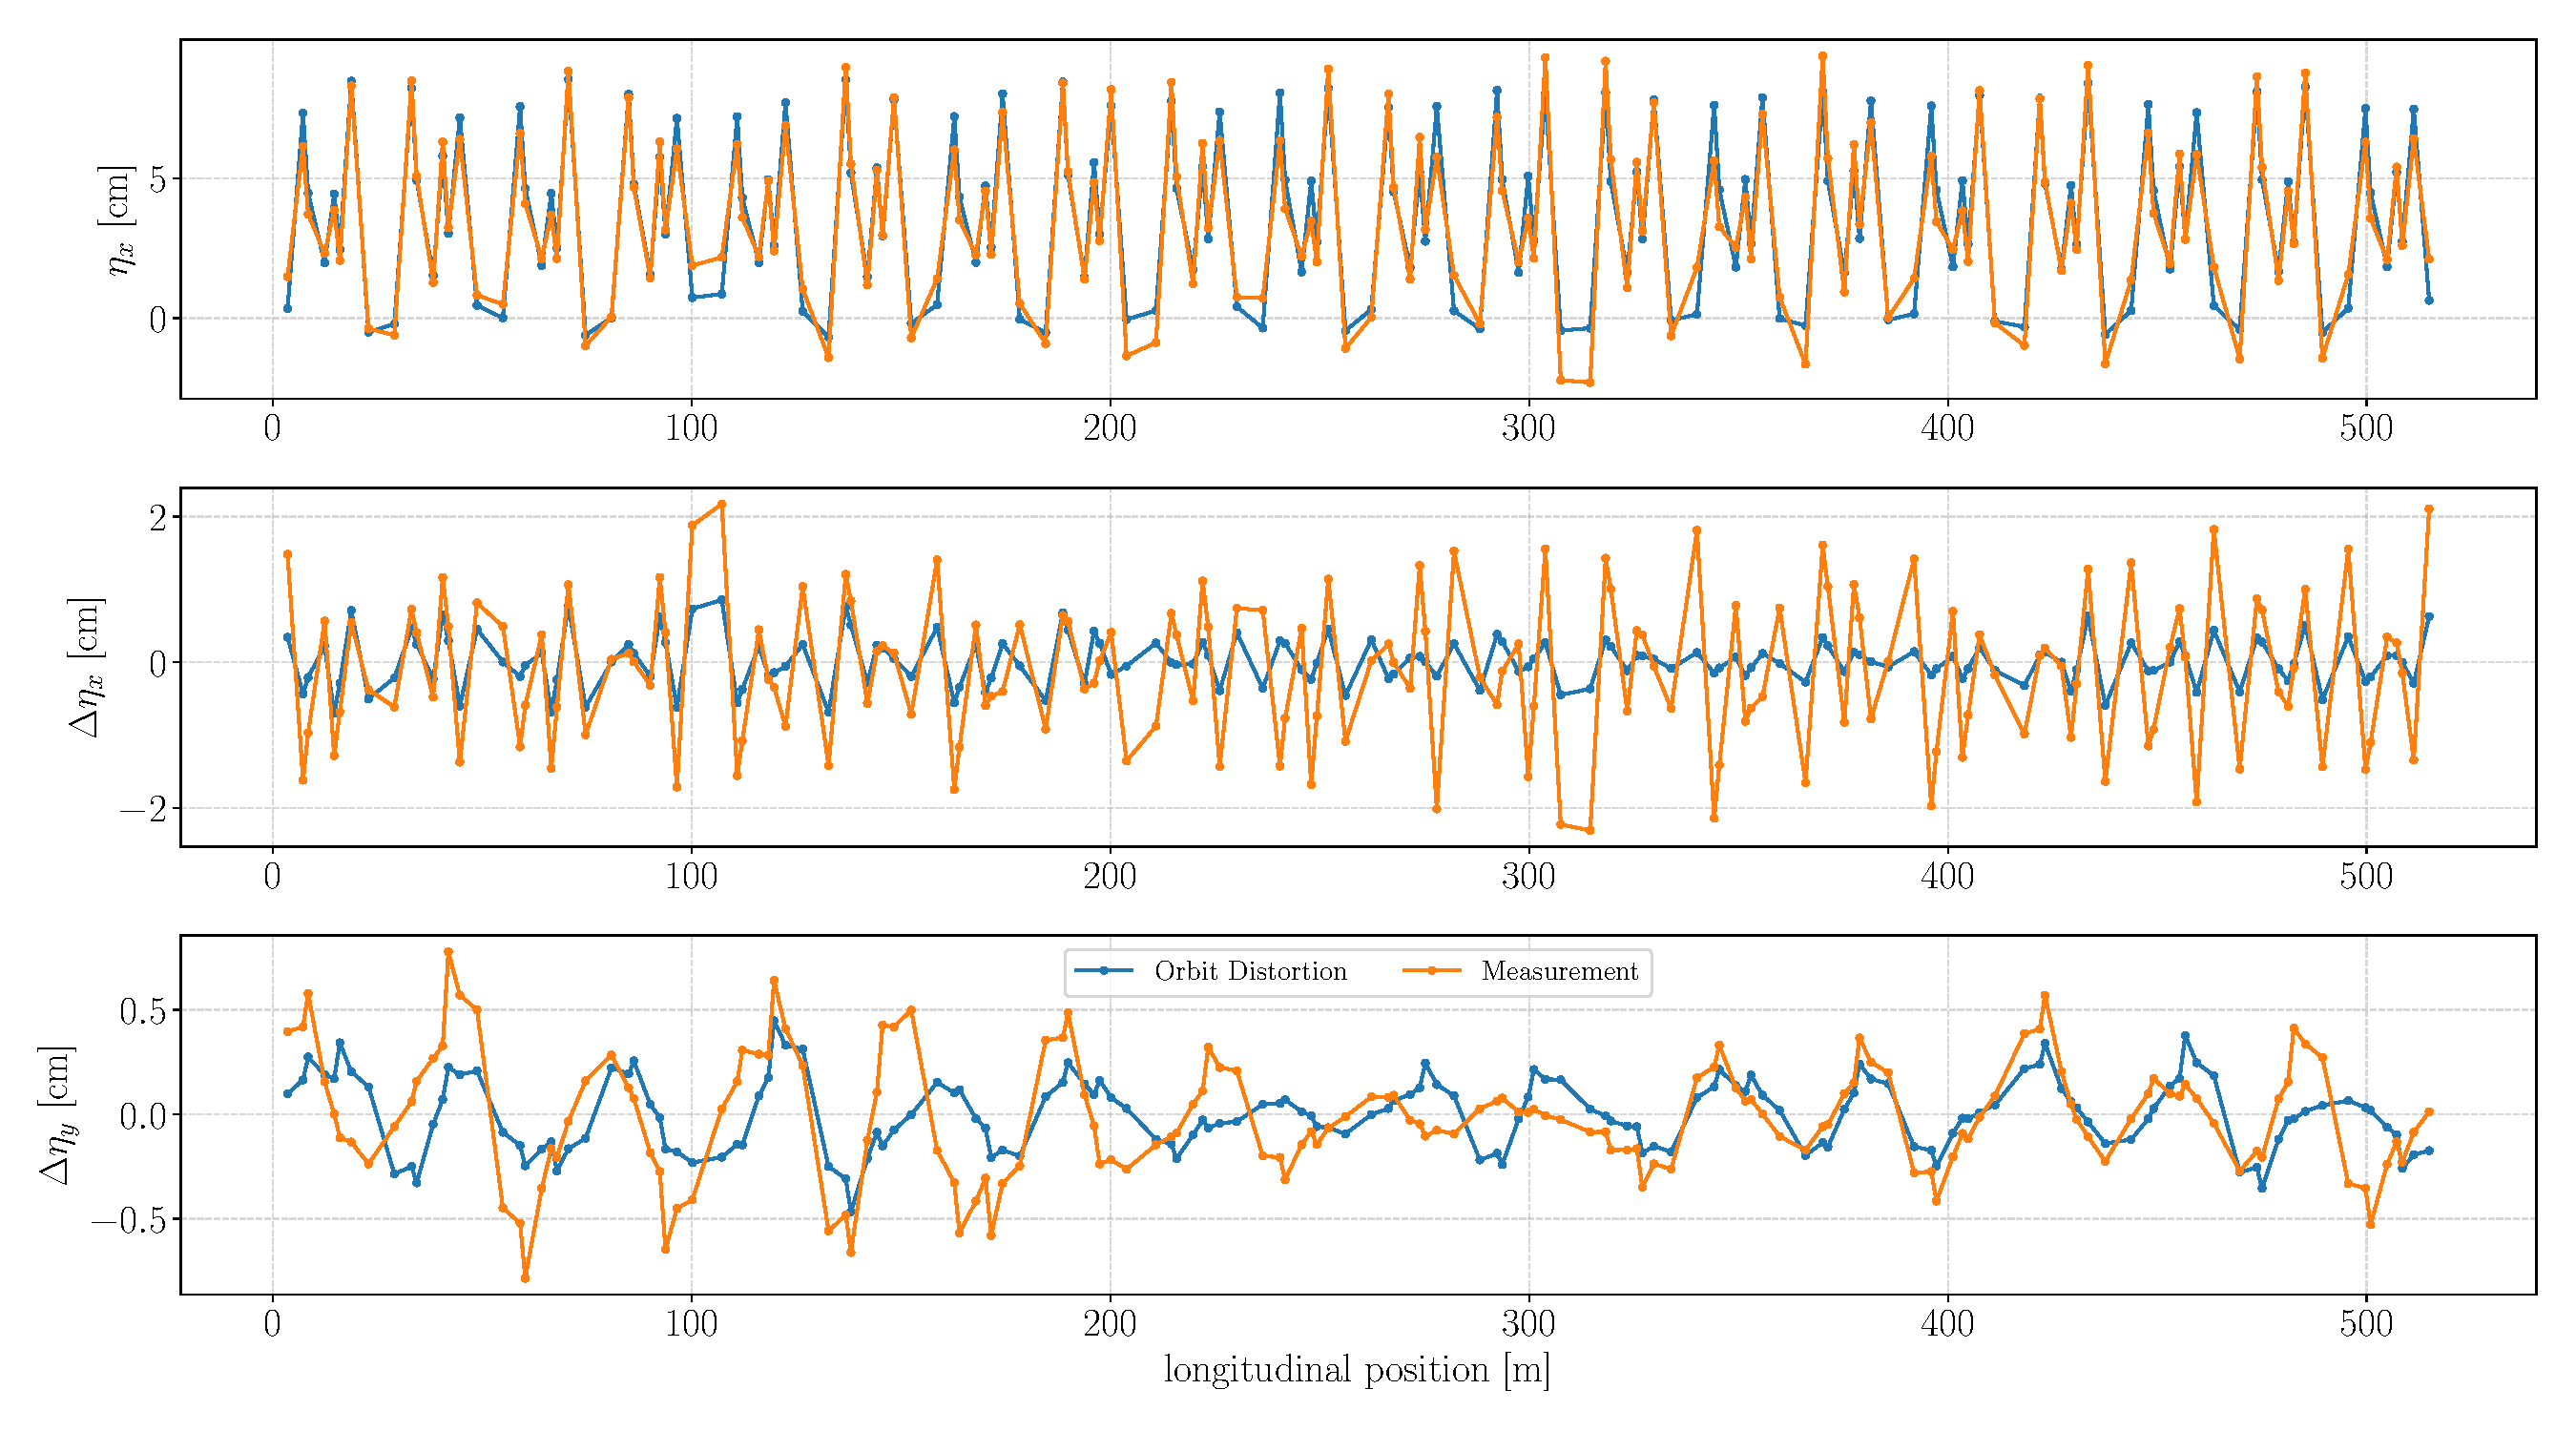
\includegraphics[width=1.0\textwidth]{figures/dispersion_orbit_iter0.pdf}
\caption{Comparison between dispersion functions at BPMs obtained perturbed orbit model with measurement before optics corrections.}
\label{fig:disperson_orb}
\end{figure}

Finally, the variations in normal and skew quadrupoles obtained in this test were compared with LOCO corrections applied in storage ring, as can be seen in Figure~\ref{fig:corrections_orb}.
\begin{figure}
\centering
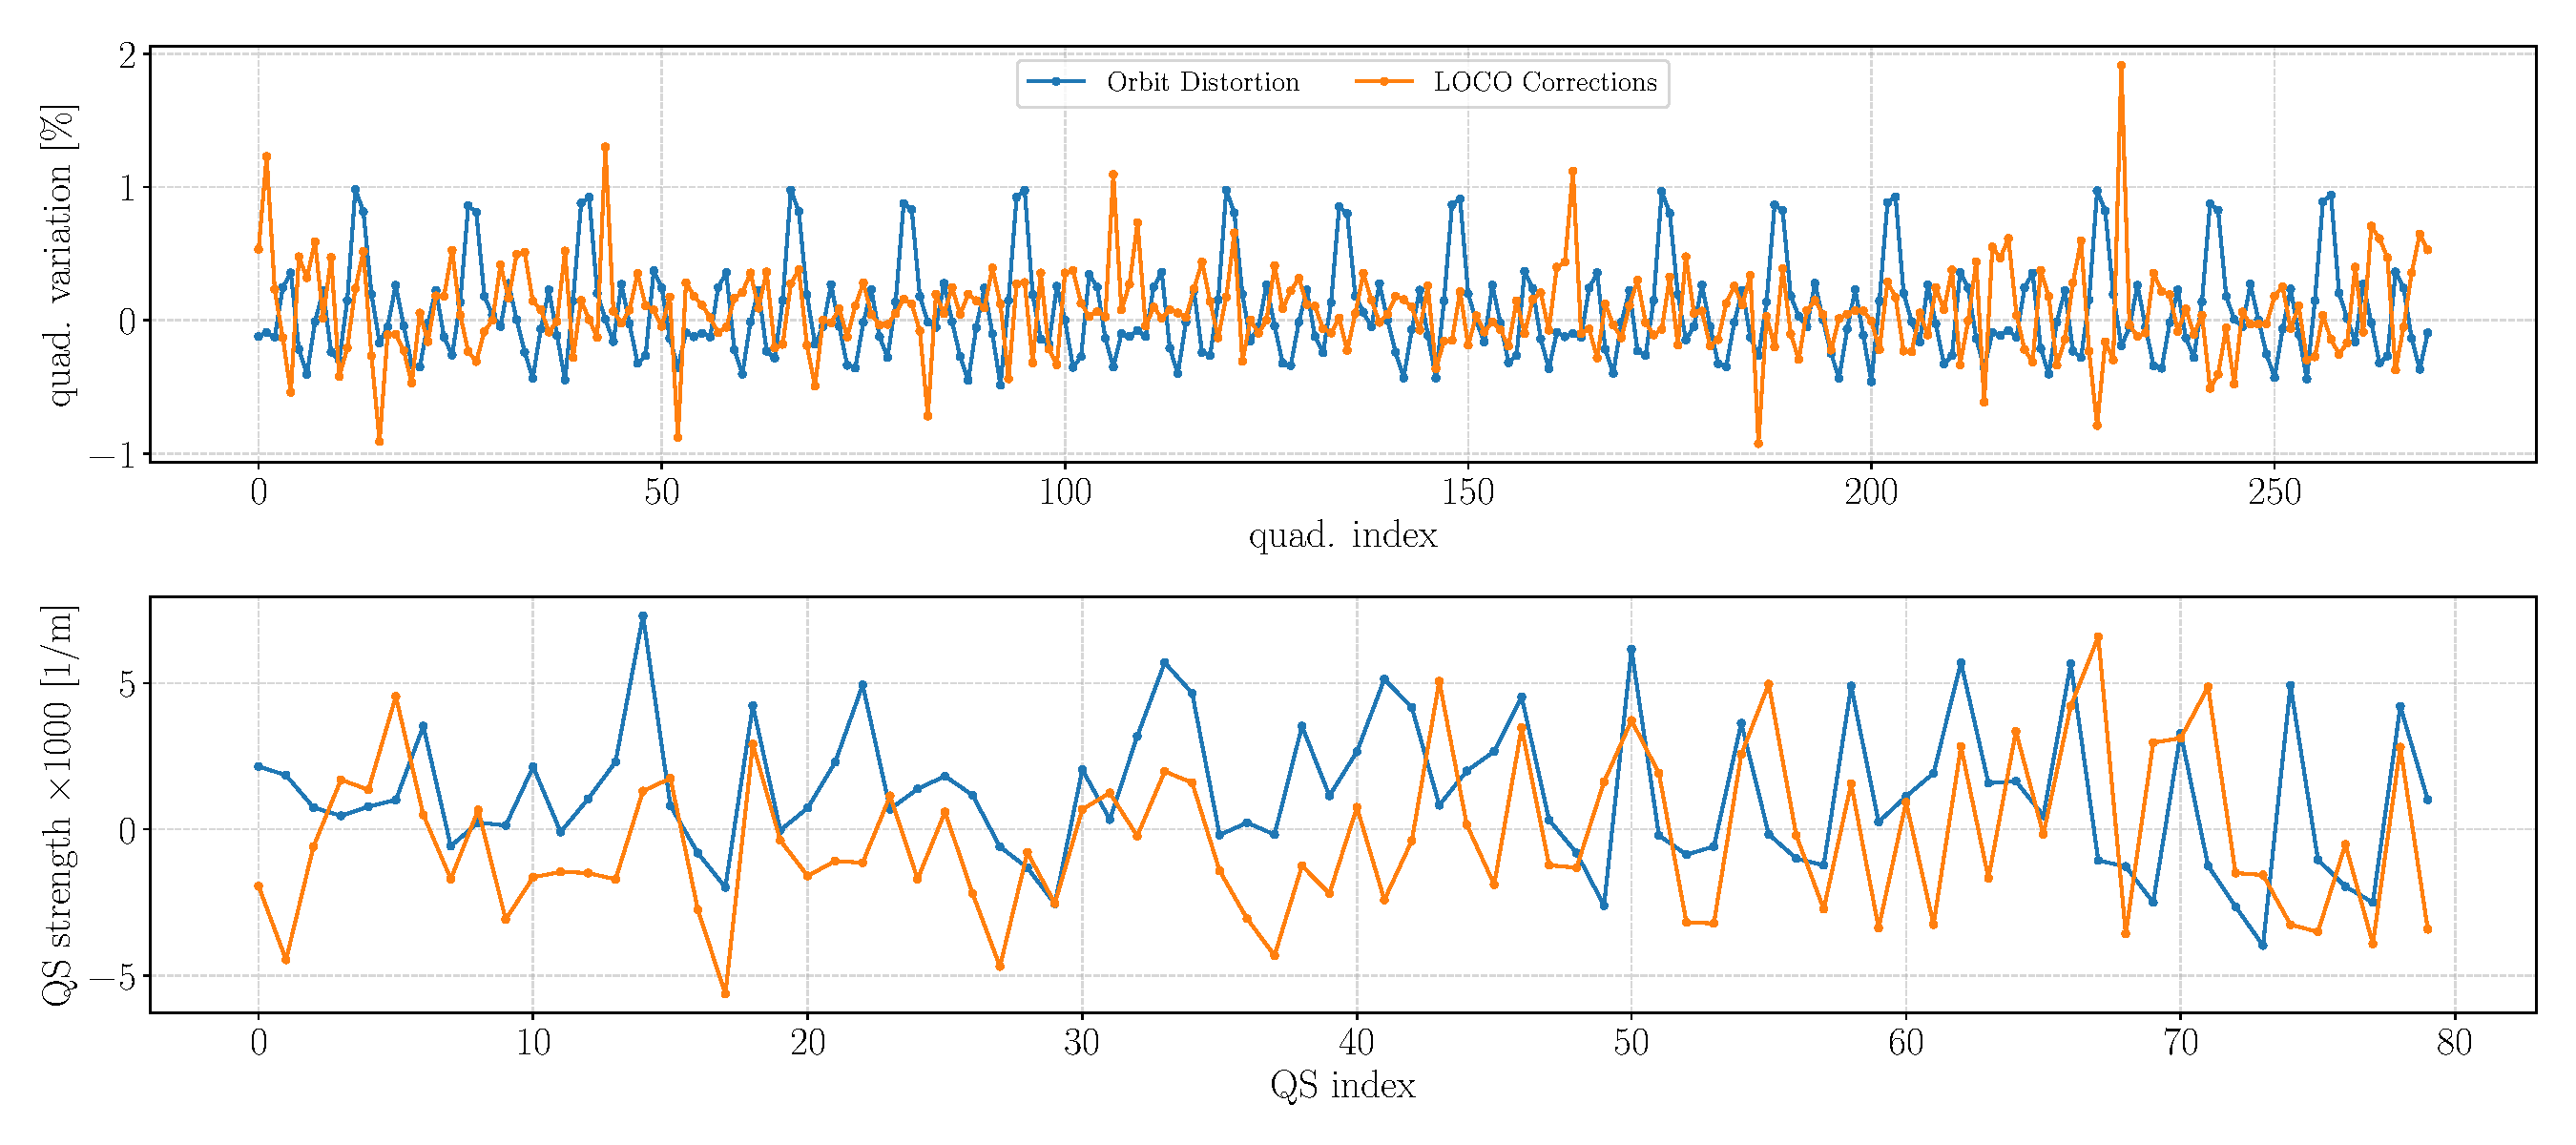
\includegraphics[width=1.0\textwidth]{figures/corrections_orb_residue_loco_iter0.pdf}
\caption{Normal and skew quadrupoles variation for perturbed orbit model and the first LOCO calibrated model.}
\label{fig:corrections_orb}
\end{figure}

The order of magnitude of variations in both cases are very similiar. For quadrupoles, the std variations are $\SI{0.36}{\%}$ for orbit perturbed model and $\SI{0.33}{\%}$ for LOCO corrections. For skew quadrupoles, the std variations are $\SI{2.4e-3}{\meter^{-1}}$ for orbit perturbed model and $\SI{2.7e-3}{\meter^{-1}}$ for LOCO corrections. When these corrections were applied in the perturbed model, the~\gls{orm} errors were greatly reduced, the optics errors are reduced (except for $\eta_y$) but could not be eliminated, exactly as observed in the actual storage ring. The results of optics corrections on perturbed model is organized on Table~\ref{tab:params_corr}.
\begin{table}
    \centering
    \caption{Optics errors before and after LOCO corrections applied on perturbed model.}
    \label{tab:params_corr}
    \begin{tabular}{cccc}
        \toprule\toprule
        Parameter (std) & before corr. & after corr. & Unit\\
        \hline
        $\Delta\beta_x/\beta_x$ & \SI{8.6}{} & \SI{1.8}{} & \SI{}{\%}\\
        $\Delta\beta_y/\beta_y$ & \SI{3.0}{} & \SI{1.5}{} & \SI{}{\%}\\
        $\Delta\eta_x$ & \SI{3.3}{} & \SI{1.6}{} & \SI{}{\milli\meter} \\
        $\Delta\eta_y$ & \SI{1.7}{} & \SI{1.9}{} & \SI{}{\milli\meter}\\    
        \bottomrule\bottomrule
    \end{tabular}
\end{table}

% From this tests its is clear that the orbit plays an important role on Sirius storage ring optics. When the residual orbit measured on the actual ring is reproduced in the model, the behavior of LOCO fitting with measured data was also observed in the fitting of~\gls{orm} generated with the disturbed orbit. More than that, the magnitudes and signatures of betatron and dispersion function disturbances

From these results, it can be seen that, even with nominal gradients on the lattice, the linear optics perturbations generated by orbit distortions could be reduced but there is a limitation for this scheme of correction. The off-diagonal elements in ORM can be greatly reduced with skew quadrupoles, however since the vertical dispersion function could not be adjusted with LOCO fitting, it could not be corrected as well (in fact, the error was even increased). 

The qualitative behavior of LOCO analysis using an ORM calculated from a model with the same residual orbit as measured in Sirius storage ring reproduces the behavior that is observed with measured ORM. Since in the real machine other errors also perturb the linear optics, it is expected that the minimum level of optics correction with a disturbed orbit is higher than the level obtained in this test. 

This test raises a hypotheses for the incapacity of LOCO fitting to predict accurately the storage ring optics. LOCO, as included in the method name, is a process to obtain the linear optics (regarding dipoles and quadrupoles). However, it was verified that the feed-down effects in quadrupoles and sextupoles (due to residual orbits) play an important role in the Sirius optics. An origin for this residual orbit might be the magnets misalignment in the storage ring, which was already confirmed with measurements performed by LNLS Alignment Group. Another explanation for these problems might be the incompatibility between the storage ring model and the actual storage ring regarding the elements longitudinal positions (specially from girders misalignment). In this case, the model would not accurately describe the storage ring.

The betatron function depends basically on the focusing strengths introduced by quadrupoles, while the dispersion function depends both on focusing and deflecting forces. Orbit distortions in quadrupoles introduce additional dipolar fields and in sextupoles extra focusing are introduced by the feed-down effect. With LOCO fitting, only the quadrupoles are varied to fit the linear optics. So, if the quadrupoles are used to compensate the gradients in sextupoles to fix the betatron function, the additional dipolar fields in quadrupole are changed as well, perturbing the dispersion function. On the other hand, if the quadrupoles are used to compensate the dipolar fields in quadrupoles and fix the dispersion function, the focusing strengths along the ring are changed and the betatron functions are perturbed. Therefore, in the presence of large orbit distortions, it is only possible to balance the correction of betatron function without perturbing the dispersion (or vice-versa), reaching a limited level of correction effectiveness.

Furthermore, this type of correction that uses quadrupoles to compensate for perturbations generated by orbit distortion is inadequate. The actual solution is to minimize the alignment problems that limit the residual orbit, so the orbit can be best corrected to the magnetic centers, reducing its effect on linear optics. After that, the LOCO corrections should fix these deviations and the optics errors should be corrected to a better level. A realignment campaign in Sirius is scheduled for January 2021. In this campaign, the devices longitudinal positions will also be measured and will be used to improve the storage ring model. After that, the machine will be re-commissioned and it is expected that LOCO analysis can be performed again to obtain a better level of correction for the storage ring linear optics.
